%File: main.tex
%  HARP paper formatted for AAAI-27 using the official AuthorKit27 style files
%  (aaai2027.sty + aaai2027.bst). Anonymous submission mode.
%
%  Notes on the AAAI-27 style:
%   - aaai2027.sty loads the fonts (newtxtext, helvet, courier), [T1]{fontenc},
%     and the page geometry itself. Do NOT load times/helvet/courier/fontenc or
%     set \pdfpagewidth/\pdfpageheight by hand.
%   - With T1 fontenc active, straight quotes in listings render natively, so the
%     earlier OT1 \textquotedbl problem no longer applies.
%   - Forbidden here and removed from the original ARR source: hyperref, bbm, ulem.
\documentclass[letterpaper]{article} % DO NOT CHANGE THIS
\usepackage[submission]{aaai2027}    % DO NOT CHANGE THIS
% Fonts (newtxtext/helvet/courier) are loaded by aaai2027.sty. DO NOT add
% \usepackage{times}, \usepackage{helvet}, \usepackage{courier}, or fontenc.
\usepackage[hyphens]{url}            % DO NOT CHANGE THIS
\usepackage{graphicx}                % DO NOT CHANGE THIS
\urlstyle{rm}                        % DO NOT CHANGE THIS
\def\UrlFont{\rm}                    % DO NOT CHANGE THIS
\usepackage{natbib}                  % DO NOT CHANGE THIS AND DO NOT ADD ANY OPTIONS TO IT
\usepackage{caption}                 % DO NOT CHANGE THIS AND DO NOT ADD ANY OPTIONS TO IT
\frenchspacing                       % DO NOT CHANGE THIS

% --- Math and formatting packages used by the paper ---
\usepackage{amsmath}
\usepackage{amssymb}
\usepackage{amsfonts}
\usepackage{mathtools}
\usepackage{amsthm}
\usepackage{bm}
\usepackage{algorithm}
\usepackage{algorithmic}
\usepackage{booktabs}
\usepackage{array}
\usepackage{multirow}
\usepackage{enumitem}
\usepackage{subfig}
\usepackage{nicefrac}
\usepackage{microtype}

% --- Listings (used for prompt templates in the appendix) ---
\usepackage{listings}
\usepackage{xcolor}
\definecolor{dkgreen}{rgb}{0,0.6,0}
\definecolor{codegray}{rgb}{0.5,0.5,0.5}
\definecolor{mauve}{rgb}{0.58,0,0.82}

% --- Theorem environments ---
\newtheorem{theorem}{Theorem}[section]
\newtheorem{proposition}[theorem]{Proposition}
\newtheorem{lemma}[theorem]{Lemma}
\newtheorem{corollary}[theorem]{Corollary}
\newtheorem{definition}[theorem]{Definition}
\newtheorem{assumption}[theorem]{Assumption}
\newtheorem{remark}[theorem]{Remark}
\newtheorem{example}[theorem]{Example}

% --- AAAI required metadata ---
\setcounter{secnumdepth}{2}
\pdfinfo{
/TemplateVersion (2027.1)
}

\title{LLM Orchestration under Heterogeneous Preferences\\
via Explicit Persona Inference}

% Anonymous submission: the aaai2027 [submission] option typesets
% "Anonymous submission" and suppresses the author / affiliation block below.
\author{}
\affiliations{}

\begin{document}
% Float placement parameters (LaTeX defaults let floats queue and drift to the
% end of the document; these relax the limits without touching page geometry).
\renewcommand{\topfraction}{0.92}
\renewcommand{\bottomfraction}{0.7}
\renewcommand{\dbltopfraction}{0.92}
\renewcommand{\textfraction}{0.07}
\renewcommand{\floatpagefraction}{0.75}
\renewcommand{\dblfloatpagefraction}{0.75}
\setcounter{topnumber}{3}
\setcounter{dbltopnumber}{3}
\setcounter{bottomnumber}{2}
\setcounter{totalnumber}{5}

\setlength{\textfloatsep}{9pt plus 2pt minus 4pt}
\setlength{\dbltextfloatsep}{5pt plus 2pt minus 2pt}
\setlength{\abovecaptionskip}{3pt}

\maketitle

\begin{abstract}
Coordinating multiple Large Language Model (LLM) agents requires a belief about goals and preferences the coordinator does not observe. Existing LLM-agent methods keep that belief inside the prompt, where it consumes context on every turn and drifts as the model rewrites it. Moving the belief out of the prompt avoids this, but an exact posterior over the joint persona profile is exponential in the number of agents. In this work, we propose \textbf{HARP} (Heterogeneous-preference Agent oRchestration via Personas), a novel framework that tracks personas numerically and plans for all agents centrally. Specifically, HARP keeps one posterior per agent over a discrete persona library and updates each in closed form, so the language model supplies likelihoods rather than storing the belief itself. HARP therefore represents the joint posterior exactly at $O(n|\Theta_i|)$ storage rather than $O(|\Theta_i|^n)$, and incurs the same $\tilde O(\sqrt K)$ Bayesian regret as the explicit joint tracker it replaces. HARP\textsuperscript{+} adds a planning bonus for actions that distinguish personas, which removes the remaining loss from early uncertainty. We evaluate HARP on four substrates spanning a controlled public-goods game, externally authored bargaining payoffs, a ride-hailing dispatch replay, and open-ended dialogue. Across the class our theory identifies, HARP\textsuperscript{+} is the strongest non-oracle method, and it still runs at scales where the explicit joint tracker cannot.
\end{abstract}

\begin{figure*}[t!]
  \centering
  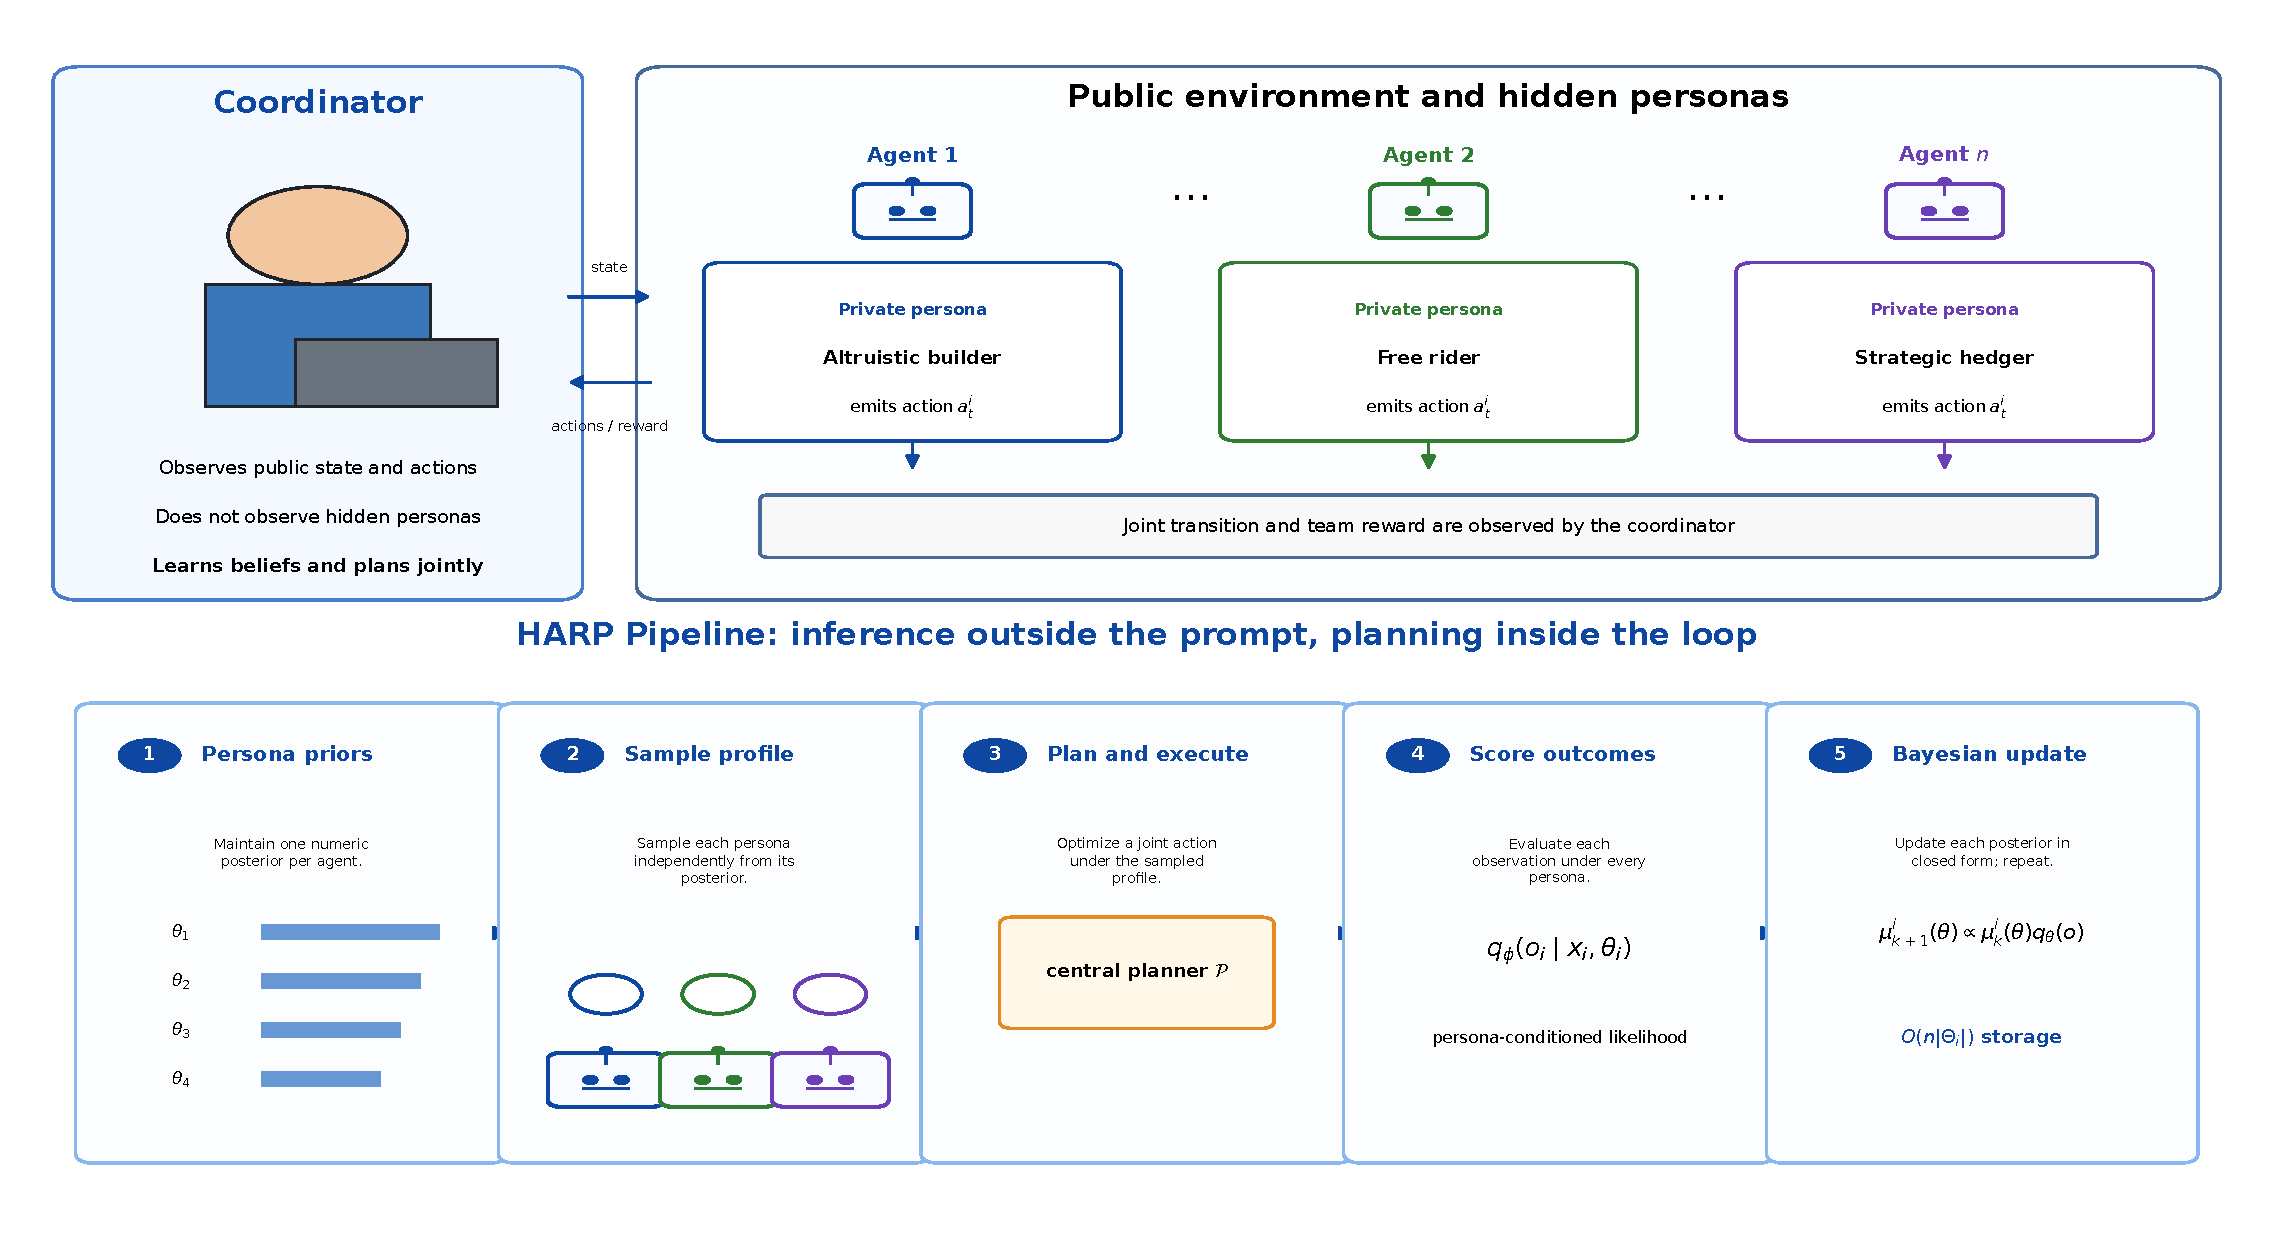
\includegraphics[width=1\textwidth]{figs/main.pdf}
\caption{\textbf{Overview of HARP.} \textbf{Top:} A coordinator interacts with LLM agents in a public environment; each agent has a private persona (e.g., altruistic builder, free rider, strategic hedger) hidden from the coordinator. \textbf{Bottom:} (1) per-agent persona prior; (2) sample a joint profile from per-agent posteriors; (3) plan and execute (HARP\textsuperscript{+} adds a type-discrimination bonus); (4) score each observed outcome under every persona's calibrated outcome scorer; (5) Bayes-update each posterior.}
  \label{fig:main}
\end{figure*}

\section{Introduction}
\label{sec:intro}

Large language models are increasingly deployed as autonomous agents in settings that negotiate, bargain, allocate resources, and provide public goods~\citep{wu2023autogen,li2023camel,hong2024metagpt,park2023generative,meta2022human}. Each agent typically carries a private \emph{persona}, meaning a hidden goal, preference, or constraint that determines how it values outcomes, and these are rarely visible to a coordinator or to the other agents~\citep{zhou2024sotopia,abdulhai2023lmrl}. Consider a ride-hailing platform dispatching orders to independent drivers. A driver may avoid long trips, stay within a familiar zone, or work only under surge pricing, and such preferences surface only through which orders that driver accepts, declines, or reroutes. A coordinator that recovers these preferences routes requests to drivers who will accept them, while one that treats drivers as interchangeable makes avoidable assignment errors~\citep{mu2026adaptive,yi2025debate}. Because the best joint assignment depends on the realized profile rather than on any driver alone, the platform has to maintain and update a belief over each persona as the interaction unfolds.

Existing LLM-agent methods maintain this belief inside the prompt, re-encoding what has been inferred about each agent as natural-language text at every decision step~\citep{yi2025debate,mu2026adaptive}. In-prompt representation is flexible, but the belief has no persistent state, so inference errors propagate across steps and tracking quality depends on the reasoning ability of the backbone~\citep{park2024llm}. Storing the belief numerically outside the prompt removes that failure mode, at an apparent cost in representation size. With $n$ agents each drawing a persona from a library of $|\Theta_i|$ personas, an exact posterior over the joint profile has $|\Theta_i|^n$ entries, and tracking drivers separately does not avoid this, since the best assignment depends on the full profile. The question is therefore whether a numeric belief can be kept small without losing what the joint posterior contributes to the decision.

In this work, we propose \textbf{HARP} (\textbf{H}eterogeneous-preference \textbf{A}gent o\textbf{R}chestration via \textbf{P}ersonas), which represents the belief numerically at a size linear in the number of agents. Specifically, HARP keeps one posterior per agent over a discrete library of persona prompt templates. Each turn it samples a persona profile, plans a joint policy under it, and dispatches the resulting action to each agent. Every agent therefore emits an action token, and the coordinator asks the LLM for the probability of that token under each persona template. These probabilities are the likelihoods in a closed-form Bayes update applied to each posterior independently, so the LLM enters only as a likelihood model over observed actions. The belief is therefore carried forward rather than re-derived at each step, and under three structural conditions the $n$ per-agent posteriors reconstruct the joint one exactly. When those conditions hold only approximately, the reconstruction degrades in proportion to the violation rather than breaking down. The posterior is also a quantity the coordinator can sample from and plan against directly, which is not possible when the belief exists only as a description in the prompt. Because the model is asked only to score actions rather than to remember what it has inferred, tracking quality no longer depends on its ability to maintain a belief in text.

Our contributions can be summarized as follows. Firstly, we introduce HARP, a novel framework that replaces in-prompt belief reasoning with a closed-form Bayesian update and plans centrally in the joint action space. HARP\textsuperscript{+} adds a planning bonus for actions that distinguish personas, which bounds the early loss by a constant even when the personas are hardest to separate. Secondly, we state three structural conditions under which the per-agent posteriors reconstruct the joint one exactly, so storage and update work drop from $O(|\Theta_i|^n)$ to $O(n|\Theta_i|)$. The Bayesian regret is unchanged, since HARP reproduces the explicit joint tracker pathwise under matched seeds. Finally, we evaluate HARP on four substrates spanning a controlled public-goods game, a bargaining benchmark with externally fixed payoffs, a ride-hailing dispatch replay, and open-ended dialogue. Under a control that fixes the persona profile, prior, payoffs, and exact optimum across methods, HARP\textsuperscript{+} attains the lowest regret of any non-oracle method on all four backbones. Its cumulative regret remains bounded on both the public-goods and bargaining substrates, whereas sampling personas without updating them incurs regret that grows linearly in the number of episodes. Permuting the posteriors across agents returns regret to the level of not updating at all, which locates the advantage in the identity of the inferred personas rather than in the presence of a belief. On the dispatch substrate the margin over the strongest in-prompt baseline widens as competition for the same orders increases, and it is obtained at agent counts for which an explicit joint table is infeasible.

\section{Related Work}
\label{sec:related}

\paragraph{Bayesian and latent-type reinforcement learning.} Posterior sampling attains near-optimal Bayesian regret for a single agent by drawing one model from the posterior each episode and planning as if it were correct~\citep{strens2000bayesian,osband2013more,agrawal2017optimistic,ouyang2017learning,russo2014learning,russo2016information,dasgupta2025bayesian}. Extensions to Markov games largely assume known types or zero-sum structure~\citep{jahromi2024bayesian,xiong2022self}, and learning in latent Markov decision processes is exponentially hard without an identifiability condition~\citep{kwon2021rl,nguyen2024learning}, which is the role our structural conditions play. Type-based ad hoc teamwork already keeps a separate belief per teammate~\citep{albrecht2015game,albrecht2019convergence,barrett2011empirical,albrecht2018autonomous}, so our contribution is not that representation but the conditions under which it is exact and the finite-time regret it attains at linear storage. Structured Bayesian priors~\citep{mutti2024exploiting} and language-model posterior sampling~\citep{arumugam2025toward} do not factor the belief across agents, while general-sum Markov-game learning~\citep{jin2024v,song2021can,mao2023provably,erez2023regret,yang2025incentivize} and population-based training~\citep{lanctot2017unified,muller2019generalized,marris2021multi} address equilibrium selection rather than inference over partner types.

\paragraph{Structural decomposition.} Avoiding a joint object by exploiting structure is long established. Networked distributed POMDPs decompose the value function along an interaction graph~\citep{nair2005networked,oliehoek2008exploiting}, restless-bandit formulations decouple joint allocation into per-arm indices by Lagrangian relaxation~\citep{mate2020collapsing}, and Bayesian Stackelberg solvers avoid expanding the game over the joint type space of an unknown follower~\citep{paruchuri2008playing}. We instead factor the posterior over partner personas, the factorization introduces no approximation, and the personas are inferred online rather than supplied as a fixed prior.

\paragraph{Language-model agents and coordination.} Recent language-model agents reason explicitly about their partners but differ in what the belief is made of. ECON learns a belief representation over co-agent strategies and drives the group toward a Bayesian Nash equilibrium~\citep{yi2025debate}, Hypothetical Minds keeps a natural-language hypothesis per partner and rewrites it when it fails~\citep{cross2025hypothetical,li2023theory}, and A-ToM selects among reasoners of different theory-of-mind order by expert advice~\citep{mu2026adaptive,cesa1997use}. All are interactive-POMDP formulations~\citep{gmytrasiewicz2005framework} whose belief is generated as text or learned end to end, so the coordinator cannot condition on it directly. Orchestration frameworks~\citep{wu2023autogen,li2023camel,hong2024metagpt,park2023generative,chen2023autoagents} and negotiation systems~\citep{meta2022human,abdulhai2023lmrl} treat partner modeling as a by-product of role prompting or a learned reward~\citep{agashe2025llm}. HARP keeps an explicit posterior over a fixed persona library and updates it in closed form, without training a belief model of its own.

\section{Methodology}
\label{sec:algorithm}

\subsection{Preliminaries and Definitions}
\label{sec:setting-main}

We formulate LLM multi-agent coordination as a Bayesian inference problem. A coordinator interacts with $n$ LLM agents over $K$ episodes of $H$ turns. Each agent $i$ carries a private persona $\theta_i^\star \in \Theta_i$ supplied through its system prompt, and the joint profile $\boldsymbol\theta^\star \in \boldsymbol\Theta = \prod_i \Theta_i$ is drawn once from a prior $P_0^\Theta$ and then held fixed. The environment evolves under an unknown transition kernel $P^\star$, and each agent receives a reward $r_i(s,a,\theta_i^\star)\in[0,1]$ that depends on its own persona. Neither $\boldsymbol\theta^\star$ nor $P^\star$ is revealed, so both are inferred from the trajectories the interaction produces.

At each turn the coordinator plans from its current posterior and the public state, using a fixed deterministic map $\mathcal P$ that takes a sampled world $(P,\boldsymbol\theta)$ to a joint policy. Every agent then acts, and the coordinator records the actions taken, the rewards received, and the next state. Performance is measured by cumulative Bayesian regret against the policy the same map $\mathcal P$ returns under full knowledge of $(P^\star,\boldsymbol\theta^\star)$, so the comparison isolates what is lost to uncertainty about the world rather than to the quality of the planner. In the finite substrates we evaluate, $\mathcal P$ is an exhaustive joint-action argmax with deterministic tie-breaking, while the open-ended dialogue substrate generates text directly and admits no finite planner. Full notation and formal definitions are in Appendix~\ref{sec:setting-app}.

\subsection{HARP}
\label{sec:pact-vanilla}

HARP keeps one numeric posterior $\mu_k^{\Theta,i}$ per agent over the persona library, together with a model posterior $\mu_k^P$, and couples both to the centralized planner $\mathcal P$ (Algorithm~\ref{alg:pact}). Each episode it samples a world $(\hat P_k, \hat{\boldsymbol\theta}_k)$ from these posteriors and calls $\mathcal P$ for a joint policy. After the episode, each agent's belief updates independently as
\begin{equation}
\label{eq:likelihood}
\resizebox{0.90\linewidth}{!}{$\displaystyle
\mu_{k+1}^{\Theta,i}(\theta_i) \;\propto\; \mu_k^{\Theta,i}(\theta_i)\prod_{h=1}^{H} q_\phi(o_{i,h}^k\mid x_{i,h}^k,\theta_i)
$}
\end{equation}
where $x_{i,h}^k$ is the public context and $o_{i,h}^k$ the observed action and reward. The likelihood $q_\phi$ scores what was observed against what each persona in the library would predict, so the update requires no gradient step and no belief model of its own.

\begin{algorithm}[t]
\caption{HARP (and HARP\textsuperscript{+} with $\beta>0$)}\label{alg:pact}
\textbf{Input}: priors $P_0^P, \{P_0^{\Theta,i}\}$; horizon $H$; episodes $K$; deterministic centralized planner $\mathcal P$; bonus coefficient $\beta\geq 0$.\\
\begin{algorithmic}[1]
\STATE Initialize $\mu_1^P\!\gets\! P_0^P$, $\mu_1^{\Theta,i}\!\gets\! P_0^{\Theta,i}$ for all $i$.
\FOR{$k=1,\dots,K$}
  \STATE Sample $\hat P_k\!\sim\!\mu_k^P$ and $\hat\theta_i^k\!\sim\!\mu_k^{\Theta,i}$ independently.
  \STATE If $\beta>0$: compute $D_k(s,a)$ via Eq.~\eqref{eq:bonus} and add $\beta D_k$ to $Q$ in backward induction.
  \STATE $\pi_k\gets\mathcal P(\hat P_k,\hat{\boldsymbol\theta}_k)$; execute $\pi_k$, observe $\tau_k$.
  \STATE Bayes-update each marginal independently from $\tau_k$.
\ENDFOR
\end{algorithmic}
\end{algorithm}

The factored belief stores $O(n|\Theta_i|)$ entries, whereas the naive joint posterior $\mu_k(\boldsymbol\theta^\star)$ has $|\boldsymbol\Theta| = \prod_i |\Theta_i|$, exponential in $n$. The two agree exactly only on a restricted class of coordination problems, which we now describe. Three structural conditions are jointly sufficient, and (TI) and (RL) are each necessary for the likelihood to split across agents (Appendix~\ref{app:necessity}).

\begin{assumption}[Structural conditions]
\label{ass:struct}
\textbf{(TI) Transition independence.} Environment dynamics do not depend on the persona profile: $P^\star(s' \mid s, a, \boldsymbol\theta) = P^\star(s' \mid s, a)$.
\textbf{(RL) Reward locality.} Each agent's reward depends only on its own persona: $r_i(s, a, \boldsymbol\theta) = r_i(s, a, \theta_i)$.
\textbf{(PF) Prior factorization.} The coordinator's prior over personas factors across agents: $P_0(\boldsymbol\theta^\star) = \prod_i P_0^{\Theta,i}(\theta_i^\star)$.
\end{assumption}

Each condition is checkable on a given problem rather than assumed of social interaction in general. (TI) holds when the transition rule is persona-blind. (RL) holds when an agent's payoff does not depend on the personas of others, and so excludes cross-agent utilities such as envy or spite, $r_1 = r_1^{\theta_1} - \alpha r_2^{\theta_2}$, which break the factored update (Appendix~\ref{sec:necessity}). (PF) holds when slots are filled independently from a persona library. Together they define the class on which posterior decoupling is exact, and bounded violations degrade it gracefully (Appendix~\ref{app:approx-decoupling}).

\begin{theorem}[Posterior Decoupling]
\label{thm:decoupling-main}
Under Assumption~\ref{ass:struct}, the joint posterior over $(P^\star, \boldsymbol\theta^\star)$ at every episode $k$ factors exactly into
\[
P(P, \boldsymbol\theta \mid \mathcal{H}_k) \;=\; \mu_k^P(P) \cdot \prod_{i=1}^n \mu_k^{\Theta,i}(\theta_i),
\]
where each persona marginal $\mu_k^{\Theta,i}$ follows the per-agent Bayes update in Eq.~\eqref{eq:likelihood}. Posterior storage is $O(n|\Theta_i|)$ rather than $O(|\Theta_i|^n)$.
\end{theorem}

The proof factors the trajectory likelihood across agents using (TI) and (RL) and closes by induction on $k$ under (PF). The full argument is in Appendix~\ref{app:decoupling-proof}. The cost of representing and updating the persona belief is therefore linear in the number of agents.

\paragraph{Complexity.} Per episode, HARP performs one planner call over the joint action menu and $nH|\Theta_i|$ closed-form likelihood evaluations, and it stores $O(n|\Theta_i|)$ persona parameters beside the model posterior. In the finite substrates the planner is backward induction with exhaustive joint-action argmax, reducing to one-step enumeration where the horizon is one. Where the outcome scorer is calibrated offline the likelihood reduces to a Gaussian reward factor with an uninformative action factor, so the tracker issues no model queries online. Appendix~\ref{app:cost-accounting} reports measured call and token costs.

\subsection{HARP\textsuperscript{+}: Type-Discrimination Bonus}
\label{sec:pact-plus-algo}

A coordinator that plans only for reward has no reason to prefer actions that reveal who it is coordinating with. When the reward-maximizing action also separates the personas in the library, HARP identifies them at no extra cost. When it does not, the same action is optimal under every persona, the observations carry no information about type, and the posterior stays near the prior however many episodes pass. Appendix~\ref{app:pact-plus} makes this worst case precise as the \emph{deep-trap} family. HARP\textsuperscript{+} supplies the missing incentive with a small planning bonus at each $(s,a)$ where personas differ under the planner's outcome scorer,
\begin{equation}
\label{eq:bonus}
D_k(s,a) \;\coloneqq\; \sum_{i=1}^n \mathbb{E}_{\theta, \theta' \sim \mu_k^{\Theta,i}}\!\big[|r_i(s,a,\theta) - r_i(s,a,\theta')|\big],
\end{equation}
where $\theta$ and $\theta'$ are drawn independently from $\mu_k^{\Theta,i}$, recomputed once per episode, and held fixed within its backward induction. The coefficient $\beta=0.25$ is selected once and then frozen across every substrate and backbone. The bonus costs $O(n|\Theta_i|^2)$ per state-action pair inside the same backward-induction pass (Algorithm~\ref{alg:pact}, line 4), biases planning toward type-revealing actions, and vanishes as the posterior concentrates. Setting $\beta=0$ recovers HARP.

\paragraph{Theoretical guarantees.}

The factored posterior compresses the belief, and the discrimination bonus gives the planner a reason to sharpen it. Under the three structural conditions neither is paid for asymptotically, since the compression is exact and the resulting regret matches that of an explicit joint tracker at storage linear in the number of agents. Theorem~\ref{thm:decoupling-main} establishes the first half, and the theorem below establishes the second.

\begin{theorem}[Per-agent Bayesian regret of HARP]
\label{thm:regret-main}
Let initial states be drawn independently of the model and of the sampling randomness, let the coordinator use an $\epsilon_{\mathrm{plan}}$-approximation of a fixed measurable deterministic planner $\mathcal P$, and place a Dirichlet prior on $P^\star$. Under Assumption~\ref{ass:struct}, for every agent $i$,
\begin{equation}\label{eq:regret-main}\resizebox{0.9\linewidth}{!}{$\displaystyle
\mathbb E\big[\mathrm{Reg}_i^B(K)\big] \;\le\; \tilde O\big(H^{3/2}\sqrt{S A_{\mathrm{joint}} K}\big) + O\big(H\sqrt{|\Theta_i|\,\mathcal H(P_0^{\Theta,i})\,K}\big) + K\epsilon_{\mathrm{plan}}, $}
\end{equation}
where $A_{\mathrm{joint}}=\prod_i|\mathcal A_i|$ and $\mathcal H(P_0^{\Theta,i})$ is the entropy of agent $i$'s persona prior. The full statement and proof are in Appendix~\ref{app:theory}.
\end{theorem}

Where the planner enumerates its action menu exactly, $\epsilon_{\mathrm{plan}}=0$, which covers every finite substrate we evaluate. The bound is not claimed for the open-ended dialogue substrate, which admits no finite planner. The rate matches single-agent posterior sampling while storing $O(n|\Theta_i|)$ persona parameters. The persona term depends only on the per-agent library and prior entropy, never on the joint space $\prod_j|\Theta_j|$, so prior knowledge about one agent reduces regret directly, while a confidently wrong prior inflates a $K$-independent constant instead of changing the rate. When personas are separated by a margin $\rho$ in the observation channel, that term collapses to a constant. On the deep-trap family, HARP\textsuperscript{+} bounds the early loss by a constant for any $\beta>0$. Under matched seeds HARP is pathwise identical to the explicit joint tracker, and removing reward locality alone forces the exponential rate back. Appendix~\ref{app:theory} collects these results, together with the extension to misspecified scorers and a preregistered study that measures the predicted contraction at slope one.

\section{Numerical Evaluation}
\label{sec:experiments-llm}

The guarantees above hold wherever the three structural conditions do, but they do not settle whether the predicted advantage survives contact with language models that generate their own actions. We therefore evaluate HARP on four substrates and four backbones under a control that equalizes everything except how the belief is maintained, and find that a numeric posterior coordinates better than in-prompt tracking while remaining affordable at scales where explicit joint inference cannot run. Three questions organize the evaluation.
\begin{itemize}[leftmargin=1.5em, itemsep=0.2em, topsep=0.2em, parsep=0pt]
\item \textbf{RQ1 (representation):} Does a numeric out-of-prompt posterior improve coordination over in-prompt textual belief maintenance?
\item \textbf{RQ2 (computation):} Does the factored posterior match explicit joint inference in regret while cutting persona storage and update work to $O(n|\Theta_i|)$?
\item \textbf{RQ3 (attribution):} How do the closed-form update, identity attachment, the discrimination bonus, and centralized dispatch each contribute to the gains?
\end{itemize}



The substrates form successive layers of evidence. HP-SPGG (Section~\ref{sec:hp-spgg}) imposes the three conditions by construction, so it is where the size of the gain is measured (RQ1), where the factored and joint posteriors are compared on the same realizations (RQ2), and where each component is removed in isolation under a matched control (RQ3). Concordia (Section~\ref{sec:concordia}) contributes externally fixed payoffs and tests whether the gain survives them (RQ1), whether the factorization holds across configurations (RQ2), and when each component matters (RQ3). MaaSSim (Section~\ref{sec:maassim}) replays a ride-hailing dispatcher and tests how the margin grows as personas become decision-relevant (RQ1), whether inference stays feasible at the agent counts involved (RQ2), and whether the gain traces to correct identity attachment (RQ3). Open-ended dialogue, where the conditions can be neither imposed nor checked, is reported separately in Appendix~\ref{app:sotopia-detail}. The benchmarks use four LLM backbones (DeepSeek-V3.2, GPT-5.4-nano, Kimi-K2.6, Llama-4-Maverick-17B-128E-Instruct-FP8), the case study a single pinned backbone.




\subsection{HP-SPGG: Controlled Diagnostic Benchmark}
\label{sec:hp-spgg}


\paragraph{Setup.} In HP-SPGG (heterogeneous-persona public-goods game), a coordinator oversees $n{=}3$ player LLMs over $K{=}20$ episodes. Each player's hidden type is drawn once, uniformly and independently, from $|\Theta_i|{=}4$ persona archetypes spanning the taxonomy of \citet{fischbacher2001people}, so (TI), (RL), and (PF) all hold by construction. The outcome scorer is calibrated once offline from the same backbone, which makes the likelihood a Gaussian reward factor with $\sigma{=}0.08$. The full specification is in Appendix~\ref{app:llm-supplements}, and the PF prior and DGP probes are in Appendix~\ref{app:structural-boundary}.

\begin{figure}[t]
  \centering
  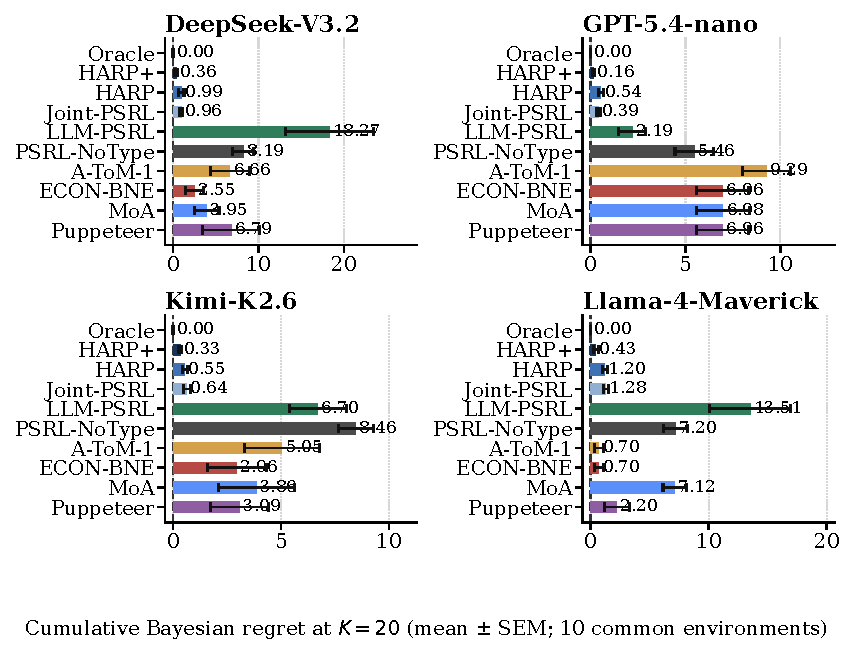
\includegraphics[width=\columnwidth]{figs/fig_e_a_hp_spgg_matched.pdf}
  \caption{Cumulative Bayesian regret on HP-SPGG at $K{=}20$ for four LLM backbones. Within each backbone every method is given the same type profiles, the same uniform prior, the same payoff tensor, and the same exact oracle, and each draws its own realized rewards from that tensor. Values are means over $10$ common seeds and error bars are the standard error of the mean.}
  \label{fig:hp-spgg-cross-model}
\end{figure}


\paragraph{Baselines.} Baselines are Oracle, HARP\textsuperscript{+}, HARP, Joint-PSRL, LLM-PSRL, PSRL-NoType, A-ToM-1, and ECON-BNE, defined in Appendix~\ref{app:llm-supplements}.

\paragraph{RQ1: numeric versus in-prompt beliefs.} To isolate the effect of where the belief is kept, every method within a backbone is given the same hidden type profile, the same uniform prior, the same payoff tensor, and the same exact optimum, so the only difference between them is how the persona belief is represented and updated. We run ten common seeds per backbone and report cumulative Bayesian regret at $K{=}20$. As Figure~\ref{fig:hp-spgg-cross-model} shows, HARP\textsuperscript{+} attains the lowest non-oracle mean regret on every backbone, at $0.360\pm0.142$ on DeepSeek, $0.159\pm0.038$ on GPT-5.4-nano, $0.325\pm0.088$ on Kimi, and $0.430\pm0.217$ on Llama. The strongest comparator that keeps its belief inside the prompt incurs between $1.63$ and $43.77$ times that regret, and LLM-PSRL between $13.8$ and $50.8$ times. Moving the belief out of the prompt therefore improves coordination under a control that holds everything else fixed.

\begin{figure}[t]
  \centering
  
\includegraphics[width=\columnwidth]{figs/fig_e3_n_agent_scaling_v3.pdf}\\[1pt]
  
\includegraphics[width=\columnwidth]{figs/fig_e_g_ladder_v1.pdf}
  \caption{\emph{Top}: cumulative regret on HP-SPGG by agent count (Llama-4-Maverick, $|\Theta_i|{=}4$, $K{=}20$). The aligned storage strip compares factored and joint persona states on a log scale and annotates their ratio; the shaded column marks $n{=}2$, where the joint table is still small. \emph{Bottom}: cumulative regret for HARP\textsuperscript{+} with one belief component removed, and for decentralized execution, on a log scale with the oracle at zero. Values are means over $10$ common seeds and whiskers are the standard error of the mean.}
  \label{fig:storage-vs-regret}\label{fig:component-ladder}
\end{figure}

\paragraph{RQ2: factored versus explicit joint inference.} To test whether the factored posterior gives anything up, we run it and an explicit joint tracker on the same realizations under the same control, so that any difference between them is attributable to the representation alone. The two agree within seed-level standard error on every backbone, differing by $0.030$, $0.153$, $0.095$, and $0.074$ in absolute regret, while the factored representation uses $5.3\times$ fewer persona parameters at $n{=}3$ and $51\times$ fewer at $n{=}5$ (Figure~\ref{fig:storage-vs-regret}). This is the finite-sample counterpart of Theorem~\ref{thm:decoupling-main}. Repeating the comparison analytically, where the two can be run to larger populations, they remain identical to $n{=}8$, past the point at which the joint tracker exhausts memory (Appendix~\ref{app:scaling}). We also test outside the class by drawing personas from a coupled data-generating process that violates prior factorization, where HARP stays within $1.52\times$ of the correctly supported joint baseline (Appendix~\ref{app:structural-boundary}). The compression is therefore free inside the class and degrades gracefully outside it.

\begin{figure*}[t!]
  \centering
  
\includegraphics[width=0.78\textwidth]{figs/fig_maassim_combined_v21.pdf}
  \caption{MaaSSim dispatch. \emph{(a)} Realized utility across conflict strength $\lambda\in\{0,0.5,1\}$ at reject penalty $5$. \emph{(b)} Oracle regret in reject-penalty units, a scale that tracks excess driver rejects, with residual deviations reflecting lost served rides. \emph{(c)} Realized utility for each source of the belief the dispatcher acts on. Error bars are seed-level standard errors in (a) and (c), and oracle and policy standard errors propagated in quadrature in (b).}
  \label{fig:maassim-main}
\end{figure*}

\paragraph{RQ3: component attribution.} To determine which parts of the design produce the gain, we remove one belief component at a time under the same matched control and compare each variant against the full method on shared seeds (Figure~\ref{fig:component-ladder}). Removing the closed-form update, so that personas are sampled from the prior and never revised, costs $+0.66$ paired regret. Permuting the posteriors across agents, which leaves the beliefs equally sharp but attaches each to the wrong agent, raises mean regret to the no-update level, although the effect is heavy-tailed and six of ten seeds are unaffected. The discrimination bonus is load-bearing under live LLM likelihoods on every backbone, most sharply on DeepSeek where regret falls from $0.985$ to $0.360$ with $\beta{=}0.25$ frozen once from disjoint seeds (Appendix Figure~\ref{fig:beta-sweep}), and it stays inactive on the analytic tier, where exact likelihoods leave nothing to disambiguate. The gain therefore requires the belief to be updated and to be attached to the agent it describes.

Architecture is a separate comparison. Against decentralized execution, in which each actor samples its own profile and best responds to its own utility, regret rises by $+6.31$, the largest resolved effect, because independent best responses miscoordinate persistently. The Concordia mode comparison reproduces this ordering while holding the objective fixed (Appendix~\ref{app:mechanism}), and MaaSSim reproduces it under replay. PSRL-NoType shows the same linear growth live, an $11$--$30\times$ gap (Appendix Figure~\ref{fig:e2-e5}(a)).

\subsection{Concordia Benchmarks}
\label{sec:concordia}

HP-SPGG establishes the effect where we control the payoffs. To check that the effect does not depend on that control, we next evaluate on two public Concordia substrates whose payoffs are fixed by their authors~\citep{vezhnevets2023generative,smith2026evaluating}. \emph{Pub Coordination} rewards agents for converging on the same venue, and \emph{Haggling} models a buyer and a seller negotiating over price and bundles. We evaluate nine configurations per substrate and report focal-agent payoff rather than social welfare, since an LLM coordinator typically represents one party. Each scene is scored by evaluating the official case parameters through the analytic \texttt{payoff\_for\_case} function rather than by executing the scripted non-player policies, which makes every decision a one-shot enumeration over a fixed payoff table. Prior factorization is imposed by this construction rather than tested (Appendix~\ref{app:oracles}).

\paragraph{RQ1: one-shot decision quality.} To test whether the advantage survives externally fixed payoffs, we compare every method on the same nine configurations per substrate against the exact optimum computed from the same payoff table. On Pub Coordination, HARP\textsuperscript{+} stays within $1\%$ of \texttt{oracle\_joint}, while ECON-BNE and A-ToM-1 fall short by $5$--$15\%$ and $5$--$30\%$. On Haggling it wins or ties every non-oracle method on all nine configurations and reaches the exact focal ceiling \texttt{oracle\_focal} on five of them. Figure~\ref{fig:concordia-main} shows the largest decision-relevant margins, and the remaining configurations are in Appendix Figure~\ref{fig:concordia-full}. The advantage therefore does not depend on our having designed the environment.

\begin{figure}[H]
  \centering
  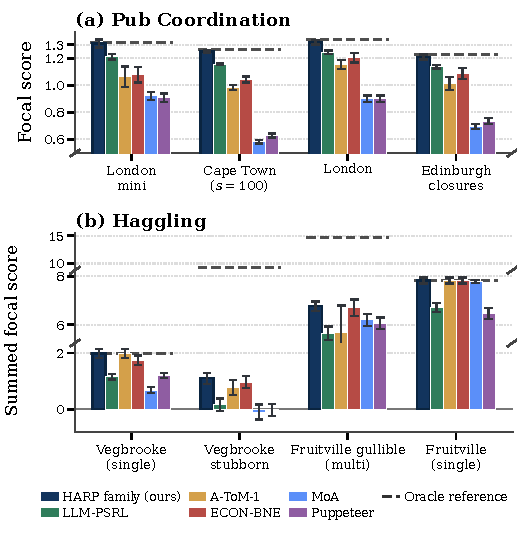
\includegraphics[width=\columnwidth]{figs/fig2_concordia_select_v15.pdf}
  \caption{Focal-agent payoff on the Concordia substrates. \emph{(a)} Pub Coordination, with \texttt{oracle\_joint} as the reference. \emph{(b)} Haggling, with the exact \texttt{oracle\_focal} as the reference and a broken vertical axis. Whiskers are standard errors over seeds; LLM-PSRL pools the four backbone--seed cells ($n{=}120$, or $400$ for Cape Town), while the mechanistic methods use the common $30$ seeds ($100$ for Cape Town).}
  \label{fig:concordia-main}
\end{figure}


\paragraph{RQ2 and RQ3: iterated diagnostic.} The one-shot format cannot show whether updating helps, because a single decision leaves nothing to update from. We therefore run a fixed-persona variant that updates across $K{=}20$ scenes on six held-out configurations, keeping the payoffs external and the geometries heterogeneous so that the resulting signatures reflect the inference machinery rather than our design. The paired difference between HARP and an explicit joint tracker covers zero within every geometry (Figure~\ref{fig:iterated-concordia}(a)), reproducing the parity of RQ2 on payoffs we do not control. The value of updating scales with how much the persona actually decides, from nothing on Pub Coordination to $1.1$--$1.7$ regret units on Haggling (b), and HARP\textsuperscript{+} reaches $0.352\pm0.035$ regret at a late rate of $0.0020$ against $1.361\pm0.172$ and $0.0764$ for PSRL-NoType. On the native one-shot format HARP and HARP\textsuperscript{+} coincide exactly, since a single decision leaves the bonus nothing to sharpen (Appendix Table~\ref{tab:bonus-ablation}). Updating is therefore the component that repetition rewards, and its value tracks how decision-relevant the persona is.

\begin{figure}[H]
  \centering
  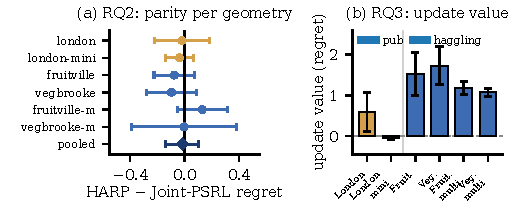
\includegraphics[width=0.92\columnwidth]{figs/fig_e_b_iterated_concordia_v5.pdf}
  \caption{Iterated Concordia over $K{=}20$ scenes on six held-out configurations, $5$ common seeds, under backbone-invariant exact-payoff replay. \emph{(a)} Paired HARP minus Joint-PSRL regret for each geometry and pooled, where negative values favor HARP. Whiskers are $t$-based $95\%$ intervals with $4$ degrees of freedom. \emph{(b)} Update value, the paired excess of PSRL-NoType over HARP\textsuperscript{+}, compared directly across configurations. Bars are the standard error of the mean.}
  \label{fig:iterated-concordia}
\end{figure}




\subsection{Case Study: Ride-Hailing Dispatch on MaaSSim}
\label{sec:maassim}

The first two substrates abstract coordination to a payoff table. To test the method in a setting closer to deployment, we replay MaaSSim, an agent-based ride-hailing simulator~\citep{kucharski2022simulating} with request queues, routing, and drivers who decline work they do not want. A dispatcher routes ride requests to independent drivers and each driver decides whether to accept, so the coordinator of Section~\ref{sec:algorithm} becomes the dispatcher and the LLM agents become the drivers. A driver's persona is a combination of four binary acceptance rules, giving $|\Theta_i|{=}16$ personas per driver, and the dispatcher never sees these rules. It observes only which offers each driver accepts or declines, so evidence about a persona arrives only for the offers that driver is actually routed, and a driver who is routed nothing reveals nothing. We replay from saved queue snapshots and persona maps rather than resimulating, which holds request arrivals and routing dynamics fixed across methods, so any difference in realized utility is attributable to belief quality alone. All runs use a single pinned backbone (Appendix~\ref{app:maassim}).

\paragraph{RQ1: margin under conflict.} Personas matter more when drivers disagree about which offers are acceptable, so we interpolate between the original replay and a transformation that makes acceptance rules maximally divergent, at $\lambda\in\{0,0.5,1\}$ and reject penalty $5$. The advantage of HARP over the strongest in-prompt baseline grows by roughly an order of magnitude across this sweep (Figure~\ref{fig:maassim-main}(a), with per-cell values in Appendix~\ref{app:maassim}). HARP stays within $2.7$--$4.4$ oracle-regret units throughout, while the strongest in-prompt baseline rises from $4.5$ to about $10.7$ (b). The gain therefore widens precisely where the persona carries more of the decision.

\paragraph{RQ2: parity at deployment scale.} Here the evidence is endogenous and censored, since a driver reveals its rule only through the offers it is routed, and the persona library has $|\Theta_i|{=}16$ rule combinations rather than four. We run an explicit joint tracker over the same event streams at $n\in\{2,3,4\}$ and compare it against the factored tracker directly. The two match to $2.5{\times}10^{-14}$ in marginal total variation, and their paired utility gap covers zero on five of six cells (Figure~\ref{fig:maassim-rq2}(a)). Coupling the prior across agents makes the joint posterior worth about a fifth of the regret, and pooling the same per-agent marginals within the coupled block recovers all of it at unchanged storage (Appendix~\ref{app:why-joint}). Update work here is measured rather than counted, at $497\,\mu$s per event for the joint tracker against a flat $7\,\mu$s for the factored one by $n{=}4$ (b), and the joint table becomes unrepresentable before the full population is reached, since $16$ rules across the deployed number of drivers exceeds any feasible table. Parity therefore holds where the explicit alternative stops being an option.

\paragraph{RQ3: identity, update, and dispatch.} To locate the source of the gain we vary where the dispatcher's belief comes from, holding the replay fixed. Realized utility rises with the accuracy of that belief (Figure~\ref{fig:maassim-rq2}(c)), and the learned posterior adds $+16.5$ utility over the prior, whereas equally sharp beliefs attached to the wrong drivers fall below it. The Concordia mode comparison agrees, with centralized dispatch accumulating regret $3$--$4\times$ more slowly than independent prompting (Appendix~\ref{app:decent-extended}). As on one-shot Concordia and the analytic ablation, rejections reveal type quickly enough that the bonus has nothing to sharpen, so it stays inactive as predicted, changing $4$ of $406$ assignments with a paired gap covering zero ($-0.25$, $95\%$ CI $[-0.81,0.31]$, Appendix Table~\ref{tab:bonus-ablation}). The belief itself forms from ordinary operational signal, concentrating well above chance within a handful of observations per driver (Appendix Figure~\ref{fig:maassim-concentration}), and rejections carry $1.7\times$ the per-event posterior gain of acceptances (Figure~\ref{fig:maassim-rq2}(d)), since all four hidden rules act as rejection triggers. What the dispatcher gains therefore comes from knowing which driver holds which rule, not from holding a belief at all.

\begin{figure}[H]
  \centering
  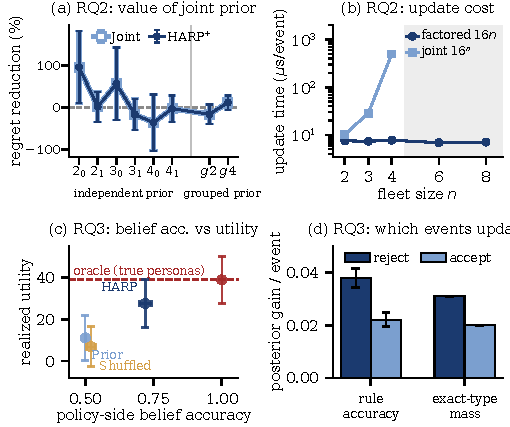
\includegraphics[width=\columnwidth]{figs/fig_maassim_rq23_v9.pdf}
  \caption{MaaSSim parity and mechanism. \emph{(a)} Relative reduction in oracle regret from tracking the joint persona posterior, as a percentage of the factored tracker's regret, with HARP\textsuperscript{+} coinciding pointwise. The left block keeps the persona prior independent across drivers ($10$ common environment seeds); the right block replaces it with shift groups of size $g$ sharing a persona, holding queue snapshots, routing, likelihood, and oracle fixed ($40$ seeds, common random numbers). \emph{(b)} Per-event update time, where the joint cost grows with the $16^{n}$ table and is not run beyond $n{=}4$. \emph{(c)} Realized utility against the accuracy of the belief the dispatcher acts on, over the belief sources of Figure~\ref{fig:maassim-main}(c), with the red dashed line marking the oracle on the true personas. The variants share common saved states, so paired contrasts are tighter than the marginal error bars shown. \emph{(d)} Per-event posterior gain by event type, over $279$ rejections and $388$ acceptances. Error bars are standard errors of the mean.}
  \label{fig:maassim-rq2}
\end{figure}


\section{Conclusion}
\label{sec:conclusion}
This paper introduces HARP, a novel framework that orchestrates heterogeneous LLM agents from an explicit persona posterior kept outside the prompt. A coordinator holds one numeric posterior per agent, samples a joint profile, plans centrally, and updates each marginal in closed form, so the language model supplies likelihoods and actions but never stores the belief. Under three structural conditions the per-agent posteriors reconstruct the joint one exactly, which reduces storage and update work from $O(|\Theta_i|^n)$ to $O(n|\Theta_i|)$ at unchanged regret, and bounded violations degrade the guarantee rather than void it.

The case is empirical. Under a control that fixes the persona profile, prior, payoffs, and exact optimum across methods, HARP\textsuperscript{+} attains the lowest regret of any non-oracle method on all four backbones, and the factored tracker matches explicit joint inference within seed-level error at up to $51\times$ smaller storage. The two remain identical to $n{=}8$ analytically, past the point at which the joint table exhausts memory, while the update stays flat at a few microseconds. Concordia reproduces the same separation on externally fixed payoffs and ties the value of updating to how much the persona actually decides, from nothing on venue coordination to over a regret unit on bargaining. MaaSSim carries the result into a dispatch replay, where the margin widens as competition for the same orders increases, at agent counts for which an explicit joint table is infeasible. Across substrates the gain requires the belief to be updated, to be attached to the agent it describes, and to be acted on by a single planner, and the discrimination bonus contributes wherever personas are slow to separate. Since the tracker is analytic and issues no online model calls, the advantage comes from where the belief is kept rather than from spending more of the backbone on it.

\section*{Limitations}
HARP assumes a fixed discrete persona library, a finite action space, and an outcome scorer calibrated offline, so continuous actions and personas that drift during an interaction remain open. The factorization compresses the belief but leaves the planner untouched, so centralized planning over the joint action space still bounds scale. Our substrates also impose the three structural conditions by construction, so the guarantees are claimed within that class rather than for social interaction in general, and open-ended dialogue is reported separately (Appendix~\ref{app:sotopia-detail}).

% Acknowledgments: add for camera-ready / non-anonymous venue.
% \section*{Acknowledgments}
% We thank ... for ... . This work was supported by ... .


% aaai2027.sty sets \bibliographystyle{aaai2027} automatically when natbib is
% loaded; declaring it again here causes bibtex's "Illegal, another \bibstyle".
\clearpage % references start after the seven-page main text
\bibliography{ref}

% Toggle: \withappendixtrue builds the submission PDF (7pp content + references
% + reproducibility checklist); \withappendixtrue additionally bundles the
% technical appendix (for the supplementary upload, split as required by AAAI-27).
\newif\ifwithappendix
\withappendixtrue

\ifwithappendix
\clearpage % page-exact boundary for extracting the supplementary PDF; this branch is excluded from the submission build
\appendix
\section{Empirical Supplement by Research Question}
\label{app:experiment-supplement}
\setcounter{subsection}{-1}

\subsection{Reading Guide}
\label{app:inventory}

This subsection certifies no standalone result; it maps each main-text research question to its complete evidence bundle and location. Claim tags C1--C6 name the certified claims within each question. Every empirical figure and table retained below appears in one of these rows, with the single exception of Appendix~\ref{app:oracles}, whose figures and table document the oracle references and the one-shot decision-quality comparison as shared evaluation infrastructure.

\begin{table}[h!]
\centering\scriptsize
\caption{Research-question reading guide. The appendix mirrors the main-text organization by research question.}
\label{tab:appendix-inventory}
\setlength{\tabcolsep}{1pt}
\begin{tabular}{@{}p{0.14\columnwidth}>{\raggedright\arraybackslash}p{0.58\columnwidth}p{0.22\columnwidth}@{}}
\toprule
Question & Evidence & Location \\
\midrule
\textbf{RQ1} representation & C1 matched control: Table~\ref{tab:hp-spgg-matched}; Figures~\ref{fig:e1-1-analytic},~\ref{fig:e1-1-llm}. C5 open-text boundary: Figure~\ref{fig:sotopia-main}; Tables~\ref{tab:sotopia-pf-families},~\ref{tab:sotopia-aggregate}; Figures~\ref{fig:sotopia-corrected},~\ref{fig:sotopia-component-corrected}; Table~\ref{tab:sotopia-corrected}. & \S\ref{app:llm-supplements} \\[2pt]
\textbf{RQ2} computation & C1 exactness/storage: Figure~\ref{fig:storage-vs-regret}; Tables~\ref{tab:storage-comparison},~\ref{tab:maassim-parity},~\ref{tab:maassim-grouped-prior}; Figure~\ref{fig:maassim-rq2}(a,b). C4 structural class: Figure~\ref{fig:rl-violation}; Table~\ref{tab:rl-violation}; Figure~\ref{fig:e1-3-pf}; Table~\ref{tab:true-shared-dgp}. & \S\ref{app:hp-spgg-diagnostics} \\[2pt]
\textbf{RQ3} attribution & C2 rate: Figures~\ref{fig:e2-e5}(a),~\ref{fig:app-e2-native},~\ref{fig:iterated-concordia}; Table~\ref{tab:iterated-concordia}. C3 bonus: Figure~\ref{fig:e2-e5}(b); Figures~\ref{fig:n-scaling},~\ref{fig:beta-sweep}; Table~\ref{tab:bonus-ablation}. C6 mechanism: Figures~\ref{fig:component-ladder},~\ref{fig:decentralized-price},~\ref{fig:maassim-rq2}(c,d),~\ref{fig:maassim-concentration},~\ref{fig:maassim-mechanism},~\ref{fig:maassim-tradeoff}; Tables~\ref{tab:maassim-mechanism},~\ref{tab:maassim-scenarios}; Figures~\ref{fig:maassim-conflict-dynamics},~\ref{fig:maassim-unit-validation}. & \S\ref{app:rate-burnin} \\
\bottomrule
\end{tabular}
\end{table}

\subsection{RQ1: Numeric versus In-Prompt Representation}
\label{app:llm-supplements}

This subsection certifies where the representational advantage is measured (C1's environment-matched control) and where it stops (C5's open-text boundary).

\subsubsection{Environment-Matched Control (C1)}

\paragraph{Matched-likelihood source audit.}
\label{app:matched-likelihood-audit}
Git snapshot \texttt{4280ade} used algorithm-specific seeds ($120000+10000j+s$) and did not retain its c19 tensors or response caches, so those historical unmatched rows are provenance only and are excluded from Figure~\ref{fig:hp-spgg-cross-model} and Table~\ref{tab:hp-spgg-matched}.
\paragraph{Fresh environment-matched control.}
For each backbone we generated and pinned a complete $125$-profile ${\times}\,3$-player ${\times}\,4$-persona live outcome-score tensor (1,500 judge cells), then ran all methods over the same ten environment seeds, type profiles, uniform prior, and exact exhaustive tensor oracle with $K{=}20$, $\beta{=}0.25$, and Gaussian observation scale $0.08$. There is no additional stochastic board state. Each method receives its own realized-reward history generated from the shared tensor. The strongest fixed LLM-coordination comparator is selected by minimum mean regret within ECON-BNE and A-ToM-0/1/2. Ratios divide per-backbone means; paired gaps use common seed indices. Provider sampling seeds are unavailable, so this is environment matching rather than pathwise provider-RNG matching; every accepted raw response is content-hash cache-pinned. The final column is reported as a sanity check that the method exploits the structure when it is present, not as a separate claim: HP-SPGG is constructed so that TI, RL, and PF hold and the persona-conditioned outcome scorer is exactly calibrated, which is precisely the regime the method targets and the prompt-based comparators do not assume. The spread across backbones is driven by the comparators rather than by HARP\textsuperscript{+}: its own regret varies by a factor of $2.7$ ($0.159$ to $0.430$) while the strongest prompt-based comparator varies by $9.9$ ($0.700$ on Llama-Maverick to $6.960$ on GPT-5.4-nano), and the two extremes fall on opposite backbones. This is the behavior the design predicts, since a belief kept numeric and outside the prompt, updated against a outcome scorer calibrated once per backbone, inherits little of the variation in a backbone's in-context reasoning quality. We therefore report the range rather than a single headline multiple, and read the Llama cell as one where a prompt-based comparator happens to do well rather than one where HARP\textsuperscript{+} degrades. The claims certified in this subsection are the exactness and storage results below.

\begin{table*}[t]
\centering\scriptsize
\caption{Environment-matched HP-SPGG control ($K{=}20$, $10$ common seeds). Values are cumulative regret, mean $\pm$ SEM. Ratio is the strongest fixed LLM-coordination baseline divided by the lower-regret HARP-family member (HARP\textsuperscript{+} on all four backbones).}
\label{tab:hp-spgg-matched}
\setlength{\tabcolsep}{3pt}
\begin{tabular}{lrrrrlr}
\toprule
Backbone & HARP\textsuperscript{+} & HARP & Joint-PSRL & LLM-PSRL & Best coordination & Coord./best HARP \\
\midrule
DeepSeek-V3.2 & $0.360\pm0.142$ & $0.985\pm0.298$ & $0.955\pm0.203$ & $18.270\pm5.141$ & ECON-BNE $2.550\pm1.049$ & $7.08\times$ \\
GPT-5.4-nano & $0.159\pm0.038$ & $0.544\pm0.150$ & $0.391\pm0.100$ & $2.193\pm0.714$ & ECON-BNE $6.960\pm1.376$ & $43.77\times$ \\
Kimi-K2.6 & $0.325\pm0.088$ & $0.547\pm0.116$ & $0.642\pm0.159$ & $6.701\pm1.325$ & ECON-BNE $2.957\pm1.366$ & $9.10\times$ \\
Llama-4-Maverick & $0.430\pm0.217$ & $1.202\pm0.212$ & $1.276\pm0.228$ & $13.510\pm3.431$ & A-ToM-0 $0.700\pm0.396$ & $1.63\times$ \\
\bottomrule
\end{tabular}
\end{table*}
\paragraph{HP-SPGG state, action, and calibration specification.}
The public state at each turn records the round index and the previous turn's realized contribution profile. Each agent's action menu is the discrete contribution grid $\mathcal A_i$ with five levels, so the joint menu contains $5^3{=}125$ profiles that the backward-induction planner and the oracle both enumerate exactly ($\epsilon_{\mathrm{plan}}{=}0$). Persona-conditioned rewards are calibrated offline once per backbone by scoring every (persona, player index, contribution profile) cell with the judge prompt of Section~\ref{app:prompt-hp-spgg-scoring}, yielding the $125\times3\times4$ tensor that serves as both the planner's outcome scorer and the mean of the tracker's likelihood. The observation likelihood is the calibrated Gaussian factor with scale $\sigma{=}0.08$ given below Eq.~\eqref{eq:likelihood}, and the action factor is uninformative, so the online tracker issues no model calls. All reported cells use $K{=}20$ episodes, $n{=}3$ agents, $|\Theta_i|{=}4$ personas, and $\beta{=}0.25$.
\paragraph{Baseline definitions.}
\emph{Oracle} receives the true persona profile and applies the same exhaustive joint-action argmax, providing the regret reference. \emph{HARP} and \emph{HARP\textsuperscript{+}} share every component and differ only in the bonus weight $\beta$. \emph{Joint-PSRL} replaces the factored persona posterior with an explicit table over all $|\Theta_i|^n$ joint profiles under a uniform Dirichlet prior while sharing the likelihood, planner, and environments. \emph{LLM-PSRL} retains the posterior-sampling loop but represents the hypothesis and posterior in natural language rather than numerically. \emph{PSRL-NoType} draws $\hat{\boldsymbol\theta}\sim\mathrm{Unif}(\Theta)$ each episode and never updates. \emph{A-ToM-0/1/2} apply adaptive theory-of-mind prompting at three recursion levels \citep{mu2026adaptive} and \emph{ECON-BNE} applies debate-of-beliefs equilibrium reasoning \citep{yi2025debate}; both keep their belief state inside the prompt and receive realized rewards from the same pinned tensor through their public history.

\subsubsection{Open-Text Transfer Boundary (C5)}
\label{app:sotopia-detail}

This subsection certifies C5: once actions are open-ended and TI/RL/PF cannot be verified, the exact finite-model guarantees no longer transfer, and correcting the recurrent evidence path produces no focal-score gain.

\paragraph{Setup recap.} SOTOPIA-Hard \citep{zhou2024sotopia} sits outside HT-MG's preconditions on three axes. The substrate is dyadic ($n{=}2$) rather than $n\!\geq\!3$, the action space is open-ended natural language rather than tabular contributions, and episodes are curated profile-goal pairs rather than samples from an explicit factored prior, so (TI), (RL), and (PF) are not verified in either direction. We adapt HARP\textsuperscript{+} by extracting approximate per-agent persona marginals from a Concordia-style mechanistic surrogate over a discretized intent space, then apply the same factored-posterior sampling and type-discrimination bonus as in HP-SPGG. The surrogate scores each utterance with fixed keyword-weighted heuristics over the intent menu rather than next-token likelihoods, and the reference one-hot labels are obtained by applying the same mapping to the full profile. An implementation audit conducted before submission found that the evidence channel of the original runs read from the agent inbox while SOTOPIA 0.1.5 delivers partner evidence in \texttt{Observation.last\_turn}, so the numeric posterior in those runs received zero updates and the tracker acted as prior sampling. We therefore treat all historical SOTOPIA-Hard numbers as descriptive results produced by the intent surrogate, the type-discrimination bonus, and prior sampling, and we do not use them to support the closed-form belief-update mechanism. The corrected recurrent rerun is reported in Section~\ref{app:sotopia-corrected}. Both agents in each episode are controlled by the same baseline (Sotopia self-play). The focal score is the mean of \texttt{episode.overall.agent\_1} and \texttt{episode.overall.agent\_2}. We compare against four LLM-coordination baselines, A-ToM-1 \citep{mu2026adaptive}, ECON-BNE \citep{yi2025debate}, prompted \texttt{llm\_belief}, and prompted \texttt{llm\_greedy}. Each (backbone, baseline) cell is averaged over $14$ scenarios with $5$ seeds each, for $70$ episodes per cell.

\begin{figure*}[t]
  \centering
  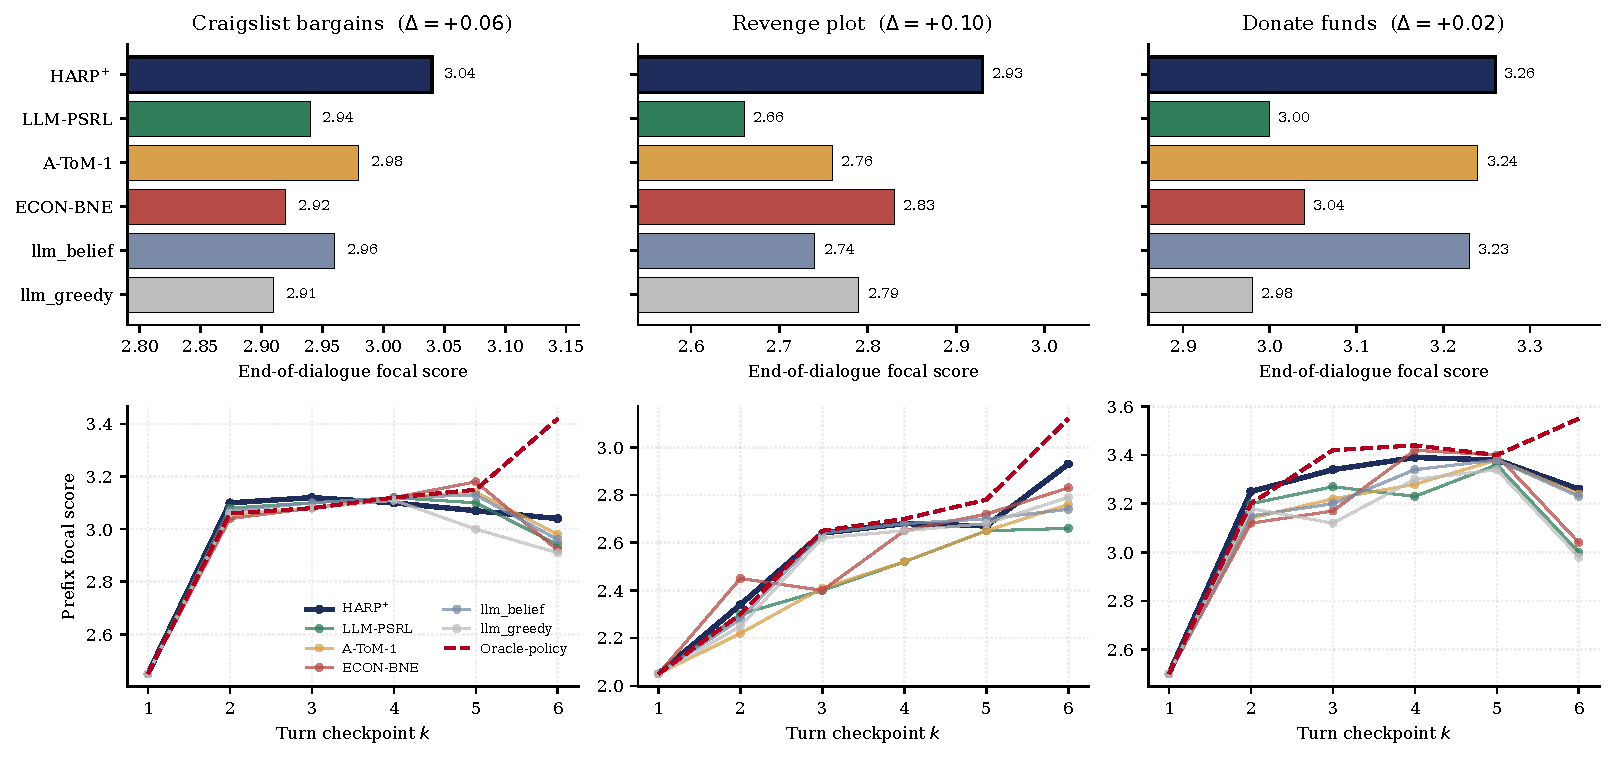
\includegraphics[width=0.985\textwidth]{figs/fig_sotopia_combined_v7.pdf}
  \caption{SOTOPIA-Hard descriptive results for three private-goal families: \emph{craigslist\_bargains} ($n{=}80$), \emph{revenge\_plot} ($n{=}20$), and \emph{donate\_funds} ($n{=}20$). \emph{(a)} End-of-dialogue focal score across four backbones (SEM); $\Delta$ compares HARP\textsuperscript{+} with the next-best LLM-coordination baseline. \emph{(b)} Prefix-only per-turn trajectory (descriptive; the historical tracker did not update, so this panel is not concentration evidence); red dashed is \texttt{oracle\_policy} (Appendix~\ref{app:oracle-construction}).}
  \label{fig:sotopia-main}
\end{figure*}

\paragraph{Historical descriptive results.} Figure~\ref{fig:sotopia-main} and Table~\ref{tab:sotopia-pf-families} report the three private-goal families summarized in the main text. HARP\textsuperscript{+} ranks between second and fourth by backbone, every method falls inside a $0.12$ envelope of focal score, and the family margins are $+0.06$, $+0.10$, and $+0.02$. Because the retained tracker did not update, these margins describe the intent surrogate, prior sampling, and bonus configuration rather than recurrent Bayesian inference.

\begin{table}[h]
\centering\small
\caption{SOTOPIA-Hard private-goal families: HARP\textsuperscript{+} vs.\ strongest LLM-coordination baseline per family, averaged across four backbones. Best baseline per family: A-ToM-1 for \emph{craigslist\_bargains} and \emph{donate\_funds}; ECON-BNE for \emph{revenge\_plot}.}
\label{tab:sotopia-pf-families}
\setlength{\tabcolsep}{6pt}
\begin{tabular}{@{}lcccc@{}}
\toprule
Family & $n$ & HARP\textsuperscript{+} & Best & $\Delta$ \\
\midrule
craigslist\_bargains & 80  & 3.04 & 2.98 & +0.06 \\
revenge\_plot        & 20 & 2.93 & 2.83 & +0.10 \\
donate\_funds        & 20  & 3.26 & 3.24 & +0.02 \\
\bottomrule
\end{tabular}
\end{table}

\paragraph{Aggregate scores and interpretation.} Table~\ref{tab:sotopia-aggregate} reports mean focal score by backbone. HARP\textsuperscript{+} ranks 2nd/3rd/3rd/4th on GPT/DeepSeek/Kimi/Llama and remains within $0.10$ of the best alternative; all five non-oracle methods fit inside a $0.12$ envelope. The one-hot \texttt{oracle\_belief} row also lies within that envelope on average, whereas best-of-five \texttt{oracle\_policy} reaches $3.540$. Thus open action search and judge variance dominate the value of the surrogate persona belief. Because TI/RL/PF are unverified and the tracker was static, these historical rows certify a transfer boundary, not a rate or concentration claim.

\begin{table*}[h]
\centering\small
\caption{SOTOPIA-Hard aggregate mean focal score per (backbone $\times$ baseline), $70$ episodes per cell. \textbf{Bold} marks the highest non-oracle score per backbone; HARP\textsuperscript{+} rank and gap to best alternative are in the last two columns. The two oracle rows (Appendix~\ref{app:oracle-construction}) receive the privileged one-hot opponent persona; \texttt{oracle\_policy} additionally selects the best of $K{=}5$ independent episodes by the same seven-dimensional judge.}
\label{tab:sotopia-aggregate}
\begin{tabular}{lccccccc}
\toprule
Backbone & HARP\textsuperscript{+} & A-ToM-1 & ECON-BNE & llm\_belief & llm\_greedy & Rank & $\Delta$ \\
\midrule
DeepSeek-V3.2 & 3.248 & 3.261 & \textbf{3.313} & 3.195 & 3.193 & 3 & $-0.065$ \\
GPT-5.4-nano & 2.981 & 2.918 & 2.843 & \textbf{3.000} & 2.842 & 2 & $-0.019$ \\
Kimi-K2.6 & 2.807 & 2.733 & 2.876 & \textbf{2.906} & 2.761 & 3 & $-0.099$ \\
Llama-Maverick & 3.308 & \textbf{3.359} & 3.319 & 3.340 & 3.165 & 4 & $-0.051$ \\
\midrule
\emph{Average} & 3.086 & 3.068 & 3.088 & \textbf{3.110} & 2.990 & --- & $-0.024$ \\
\bottomrule
\end{tabular}

\vspace{4pt}
\begin{tabular}{lcc}
\toprule
Backbone & \texttt{oracle\_belief} (one-hot persona) & \texttt{oracle\_policy} (one-hot + best-of-$K{=}5$) \\
\midrule
DeepSeek-V3.2 & 3.294 & 3.712 \\
GPT-5.4-nano  & 2.920 & 3.467 \\
Kimi-K2.6     & 2.916 & 3.364 \\
Llama-Maverick & 3.282 & 3.618 \\
\midrule
\emph{Average} & 3.103 & 3.540 \\
\bottomrule
\end{tabular}
\end{table*}

\paragraph{Corrected recurrent tracker.}
\label{app:sotopia-corrected}

We repaired the adapter to read partner evidence from SOTOPIA 0.1.5's \texttt{Observation.last\_turn}. A corrected GPT-5.4-nano run covers the same three private-goal families with $120$ episodes at each corruption level; every accepted episode records eligible recurrent updates and zero provider-exception generation fallbacks. This run is separate from the historical four-backbone results above.

SOTOPIA provides no native labels for the project's four persona classes. Figure~\ref{fig:sotopia-corrected}(a) therefore evaluates concentration only against the existing \emph{profile-derived proxy} used by the oracle adapter. Proxy mass rises from $0.25$ to $0.304\pm0.012$ on \emph{revenge\_plot}, but falls to $0.233\pm0.005$ on \emph{craigslist\_bargains} and changes only to $0.261\pm0.013$ on \emph{donate\_funds}. The corrected tracker is recurrent and nontrivial, but concentration is family-dependent and is not native type-recovery accuracy.

The corrected $p{=}0$ focal means are $2.665\pm0.074$, $3.229\pm0.121$, and $2.743\pm0.102$ on \emph{craigslist\_bargains}, \emph{donate\_funds}, and \emph{revenge\_plot}. They trail the retained GPT-nano best-baseline means by $0.095$, $0.157$, and $0.457$, respectively. We therefore select the clean-boundary branch: fixing the evidence path removes the implementation liability but does not produce a score advantage. Figure~\ref{fig:sotopia-corrected}(b) reports the completed measured grid $p\in\{0,0.1,0.2,0.25,0.3,0.5\}$; no point is interpolated. At $p{=}0.5$, changes from $p{=}0$ are $-0.053$, $+0.161$, and $+0.146$ across the three families. The curve is non-monotone and changes are comparable to episode-row SEM, so it supports sensitivity bounds rather than a causal degradation law.

\begin{figure*}[t]
  \centering
  
\includegraphics[width=0.84\textwidth]{figs/fig_e_c_sotopia_corrected.pdf}
  \caption{Corrected SOTOPIA tracker diagnostic on GPT-5.4-nano. \emph{(a)} Recurrent mass on the profile-derived proxy persona (not a native SOTOPIA truth label); error bars are episode-row SEM. \emph{(b)} Focal score under deterministic intent-menu corruption; provider and judge generations are not pathwise seed-controlled, so this is a sensitivity bound rather than a paired causal dose response.}
  \label{fig:sotopia-corrected}
\end{figure*}

\begin{table}[h]
\centering\small
\caption{Corrected $p{=}0$ SOTOPIA branch decision. Historical best is the retained GPT-nano comparator, not a contemporaneous paired rerun.}
\label{tab:sotopia-corrected}
\begin{tabular}{lrr}
\toprule
Family & Corrected score & $\Delta$ vs best \\
\midrule
Craigslist & $2.665\pm0.074$ & $-0.095$ \\
Donate & $3.229\pm0.121$ & $-0.157$ \\
Revenge & $2.743\pm0.102$ & $-0.457$ \\
\bottomrule
\end{tabular}
\end{table}

\paragraph{Corrected component controls.} We rerun surrogate-only, naive-belief, and HARP\textsuperscript{+} on the same $30$ cases and four replicate IDs. The endpoint exposes no sampling-seed control, so pairing controls case composition but not provider or judge randomness. HARP-minus-naive paired differences are $+0.044\pm0.096$, $+0.093\pm0.182$, and $-0.043\pm0.150$ on Craigslist, Donate, and Revenge; HARP-minus-surrogate differences are $+0.063\pm0.077$, $-0.079\pm0.090$, and $-0.107\pm0.166$. No lower confidence bound is positive. Together with the corrected recurrent updates, this selects the clean-boundary branch: the tracker functions, but no focal-score gain can be attributed to its numeric update on these families.

\begin{figure}[h]
  \centering
  
\includegraphics[width=0.95\columnwidth]{figs/fig_e_c_sotopia_component_corrected.pdf}
  \caption{Corrected SOTOPIA component variants on GPT-5.4-nano (same $30$ cases, four replicates; episode-row SEM). HARP\textsuperscript{+} does not significantly exceed either corrected control on any family. Provider generations are not pathwise seed-controlled.}
  \label{fig:sotopia-component-corrected}
\end{figure}


\subsection{RQ2: Factored versus Joint Computation}
\label{app:hp-spgg-diagnostics}

\subsubsection{Exactness and Storage (C1)}

This unit certifies C1: under TI/RL/PF, the factored persona posterior matches the joint representation while reducing persona storage from $O(|\Theta_i|^n)$ to $O(n|\Theta_i|)$. The matched control of Section~\ref{app:llm-supplements} anchors the comparison on common environments and pinned tensors; the scaling figures and storage table isolate representation size from planning and likelihood differences.



\paragraph{HARP--Joint agreement.}
In Table~\ref{tab:hp-spgg-matched}, the absolute HARP--Joint-PSRL mean-regret gaps are $0.030$, $0.153$, $0.095$, and $0.074$ across DeepSeek, GPT, Kimi, and Llama; each is smaller than the corresponding quadrature-combined SEM. This aggregate agreement is consistent with Proposition~\ref{prop:bit-identical}. The live control does not claim trajectory identity because algorithm draws were not pathwise coupled and the provider-sampled calibration exposes no replayable sampling seed, instead pinning one realized tensor by cache.
\paragraph{Representation-only comparison.}
Figures~\ref{fig:e1-1-analytic} and~\ref{fig:e1-1-llm} broaden the agent-count sweep to nine baselines. Under the structural conditions, HARP and the explicit joint-posterior sampler remain within sample noise while type-agnostic IQL and Random accumulate regret with $n$. Table~\ref{tab:storage-comparison} holds the likelihood, planner, and seeds fixed and changes only posterior representation; the storage ratio grows from $5.3\times$ to $51\times$ over $n=3$--$5$ without a corresponding regret separation. Figure~\ref{fig:storage-vs-regret} puts the two quantities on the same axes for one live backbone: the three posterior-sampling methods track one another in regret at every $n$ while the joint table grows from $16$ to $1024$ entries against HARP's $8$ to $20$, so the entire benefit of decoupling appears as storage rather than as a regret gap. This is the finite-sample form of Corollary~\ref{cor:storage}, and it also shows where the saving is not yet worth anything: at $n{=}2$ the joint table has only $16$ entries, the ratio is $2.0\times$, and all three methods sit at the same elevated regret. Seed counts in Figure~\ref{fig:storage-vs-regret} are not uniform across cells: $n{=}2$ aggregates $10$ seeds and $n{=}3,4,5$ aggregate $5$ each, the $n{=}2$ cell having been re-run for outlier confirmation. The panel is a single-backbone (Llama-4-Maverick) view; the cross-backbone form of the same comparison is Table~\ref{tab:storage-comparison}.

\begin{figure}[t]
  \centering
  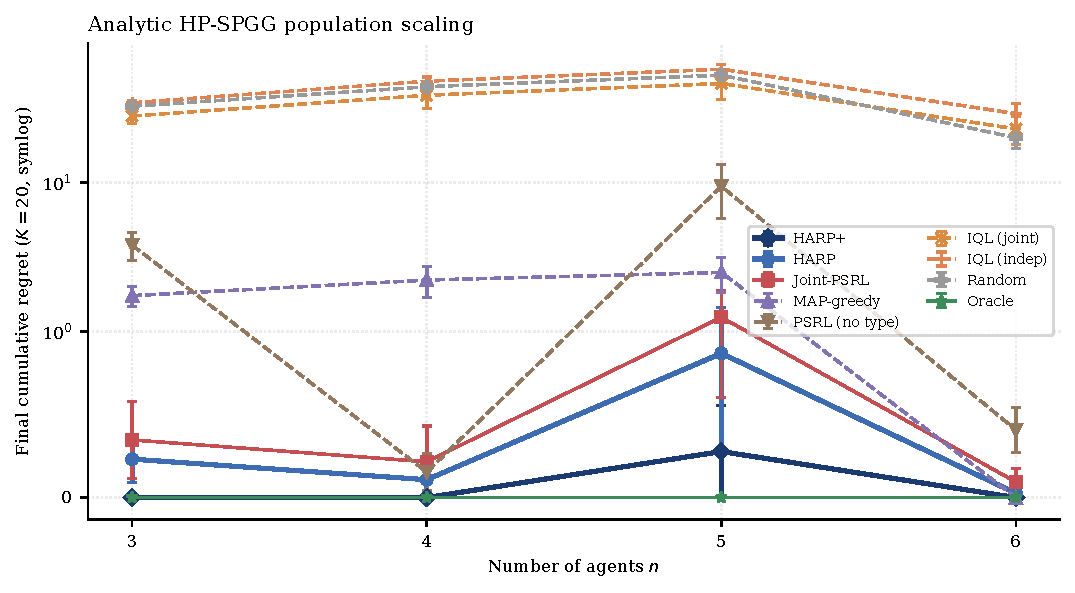
\includegraphics[width=\columnwidth]{figs/fig_e1_1_n_scaling.pdf}
  \caption{C1 analytic-tier nine-baseline $n$-scaling on HP-SPGG ($n\in\{3,4,5,6\}$, $K{=}20$, $5$ seeds, $\beta{=}0.25$). The HARP family stays under $1.0$ cumulative regret across the sweep while type-agnostic IQL and Random grow with $n$. Persona-storage savings are $5.3\times$, $16\times$, $51\times$, and $171\times$ at $n=3,4,5,6$.}
  \label{fig:e1-1-analytic}
\end{figure}

\begin{figure}[t]
  \centering
  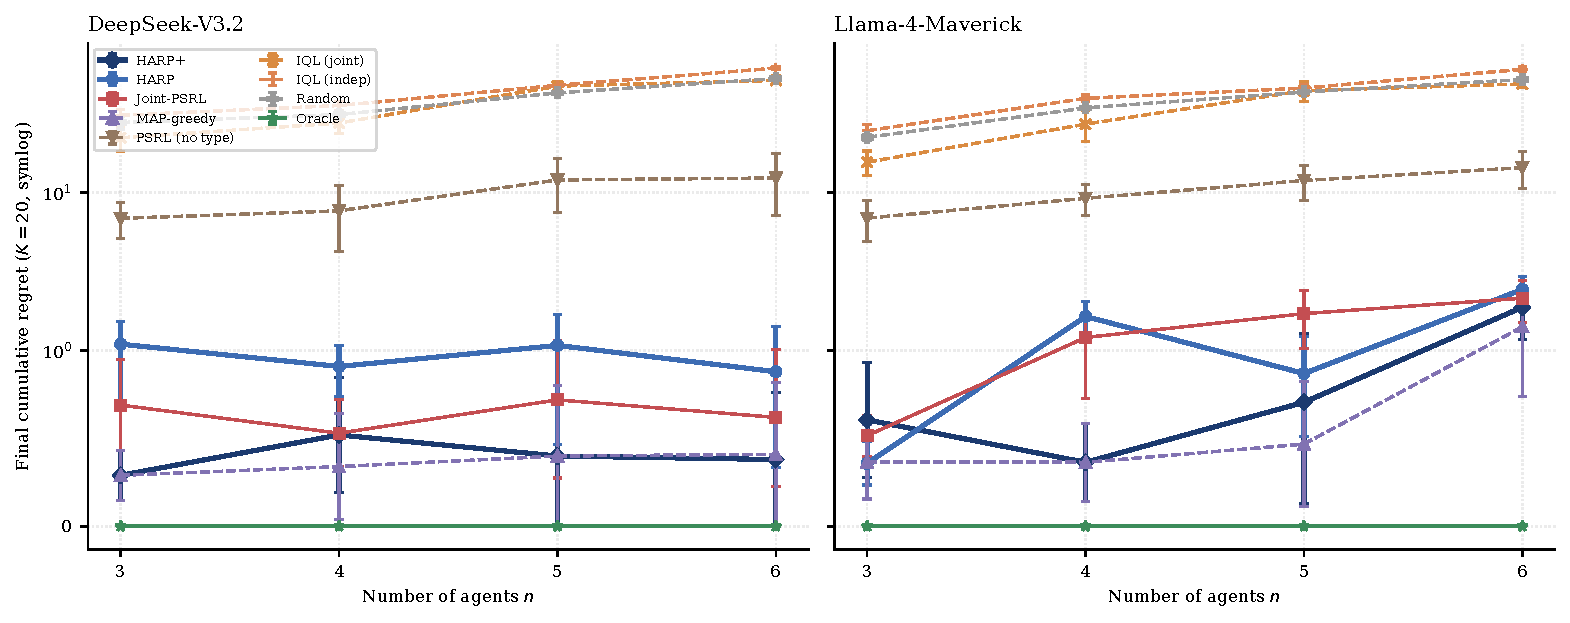
\includegraphics[width=\columnwidth]{figs/fig_e1_1_n_scaling_llm.pdf}
  \caption{C1 live-LLM nine-baseline $n$-scaling on HP-SPGG c19 ($K{=}20$, $5$ common environment seeds, $\beta{=}0.25$). Left: DeepSeek-V3.2. Right: Llama-4-Maverick. The HARP family remains separated from type-agnostic baselines on both backbones; external A-ToM-0/1/2 and ECON-BNE references are shown at $n{=}3$.}
  \label{fig:e1-1-llm}
\end{figure}

\begin{table}[t]
\centering\small
\caption{Factored-vs-joint storage comparison on HP-SPGG ($m{=}|\Theta_i|{=}4$, $K{=}100$, $10$ common environment seeds, $\beta{=}0.25$). HARP and Joint-PSRL-Uniform share likelihood, exhaustive planner, and seeds; only the posterior representation differs. Values are cumulative regret.}
\label{tab:storage-comparison}
\setlength{\tabcolsep}{4pt}
\begin{tabular}{@{}cccccc@{}}
\toprule
   & Storage & \multicolumn{2}{c}{analytic kernel} & \multicolumn{2}{c}{DeepSeek-V3.2} \\
\cmidrule(lr){3-4}\cmidrule(lr){5-6}
$n$ & savings & HARP & J-PSRL-U & HARP & J-PSRL-U \\
\midrule
3 & 5.3$\times$ & 0.12 & 0.17 & 0.57 & 0.38 \\
4 & 16$\times$  & 0.05 & 0.11 & 0.80 & 0.51 \\
5 & 51$\times$  & 0.60 & 0.63 & 1.02 & 0.85 \\
\bottomrule
\end{tabular}
\end{table}
\paragraph{MaaSSim parity control (E-E).}
The same exactness claim is tested on the deployment-shaped substrate. Closed-loop regeneration by fleet size produces sub-fleets of $n\in\{2,3,4,6,8\}$ drivers over the ten common environment indices at $\lambda\in\{0,1\}$, with the base driver-reject penalty of $2$ rather than the stress setting of the main-text sweep. Both trackers consume the identical nearest-policy saved assignment events in identical order, share the per-driver binary accept/reject analytic likelihood, the uniform prior, and an exhaustive maximum-cardinality assignment objective with lexicographic tie-breaking, and draw profiles from independent deterministic sampling RNG streams. The joint tracker maintains the explicit $16^{n}$ table and is run for $n\le4$; the $16^{8}$ table at the full fleet is infeasible for the experiment budget. Table~\ref{tab:maassim-parity} reports the six paired cells. Marginal total variation between the joint and factored posteriors stays at numerical precision on every stream, so the trackers are the same posterior in two representations, and any utility difference arises from the independent profile-sampling draws. One of six $95\%$ intervals excludes zero ($n{=}2$, $\lambda{=}0$); at least one excursion among six such intervals occurs with probability ${\approx}0.26$, the direction is not reproduced at any other cell, and the pooled mean over cells is $-0.01$. Per-event update cost is flat near $7\,\mu$s for the factored tracker at every fleet size and grows to $497\,\mu$s for the joint tracker at $n{=}4$ (Figure~\ref{fig:maassim-rq2}(b)).

\begin{table}[t]
\centering\scriptsize
\caption{E-E paired utility gap (joint $-$ factored; $10$ common environment seeds, mean and $95\%$ CI) and posterior identity.}
\label{tab:maassim-parity}
\setlength{\tabcolsep}{3.5pt}
\begin{tabular}{ccrcc c}
\toprule
$n$ & $\lambda$ & Gap & $95\%$ CI & Max TV & Entries \\
\midrule
$2$ & $0$ & $+1.85$ & $[+0.19,\,+3.51]$ & $7.8\times10^{-16}$ & $256$ vs $32$ \\
$2$ & $1$ & $+0.11$ & $[-2.87,\,+3.10]$ & $7.8\times10^{-16}$ & $256$ vs $32$ \\
$3$ & $0$ & $+1.33$ & $[-0.71,\,+3.37]$ & $2.5\times10^{-15}$ & $4096$ vs $48$ \\
$3$ & $1$ & $-1.59$ & $[-5.13,\,+1.95]$ & $2.5\times10^{-15}$ & $4096$ vs $48$ \\
$4$ & $0$ & $-1.38$ & $[-3.90,\,+1.15]$ & $2.5\times10^{-14}$ & $65536$ vs $64$ \\
$4$ & $1$ & $-0.37$ & $[-4.08,\,+3.34]$ & $2.5\times10^{-14}$ & $65536$ vs $64$ \\
\bottomrule
\end{tabular}
\end{table}

\paragraph{Grouped-prior control (E-H).}
\label{app:why-joint}
The parity result above assumes independently drawn driver personas. We also impose a grouped prior in which each group of $g$ drivers shares one latent persona, while retaining the same queue snapshots, deterministic hidden-rule responses, $16$-persona library, and exhaustive assignment objective. All samplers use common random numbers keyed by seed, round, and group. The discovery set (seeds $0$--$19$) gives a HARP-minus-Joint regret gap of $+0.7750\pm0.3691$ at $g{=}4$. Before generating any new outcomes, we preregistered seeds $20$--$59$, the paired endpoint, and its $t_{39}$ interval. The confirmatory gap is $+0.7865\pm0.3644$ with $95\%$ CI $[+0.0495,+1.5235]$. Joint therefore reduces mean oracle regret from $3.7823$ to $2.9958$, or $20.8\%$ relative to HARP. At $g{=}2$ the gap is unresolved and reverses in point estimate ($-0.5843\pm0.5697$); the preregistered paired group-size contrast, gap$_{g=4}-$gap$_{g=2}$, is $+1.3708\pm0.6020$ with CI $[+0.1531,+2.5884]$. Table~\ref{tab:maassim-grouped-prior} reports the complete comparison.

HARP-S pools the $g$ per-driver marginals before drawing one persona per group. It is pathwise identical to Joint under the uniform prior: action, utility, and regret mismatches are all $0/800$ under the deterministic indicator likelihood on confirmatory seeds $20$--$59$, and all $0/400$ under the softmax likelihood on discovery seeds $0$--$19$. Proposition~\ref{prop:uniform-group-pooling} shows that this equality holds for any conditionally factorized likelihood under a uniform prior, and identifies the repeated-prior correction required away from uniformity.

\begin{table}[t]
\centering\scriptsize
\caption{E-H grouped-prior control on confirmatory seeds $20$--$59$ ($n{=}8$, $m{=}2$, $K{=}20$, $\rho{=}1$). Regrets are means $\pm$ SEM; gaps use paired $t_{39}$ intervals. Relative reduction is $(\overline R_{\mathrm{HARP}}-\overline R_{\mathrm{Joint}})/\overline R_{\mathrm{HARP}}$.}
\label{tab:maassim-grouped-prior}
\setlength{\tabcolsep}{3pt}
\begin{tabular}{crrrr}
\toprule
$g$ & HARP regret & Joint $=$ HARP-S & HARP $-$ Joint & Relative \\
\midrule
$2$ & $4.6115\pm0.6576$ & $5.1958\pm0.7773$ & $-0.5843\pm0.5697$ & $-12.7\%$ \\
$4$ & $3.7823\pm0.6097$ & $2.9958\pm0.5692$ & $+0.7865\pm0.3644$ & $+20.8\%$ \\
\bottomrule
\end{tabular}
\end{table}

\subsubsection{Analytic Scaling to the Joint Feasibility Frontier}
\label{app:scaling}

A dedicated scaling suite extends the exactness and storage evidence to $n{=}10$ agents and a $16$-type library, entirely on the analytic tier with zero LLM calls. Three sweeps share $K{=}50$, ten common seeds ($1000$--$1009$), $\beta{=}0.25$, outcome noise $\sigma{=}0.08$, and the five-value action menu read from the substrate. A population sweep holds $|\Theta_i|{=}4$ and runs $n\in\{2,\dots,10\}$, a library sweep holds $n{=}3$ and runs $|\Theta_i|\in\{4,8,16\}$ with types synthesized on the archetype parameter grid, and a frontier sweep holds $|\Theta_i|{=}16$ and runs $n\in\{2,\dots,8\}$. The explicit joint tracker is ruled infeasible when its table exceeds $4$\,GB or a single update exceeds $1$\,s, and the shared planner enumerates at most $2^{24}$ joint profiles per step, a cap that never binds through the largest cell.

\paragraph{Exact parity at scale.} On every one of the $17$ joint-feasible cells, HARP and Joint-PSRL produce identical action sequences and identical regret trajectories, with maximum trajectory gap $0.0$ and zero action mismatches over $170$ seed-cells. Proposition~\ref{prop:bit-identical} therefore holds as measured fact up to a joint-to-factored storage ratio of $174{,}763\times$ at $(n{=}6,|\Theta_i|{=}16)$, where the joint table holds $16.8$M entries against the factored tracker's $96$. Per-event update work separates accordingly, growing from $7.5\,\mu$s at $n{=}2$ to $68.8$\,ms at $n{=}6$ for the joint tracker while HARP stays within $1.3$--$4.8\,\mu$s across every cell of every sweep.

\paragraph{The frontier, and what survives past it.} The joint tracker crosses the feasibility boundary inside the sweep. At $n{=}7$ its first update takes $1.02$\,s and the update-time rule fires, and at $n{=}8$ the $16^8$-entry table requires $34.4$\,GB and the memory rule fires. The factored methods continue unchanged. Table~\ref{tab:scaling-frontier} reports the frontier sweep. HARP\textsuperscript{+} remains within $0.06$ of the pinned oracle at $n{=}7$ and $n{=}8$, past the boundary where explicit joint inference cannot run, while PSRL-NoType accumulates $6.0$--$7.3$ with near-perfectly linear growth (slopes $0.07$--$0.15$ per episode, $R^2\ge0.998$ on every separating cell).

\paragraph{The bonus under a weakly discriminating library.} The synthesized $16$-type library has minimum pairwise Hellinger gap $\hat\rho=1.2\times10^{-3}$, so identification is slow even with exact likelihoods, and the discrimination bonus carries the burn-in exactly as Proposition~\ref{prop:misspec-contraction} predicts for a small effective gap. HARP\textsuperscript{+} cuts mean regret to $0.037\pm0.022$ against HARP's $0.243\pm0.052$ at $n{=}5$ and to $0.036\pm0.024$ against $0.380\pm0.063$ at $n{=}7$, a $6$--$10\times$ reduction at $\eta{=}0$ that complements the live-tier engagement of Section~\ref{app:rate-burnin}.

\paragraph{Scope of the four-archetype cells.} Under the analytic tensor at $\sigma{=}0.08$ the four-archetype cells are decision-degenerate. The welfare argmax is type-independent there ($\hat\rho=7.3\times10^{-6}$), every method including PSRL-NoType attains zero regret, and the population sweep accordingly certifies storage, update-cost, and planner scaling rather than regret separation, which is read from the $|\Theta_i|\in\{8,16\}$ cells. This is a property of the analytic replay, not of the live substrate, where the same four archetypes separate methods throughout Section~\ref{app:llm-supplements}.

\begin{table}[H]
\centering
\caption{Frontier sweep at $|\Theta_i|{=}16$ (mean $\pm$ SEM over ten seeds, $K{=}50$). HARP and Joint-PSRL are pathwise identical wherever the joint tracker runs. The joint tracker leaves the sweep at $n{=}7$ by the $1$\,s update rule and at $n{=}8$ by the $4$\,GB rule.}
\label{tab:scaling-frontier}
\resizebox{\linewidth}{!}{
\begin{tabular}{cccccc}
\toprule
$n$ & storage ratio & joint update & HARP\textsuperscript{+} & HARP $=$ Joint & PSRL-NoType \\
\midrule
$2$ & $8\times$ & $7.5\,\mu$s & $0.009\pm0.009$ & $0.090\pm0.036$ & $2.55\pm0.50$ \\
$3$ & $85\times$ & $12.1\,\mu$s & $0.032\pm0.022$ & $0.132\pm0.037$ & $3.00\pm0.42$ \\
$4$ & $1{,}024\times$ & $72.9\,\mu$s & $0.036\pm0.024$ & $0.148\pm0.034$ & $3.75\pm0.42$ \\
$5$ & $13{,}107\times$ & $3.2$\,ms & $0.037\pm0.022$ & $0.243\pm0.052$ & $4.15\pm0.55$ \\
$6$ & $174{,}763\times$ & $68.8$\,ms & $0.045\pm0.023$ & $0.318\pm0.062$ & $5.41\pm0.72$ \\
$7$ & $2.4\times10^{6}$ & infeasible & $0.036\pm0.024$ & $0.380\pm0.063$ (HARP) & $6.01\pm0.52$ \\
$8$ & $3.4\times10^{7}$ & infeasible & $0.059\pm0.030$ & $0.365\pm0.079$ (HARP) & $7.27\pm0.56$ \\
\bottomrule
\end{tabular}}
\end{table}

\subsubsection{Structural Class (C4)}
\label{app:structural-boundary}
\label{app:hp-spgg-beyond-pf}
\label{app:wave2}

This subsection certifies C4: TI and RL are necessary for exact likelihood factorization, while the retained PF interventions delimit robustness without presenting a misspecified-prior ratio as a lower-bound realization.

\paragraph{Why TI and RL are necessary.}
If TI fails, the transition factor depends jointly on $(P,\boldsymbol\theta)$ and couples the transition model to the persona profile. If RL fails, for example under $r_1=r_1^{\theta_1}-\alpha r_2^{\theta_2}$, agent 1's likelihood contains $\theta_2$ and couples persona coordinates at every update. Both conditions are therefore individually necessary for the factorization used by Theorem~\ref{thm:decoupling-app}.

\paragraph{Controlled RL-violation diagnostic.}
We instantiate the bounded cross-reward $r_0=(r_0^{\theta_0}-\alpha r_1^{\theta_1}+\alpha)/(1+\alpha)$ while other rewards remain local. HARP knows the coupled planning objective but projects its likelihood onto marginals; a shadow Joint-PSRL posterior uses the exact joint likelihood on the same trajectory. With exact enumeration, $K=100$, and $10$ common environment seeds, the methods are pathwise identical at $\alpha=0$. As $\alpha$ reaches $4$, marginal posterior TV rises to $0.0071\pm0.0025$ analytically and $0.0171\pm0.0047$ on a complete $324$-cell live DeepSeek grid. Every paired regret gap still includes zero. Thus RL violation breaks posterior decoupling as predicted, but this geometry does not establish a monotone regret penalty.

\begin{figure*}[t]
  \centering
  
\includegraphics[width=0.90\textwidth]{figs/fig_e_d_reward_locality_violation.pdf}
  \caption{C4 reward-locality violation ($K{=}100$, $10$ common environment seeds). Left: HARP and correctly specified Joint-PSRL regret trajectories at $\alpha=4$. Right: marginal TV between HARP's factored posterior and a shadow exact-joint posterior on the same trajectory. Top is analytic; bottom uses all $324$ live DeepSeek persona/player/action cells. Posterior coupling increases, but no regret disadvantage is detectable on this geometry.}
  \label{fig:rl-violation}
\end{figure*}

\begin{table}[t]
\centering\scriptsize
\setlength{\tabcolsep}{3pt}
\caption{C4 RL-violation cumulative regret at $K=100$; Gap is the common-environment-seed HARP-minus-Joint difference.}
\label{tab:rl-violation}
\begin{tabular}{llrrr}
\toprule
Tier & $\alpha$ & HARP & Joint & Gap \\
\midrule
Analytic & 0 & $.001\pm.001$ & $.001\pm.001$ & $.000\pm.000$ \\
Analytic & 1 & $.155\pm.065$ & $.206\pm.087$ & $-.051\pm.051$ \\
Analytic & 4 & $.199\pm.057$ & $.213\pm.057$ & $-.013\pm.013$ \\
DeepSeek live & 0 & $1.130\pm.154$ & $1.130\pm.154$ & $.000\pm.000$ \\
DeepSeek live & 1 & $.583\pm.115$ & $.575\pm.116$ & $.008\pm.008$ \\
DeepSeek live & 4 & $.517\pm.131$ & $.466\pm.108$ & $.051\pm.107$ \\
\bottomrule
\end{tabular}
\end{table}

\paragraph{PF prior intervention.}
Figure~\ref{fig:e1-3-pf} replaces the factored prior with correlated joint priors on the $|\Theta|^n=64$ simplex while holding $n=3$ and $K=20$ fixed. A symmetric Dirichlet sweep interpolates between sparse and uniform priors; a shared-type cell is uniform over the four same-type profiles and maximally couples otherwise uniform marginals. The HARP family stays below $0.6$ cumulative regret on every retained cell. Table~\ref{tab:storage-comparison} supplies the well-specified Joint-PSRL-Uniform reference; this coupled-prior result is a local finite-horizon robustness probe, not a lower-bound implementation.

\begin{figure}[t]
  \centering
  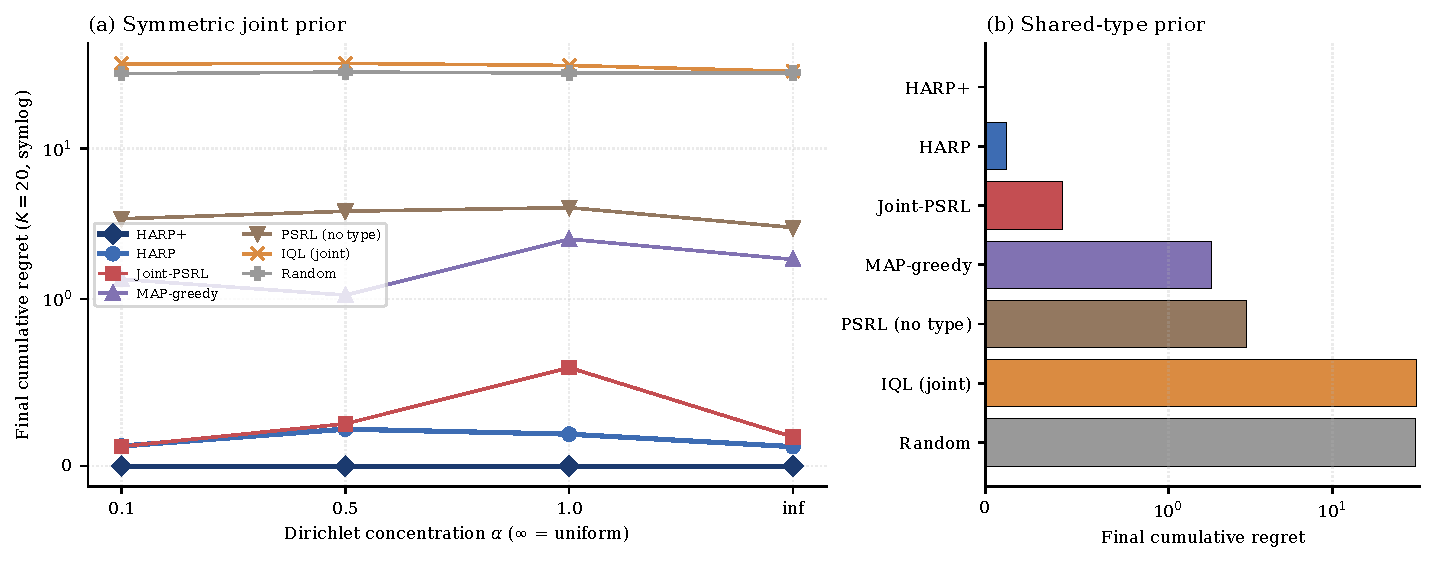
\includegraphics[width=\columnwidth]{figs/fig_e1_3_pf_isolation.pdf}
  \caption{C4 prior swap on HP-SPGG ($n{=}3$, $|\Theta|{=}4$, $|\Theta|^n{=}64$ joint profiles, $K{=}20$, $10$ common environment seeds, $\beta{=}0.25$, analytic calibration). \emph{Left:} symmetric Dirichlet sweep on the $64$-simplex; each seed draws $p\!\sim\!\mathrm{Dir}(\alpha\mathbf{1}_{64})$ and HARP inherits the induced marginals while the explicit joint baseline uses $p$. \emph{Right:} a shared-type prior, uniform over the four same-type profiles, leaves marginals uniform while maximally coupling them. The HARP family stays within $0.6$ cumulative regret on every retained cell.}
  \label{fig:e1-3-pf}
\end{figure}

\paragraph{True shared-type DGP.}
The dual intervention makes the data-generating process itself fully coupled. Joint-PSRL-Aware's same-type prior is then well-specified while HARP's independent marginal prior is misspecified relative to the truth.

\paragraph{Setup.} At the start of each episode a single type $t \sim \mathrm{Uniform}(\Theta)$ is drawn and assigned to every agent, so $\theta_i^\star = t$ for all $i$. HARP (uniform marginals, factored representation), Joint-PSRL-Uniform (uniform Dirichlet over the $|\Theta_i|^n$ joint profiles), and Joint-PSRL-Aware (strict prior on the $m$ same-type profiles) share the same likelihood model, backward-induction joint-action planner, and common environment seeds. We sweep $n\!\in\!\{3,4,5\}$ and $K\!\in\!\{50,100\}$ on one analytic kernel and four live LLM backbones (DeepSeek-V3.2, GPT-5.4-nano, Kimi-K2.6, Llama-4-Maverick) with $10$ common environment seeds per cell and $\beta{=}0.25$. Posterior storage at $n{=}5$ is $20$ parameters for HARP, $1024$ for Joint-PSRL-Uniform, and $4$ for Joint-PSRL-Aware.

\begin{table*}[h]
\centering\small
\caption{True shared-type DGP robustness on HP-SPGG across one analytic kernel and four live LLM backbones ($m{=}|\Theta_i|{=}4$, $K{=}100$, $10$ common environment seeds, $\beta{=}0.25$). True types are drawn from the $m$ same-type joint profiles, so Joint-PSRL-Aware's strict prior is well-specified and HARP's factored prior is mis-specified relative to the coupled truth. HARP remains within $1.5\times$ of Aware on $14$ of $15$ cells (Kimi-K2.6 $n{=}4$ at $1.52\times$); the GPT-5.4-nano $n{=}4$ cell where Aware reaches $0$ is marked with a dash. HARP is lower-regret than Aware on $9$ of $15$ cells.}
\label{tab:true-shared-dgp}
\setlength{\tabcolsep}{8pt}
\begin{tabular}{@{}lcccc@{}}
\toprule
Substrate & $n$ & HARP & J-PSRL-A & HARP $/$ Aware \\
\midrule
analytic kernel       & 3 & 0.28 & 0.22 & 1.29$\times$ \\
                      & 4 & 0.00 & 0.32 & 0.00$\times$ \\
                      & 5 & 0.31 & 0.39 & 0.79$\times$ \\
\midrule
DeepSeek-V3.2         & 3 & 1.79 & 1.23 & 1.46$\times$ \\
                      & 4 & 1.31 & 1.84 & 0.71$\times$ \\
                      & 5 & 2.11 & 2.61 & 0.81$\times$ \\
\midrule
GPT-5.4-nano          & 3 & 0.64 & 0.74 & 0.86$\times$ \\
                      & 4 & 0.22 & 0.00 & --           \\
                      & 5 & 1.64 & 2.36 & 0.69$\times$ \\
\midrule
Kimi-K2.6             & 3 & 1.14 & 0.86 & 1.32$\times$ \\
                      & 4 & 1.49 & 0.99 & \textbf{1.52$\times$} \\
                      & 5 & 1.15 & 1.47 & 0.78$\times$ \\
\midrule
Llama-4-Maverick      & 3 & 1.72 & 1.49 & 1.16$\times$ \\
                      & 4 & 1.59 & 1.07 & 1.49$\times$ \\
                      & 5 & 1.76 & 1.38 & 1.27$\times$ \\
\bottomrule
\end{tabular}
\end{table*}

\paragraph{Reading.} Under the coupled DGP, HARP remains within $1.52\times$ of the correctly supported Joint-PSRL-Aware on every reported cell and is lower-regret on $9$ of $15$. This is robustness under PF violation, not exact decoupling: C1's equality claim remains restricted to TI/RL/PF, while Table~\ref{tab:storage-comparison} provides the representation-only comparison under the well-specified iid DGP.


\subsection{RQ3: Component Attribution}
\label{app:rate-burnin}

This subsection certifies C2, C3, and C6, attributing the gains to their components. C2 and C3 first: HARP exhibits the $\tilde O(\sqrt K)$ plateau-versus-linear separation from type-agnostic sampling, and HARP\textsuperscript{+}'s type-discrimination bonus shortens burn-in on slowly concentrating backbones without degrading the others.

\begin{figure*}[t]
  \centering
  \subfloat[C2: per-episode trajectory.\label{fig:e5}]{
\includegraphics[width=\textwidth]{figs/fig_e5_cumulative_regret_trajectories_v3.pdf}}\hfill
  \subfloat[C3: concentration speed and bonus benefit.\label{fig:e1}]{
\includegraphics[width=0.48\textwidth]{figs/fig_e1_posterior_concentration_v3.pdf}}
  \caption{Rate and burn-in evidence. (a) HARP and HARP\textsuperscript{+} plateau at $<0.05$ regret per episode within $K{\approx}5$ on four HP-SPGG backbones, while PSRL-NoType grows linearly and reaches an $11$--$30\times$ cumulative gap at $K{=}20$. (b) Vanilla-HARP concentration time $K_{\mathrm{conc}}^{0.9}$ predicts the benefit of the $\beta=0.25$ discrimination bonus across the four backbones.}
  \label{fig:e2-e5}
\end{figure*}



\subsubsection{Update Value and Rate (C2)}

\paragraph{HP-SPGG rate and concentration.}
Figure~\ref{fig:e2-e5}(a) realizes the rate separation of Theorem~\ref{thm:rate-separation}; panel (b) recovers the three regimes of Theorem~\ref{thm:pact-plus-app}. Concentration times are DeepSeek $4.4$, GPT $6.6$, Kimi $12.0$, and Llama $14.0$ episodes out of $K=20$. The privileged analytic-kernel cross-check in Figure~\ref{fig:app-e2-native} places HARP\textsuperscript{+} within $0.05$ regret of the noise-free reference on every backbone.

\begin{figure}[t]
  \centering
  
\includegraphics[width=\columnwidth]{figs/E2_native_vs_llm_baselines_main.pdf}
  \caption{C2 analytic-kernel cross-check: HARP\textsuperscript{+} on HP-SPGG c19 remains within $0.05$ regret of the privileged analytic-kernel reference across all four backbones.}
  \label{fig:app-e2-native}
\end{figure}
\paragraph{Iterated Concordia-derived diagnostic.}
The native compact Concordia evaluation is one-shot. We therefore construct a fixed-persona $K{=}20$ diagnostic from six configurations selected on seeds $0$--$4$ and report on disjoint seeds $1000$--$1004$. It retains the upstream sampler, exact payoff, and finite menu, imposes PF, and uses the same Gaussian update after reward normalization. It is Concordia-derived rather than native, and exact-payoff replay is backbone-invariant. Figure~\ref{fig:iterated-concordia} and Table~\ref{tab:iterated-concordia} show HARP, HARP\textsuperscript{+}, and Joint-PSRL flattening after identification, while PSRL-NoType continues accumulating regret. HARP\textsuperscript{+} reaches $0.352\pm0.035$ cumulative and $0.0020\pm0.0017$ late regret, versus $1.361\pm0.172$ and $0.0764\pm0.0139$ for PSRL-NoType; HARP and Joint-PSRL remain within paired uncertainty.

\begin{table}[t]
\centering\small
\caption{Iterated Concordia-derived aggregate at $K{=}20$. Late is mean instant regret over episodes $11$--$20$.}
\label{tab:iterated-concordia}
\begin{tabular}{lcc}
\toprule
Method & Cumulative regret & Late regret \\
\midrule
HARP & $0.312\pm0.026$ & $0.0041\pm0.0012$ \\
HARP\textsuperscript{+} & $0.352\pm0.035$ & $0.0020\pm0.0017$ \\
Joint-PSRL & $0.329\pm0.030$ & $0.0049\pm0.0012$ \\
PSRL-NoType & $1.361\pm0.172$ & $0.0764\pm0.0139$ \\
\bottomrule
\end{tabular}
\end{table}

\subsubsection{Discrimination Bonus (C3)}

\paragraph{Bonus scaling and frozen coefficient.}
Figure~\ref{fig:n-scaling} shows the bonus under type- and agent-space growth. Figure~\ref{fig:beta-sweep} selects $\beta=0.25$ as the smallest value in the no-degradation interval, cutting slowest-backbone regret from $0.97$ to $0.31$. Table~\ref{tab:bonus-ablation} holds likelihood, posterior, sampling, and policy interface fixed and changes only $\beta$ on downstream substrates.

\begin{figure}[t]
  \centering
  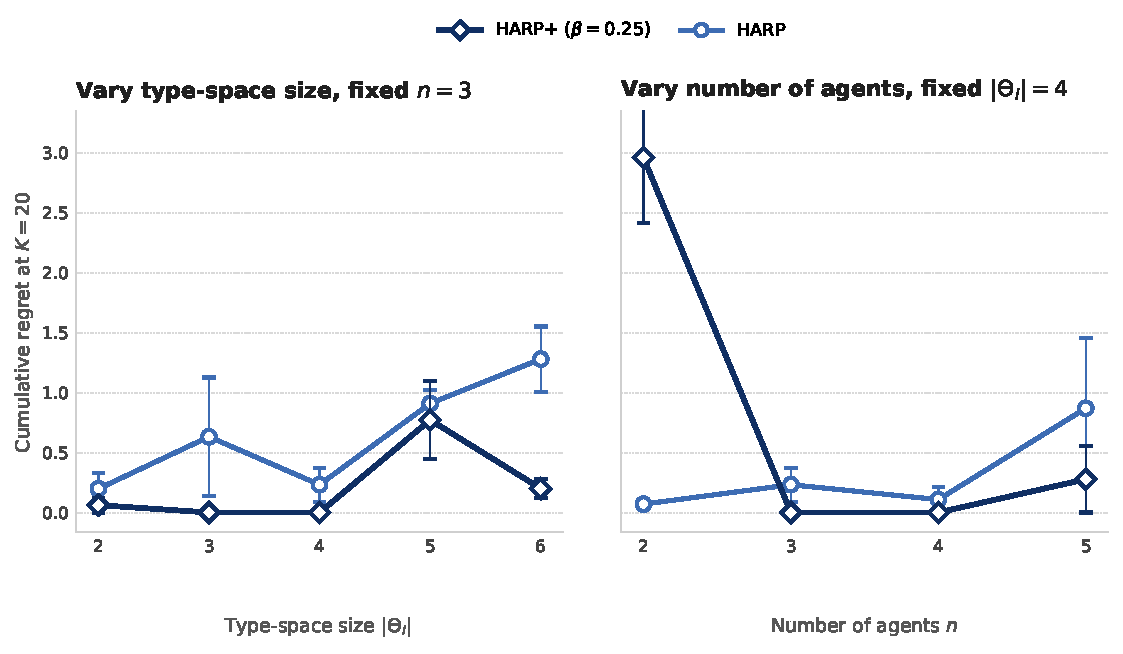
\includegraphics[width=\columnwidth]{figs/fig_scaling_hidden_complexity_v5.pdf}
  \caption{C3 scaling of HARP and HARP\textsuperscript{+} on HP-SPGG. Left varies $|\Theta_i|$ at $n=3$; right varies $n$ at $|\Theta_i|=4$. Curves report $K=20$ cumulative regret over $10$ seeds on Llama-4-Maverick with $\beta=0.25$.}
  \label{fig:n-scaling}
\end{figure}

\begin{figure}[t]
  \centering
  
\includegraphics[width=0.8\columnwidth]{figs/fig10_beta_sweep_v3.pdf}
  \caption{C3 HP-SPGG $\beta$-sweep at $K=20$. The frozen value $\beta=0.25$ is the smallest point in the no-degradation interval $[0.25,0.75]$; it leaves three saturated backbones unchanged and reduces Llama-Maverick regret from $0.97$ to $0.31$.}
  \label{fig:beta-sweep}
\end{figure}

\begin{table}[t]
\centering\small
\caption{C3 direct type-discrimination bonus ablation. HARP and HARP\textsuperscript{+} share likelihood, posterior, sampling, and solver; only $\beta$ changes. Concordia is single-shot, so the multi-step concentration mechanism is inactive. MaaSSim rows are E-F fixed-state replay with frozen $\beta{=}0.25$; the bonus changes $4$ of $406$ assignments and the paired gap covers zero. Historical SOTOPIA rows are descriptive because that tracker remained at its prior.}
\label{tab:bonus-ablation}
\setlength{\tabcolsep}{6pt}
\begin{tabular}{@{}lccc@{}}
\toprule
 & HARP & HARP\textsuperscript{+} & $\Delta$ \\
\midrule
\multicolumn{4}{l}{\emph{Concordia (single-shot)}} \\
Pub Coordination               & $1.264$ & $1.264$ & $+0.000$ \\
Haggling (single-item)         & $3.661$ & $3.661$ & $+0.000$ \\
Haggling (multi-item)          & $5.429$ & $5.429$ & $+0.000$ \\
\midrule
\multicolumn{4}{l}{\emph{MaaSSim replay (E-F, $10$ seeds, utility)}} \\
Dispatch utility               & $27.61$ & $27.36$ & $-0.25$ \\
\midrule
\multicolumn{4}{l}{\emph{SOTOPIA-Hard ($6$-turn, $n{=}70$/cell)}} \\
DeepSeek-V3.2                  & $3.242$ & $3.248$ & $+0.006$ \\
GPT-5.4-nano                   & $2.873$ & $2.981$ & $+0.107$ \\
Kimi-K2.6                      & $2.789$ & $2.807$ & $+0.018$ \\
Llama-Maverick                 & $3.308$ & $3.308$ & $+0.000$ \\
\emph{Mean (SOTOPIA-Hard)}     & $3.053$ & $3.086$ & $+0.033$ \\
\bottomrule
\end{tabular}
\end{table}

Only HP-SPGG supports interpreting the bonus as accelerated concentration. The downstream table establishes numerical activity and scope: no effect in one-shot Concordia and a small descriptive SOTOPIA difference that is not update evidence.

\subsubsection{Mechanism: Identity and Dispatch (C6)}
\label{app:mechanism}
\label{app:ablations}
\label{app:decent-extended}

This subsection certifies C6: gains require both correctly identity-attached posterior mass and a centralized dispatcher that converts one joint belief draw into a coordinated action.

\paragraph{Component ablation (E-G).} Analytic HP-SPGG with $10$ common seeds, $K{=}20$, $\beta{=}0.25$, and a shared profile, prior, tensor, and oracle per seed. The \emph{minus identity} variant keeps correct closed-form updates and attaches posterior rows through a fixed seed-derived derangement at planning time. The \emph{minus dispatch} variant gives every actor the same public-history posterior with independent profile sampling and own-utility best response. Endpoint regrets are full $0.015\pm0.007$, minus bonus $0.016\pm0.007$, minus update $0.675\pm0.114$, minus identity $0.700\pm0.368$ (seeds $3$, $4$, $7$, $9$ carry the whole effect), and minus dispatch $6.324\pm0.439$. Paired $95\%$ CIs against full are $[-0.002,0.003]$ for minus bonus, $[0.41,0.92]$ for minus update, $[-0.14,1.51]$ for minus identity, and $[5.31,7.31]$ for minus dispatch. The minus-dispatch variant bundles two changes, independent profile sampling and a switch from joint welfare to own-utility best response, so its endpoint bounds the value of joint commitment from above rather than isolating it. The mode comparison of Figure~\ref{fig:decentralized-price} separates the two. All four modes there select on own or focal payoff, so the objective is held approximately fixed while commitment varies, and the two centralized modes still differ from the two decentralized ones by a $3$--$4\times$ cumulative-regret slope, with the same ordering on the welfare sum over all five players. Joint commitment therefore carries the bulk of the effect and the objective switch the remainder.

\begin{figure*}[t]
  \centering
  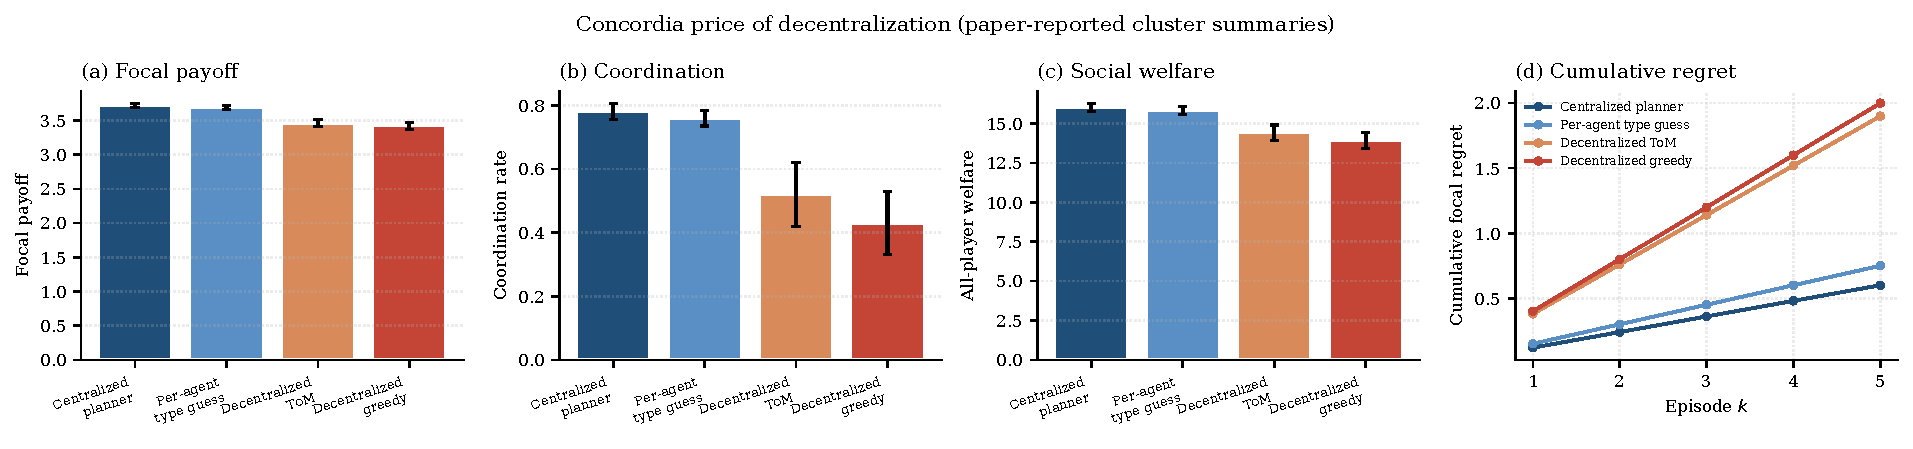
\includegraphics[width=\textwidth]{figs/fig12_decentralized_price.pdf}
  \caption{Price of decentralization on Concordia \texttt{london\_mini} Pub Coordination ($5$ players, $2$ focal, $5$ scenes per cell). Centralized (planner LLM, per-agent type-guess) vs.\ decentralized (ToM-prompted, greedy), same LLM. \emph{(a)} Focal payoff. \emph{(b)} Coordination. \emph{(c)} Social welfare. \emph{(d)} Cumulative regret over $K{=}5$ scenes (bands: SE over backbones). Centralized modes cluster near \texttt{oracle\_joint}; decentralized modes: $-0.2$--$0.3$ payoff, $-0.2$--$0.4$ coordination, $-1$--$2$ welfare units, $3$--$4\times$ cumulative regret.}
  \label{fig:decentralized-price}
\end{figure*}

HARP\textsuperscript{+} rests on two complementary components, \emph{centralized dispatch} and the \emph{closed-form Bayesian tracker}. This part isolates dispatch. The historical SOTOPIA-Hard comparison above is descriptive because its tracker did not update; the corrected recurrent evidence is reported separately in Section~\ref{app:sotopia-corrected}.

We compare four dispatch modes sharing the same LLM on \texttt{london\_mini} Pub Coordination ($5$ players, $2$ focal, $5$ seeds per backbone), two centralized (planner LLM emitting the joint action, per-agent type-guess producing $n$ independent posteriors) and two decentralized (greedy, ToM-prompted). Within-cluster differences isolate planning-vs-belief and cluster differences isolate dispatch, with \texttt{oracle\_joint} as the ceiling and full mode definitions below.

Two clusters emerge on every backbone and every metric (Figure~\ref{fig:decentralized-price}). Within-cluster planning-vs-belief differences stay below $0.05$ on focal payoff, while the centralized-to-decentralized gap produces a $3$--$4\times$ cumulative-regret slope difference. Joint exploration requires one planner to commit all agents to the same sampled profile; independently prompted agents miscoordinate on the states the posterior is meant to resolve. Corrected recurrent tracker controls are reported in Section~\ref{app:sotopia-corrected}, so the dispatch and belief-identity mechanisms are documented separately rather than inferred from the deleted static-tracker ablation.

The remainder of this part gives the full per-backbone breakdown, the per-metric definitions, and the additional analysis.

\paragraph{Per-mode definitions.} The four dispatch modes evaluated are:
\begin{itemize}\itemsep -1pt \topsep -2pt
  \item \emph{Centralized planner LLM}, one LLM call sees the full relationship-statement matrix for all $5$ players and outputs a joint posterior over every player's favorite pub, and argmax yields the joint action.
  \item \emph{Per-agent type-guess LLM}, $n$ independent LLM calls, each restricted to a single player's own social context, each outputting a posterior over that one player's favorite pub.
  \item \emph{Decentralized LLM (ToM)}, $n$ independent LLM calls, each agent is prompted to balance own preference with theory-of-mind reasoning and pick \emph{one} pub.
  \item \emph{Decentralized LLM (greedy)}, $n$ independent LLM calls, each agent picks the pub maximizing its own expected enjoyment with no partner inference.
\end{itemize}

\paragraph{Within-cluster ordering.} The relative ordering inside the centralized cluster is informative for the underlying mechanism. On GPT-5.4-nano and Llama-4-Maverick the global-view planner edges the per-agent type-guess variant ($+0.10$ payoff), as expected if joint observation is the load-bearing factor. On DeepSeek-V3.2 and Kimi-K2.6 the order flips by $+0.05$. The per-agent variant slightly beats the planner because the planner occasionally splits the $2$ focal players across the $2$ pubs (coordination $0.80$/$0.90$ vs.\ $1.00$ for the per-agent variant), while the per-agent variant defaults to the more popular pub. The structural conclusion is the same in both directions. The lift comes from the \emph{probabilistic-reasoning prompt over a posterior on the partner's persona}, irrespective of whether that posterior is computed once jointly or $n$ times in parallel.

\paragraph{Welfare-over-all-players check.} Panel (c) of Figure~\ref{fig:decentralized-price} reports the welfare sum over all $5$ players (not just focal), matching the theoretical objective $W = \sum_i r_i$ used in Section~\ref{sec:algorithm}. The centralized cluster still leads the decentralized cluster by $1$--$2$ units on every backbone, so the main-text gap is not produced by NPC-side noise aligned with the focal players.

\paragraph{Cumulative compounding.} Panel (d) shows the per-episode gap compounds. By the end of $5$ episodes, decentralized modes accumulate $1.9$--$2.0$ units of focal regret while centralized modes stay at $0.6$--$0.75$, the $3$--$4\times$ slope ratio reported in the main text. This linear-in-$K$ accumulation is the price-of-decentralization analogue of the HP-SPGG cumulative-regret divergence in Figure~\ref{fig:hp-spgg-cross-model}, but within a single LLM backbone. The slope difference is structural to the dispatch mode rather than to the model's individual social-inference quality.

\paragraph{MaaSSim fixed-state mechanism replay.}
\label{app:maassim}

This part expands Section~\ref{sec:maassim} only to certify C6: it isolates posterior concentration and driver-identity attachment on common saved decision states, then reports a directional single-backbone dispatch suite.

\paragraph{Substrate and replay protocol.}
Runs use the Nootdorp road-network scenario with $40$ passengers, $8$ vehicles, and $120$-second dispatch batches. Each driver carries a hidden operational rule sampled from \{\texttt{avoid\_long}, \texttt{zone\_loyal}, \texttt{home\_pull}, \texttt{surge\_sensitive}\}, applied inside the simulator as accept/reject behavior, and the coordinator observes only which offers each driver accepts or rejects. Evaluation uses fixed-state replay. Queue snapshots and realized persona maps are saved from closed-loop runs, and every method is evaluated on the identical states, which removes the state-distribution feedback that otherwise confounds closed-loop dispatch comparisons. Realized utility combines a serve value of $3.0$ per served ride, a pickup-wait cost of $0.01$ per second, a driver-reject penalty of $2.0$ ($5.0$ under stress), and a passenger-reject penalty of $0.5$.

\paragraph{Persona-mechanism ablation.}
Table~\ref{tab:maassim-mechanism} and Figure~\ref{fig:maassim-mechanism} report the mechanism ablation over $10$ seeds. All HARP variants share one assignment objective and the same states, and only the driver-belief source changes, so the comparison isolates the value of the learned posterior itself. The learned posterior improves realized utility over a uniform prior by $+16.50$ ($27.61$ vs.\ $11.11$), closing $59.3\%$ of the prior-to-oracle gap. The shuffled control, which attaches each learned posterior to the wrong driver, collapses to $6.87$, below even the uniform prior, although its marginal rule accuracy ($0.521$) is nominally above chance. Recovered beliefs are therefore useful only when attached to the correct driver identity. The gain is not free. HARP accepts $16.25$ seconds of extra pickup wait per snapshot to reduce driver rejections and serve more passengers, so this table supports a persona-mechanism claim rather than a wait-minimization claim. Decomposing the tracker's per-observation belief gain by event type over the same posterior trajectories, rejections contribute a mean marginal rule-accuracy gain of $0.038$ per event ($n{=}279$) against $0.022$ for accepts ($n{=}388$), a $\approx\!1.7\times$ ratio with the same direction on exact-type mass ($0.031$ vs.\ $0.020$). This asymmetry is expected because all four hidden rules act as rejection triggers, so rejections are the type-revealing events. Figure~\ref{fig:maassim-concentration} traces the concentration itself: over the per-driver observation sequence, marginal rule accuracy rises from chance $0.53$ to $0.73$ and exact-type posterior mass from the $1/16$ uniform prior to $0.26$ within $8$ observations, consistently across seeds.

\begin{figure}[t]
  \centering
  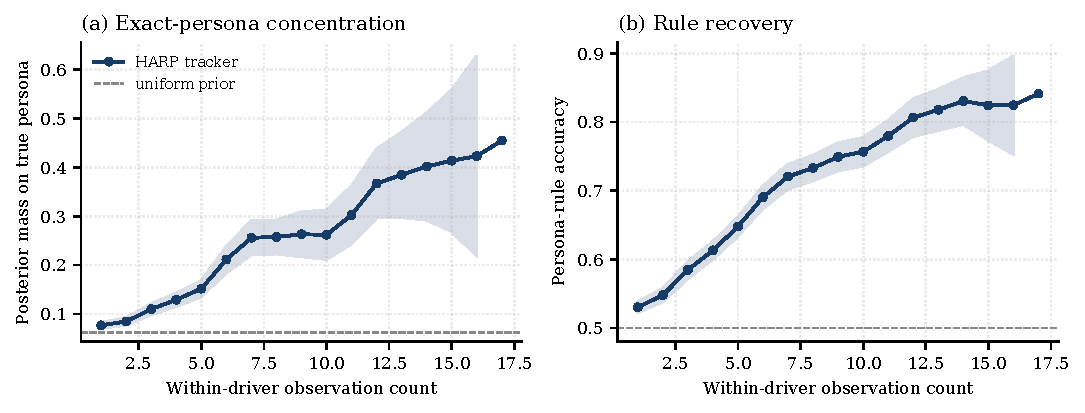
\includegraphics[width=\columnwidth]{figs/fig_maassim_concentration_v1.pdf}
  \caption{HARP driver-belief concentration on MaaSSim ($10$ seeds, thin lines are per-seed means, bands are SEM over (seed, driver) pairs). From accept/reject observations alone, marginal rule accuracy and exact-type posterior mass rise well above their chance references within a handful of observations of each driver.}
  \label{fig:maassim-concentration}
\end{figure}

\begin{table}[t]
\centering
\scriptsize
\setlength{\tabcolsep}{2.5pt}
\begin{tabular}{llrrrr}
\toprule
Variant & Belief source & Utility & Rejects & Accept & Rule acc. \\
\midrule
Nearest & none & $11.03$ & $26.0$ & $0.634$ & --- \\
Random & none & $-33.94$ & $30.6$ & $0.563$ & --- \\
HARP-prior & uniform & $11.11$ & $25.1$ & $0.635$ & $0.500$ \\
HARP-shuffled & wrong driver & $6.87$ & $26.5$ & $0.609$ & $0.521$ \\
HARP & learned & $\mathbf{27.61}$ & $\mathbf{18.5}$ & $\mathbf{0.740}$ & $0.720$ \\
Oracle & true persona & $38.92$ & $13.2$ & $0.822$ & $1.000$ \\
\bottomrule
\end{tabular}
\caption{MaaSSim persona-mechanism replay ($10$ seeds, fixed queue snapshots and persona maps, shared assignment objective). Utility is the realized dispatch utility defined above (seed-level SEM $9.6$--$11.7$); Rejects is mean driver rejects; Accept is the driver acceptance rate; Rule acc.\ is the marginal accuracy of the belief on the true driver rule.}
\label{tab:maassim-mechanism}
\end{table}

HARP trades approximately $9$ seconds of additional mean pickup wait for $6.6$ fewer driver rejections than the uniform-prior variant; at comparable wait, the shuffled-identity control produces more rejections, so identity attachment rather than sharper marginals alone drives the gain.

\begin{figure}[t]
  \centering
  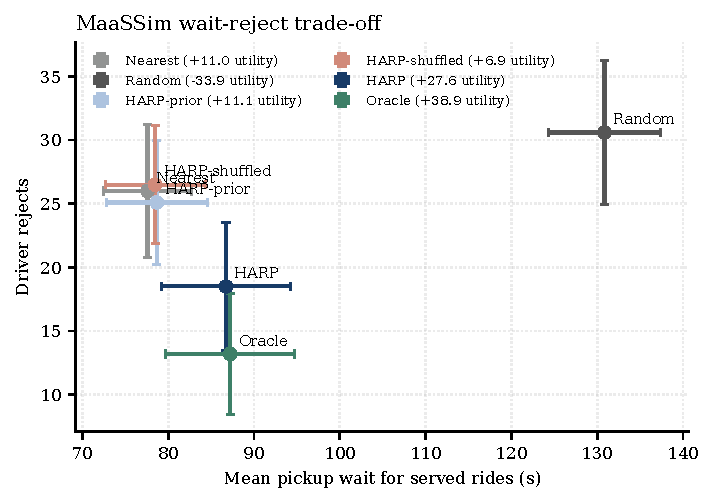
\includegraphics[width=0.85\columnwidth]{figs/fig_maassim_wait_reject_tradeoff_v1.pdf}
  \caption{Operating points of the mechanism-replay variants ($10$ seeds, SEM bars on both axes). HARP trades pickup wait for fewer driver rejects, moving from the uniform-prior operating point toward the oracle (dashed arrow), while the shuffled control stays at the heuristic wait level with more rejects. This is why Table~\ref{tab:maassim-mechanism} supports a persona-mechanism claim rather than a wait-minimization claim.}
  \label{fig:maassim-tradeoff}
\end{figure}

\begin{figure}[t]
  \centering
  
\includegraphics[width=\columnwidth]{figs/fig_maassim_pact_persona_mechanism.pdf}
  \caption{MaaSSim persona-mechanism replay. All variants share the same fixed queue snapshots, persona maps, and assignment objective, and only the driver-belief source changes. The learned posterior (HARP) closes $59.3\%$ of the prior-to-oracle utility gap, while the shuffled-posterior control falls below the uniform prior, showing that correct driver-identity attachment is necessary for the gain.}
  \label{fig:maassim-mechanism}
\end{figure}

\paragraph{LLM dispatch replay.}
The LLM experiments use \texttt{gpt-5.4-mini} (pinned snapshot \texttt{20260317}) over $5$ seeds with the first $20$ active snapshots per seed. Each LLM policy receives a legal one-to-one assignment menu plus method-specific context and returns JSON containing an \texttt{assignment\_id}; across all reported LLM methods the parse rate is $1.000$ with no repairs and no fallbacks, so the action interface itself is not a confound. The prompt baselines mirror the main-text families, namely \texttt{llm\_belief}, LLM-PSRL, A-ToM, and ECON-BNE. HARP is a score-assisted hybrid that receives HARP assignment scores in context, not a pure prompt method. Table~\ref{tab:maassim-scenarios} reports a controlled conflict-strength sweep. All cells use driver-reject penalty $5.0$ and common snapshots. For each candidate offer, $\lambda\in\{0,0.5,1\}$ interpolates travel time and fare between the retained reject-stress offer and the full persona-risky conflict transformation; policies are rerun at every level rather than interpolating outcomes. The hybrid's advantage over the best pure prompt baseline grows monotonically from $+4.60$ to $+31.75$ and $+39.69$. At $\lambda=1$, every pure prompt baseline has negative utility (best $-30.90$) while the hybrid remains positive at $8.79$ against an oracle at $22.44$. The full-conflict endpoint is a designed stress test, not an estimate of normal operations.

\begin{table}[t]
\centering
\scriptsize
\setlength{\tabcolsep}{3pt}
\begin{tabular}{@{}lrlrr@{}}
\toprule
Scenario & HARP & Best prompt & Gap & Oracle \\
\midrule
Reject ($\lambda=0$) & $18.37$ & PSRL: $13.77$ & $+4.60$ & $36.44$ \\
Mid ($\lambda=.5$) & $8.96$ & belief: $-22.80$ & $+31.75$ & $30.70$ \\
Full ($\lambda=1$) & $\mathbf{8.79}$ & belief: $-30.90$ & $+39.69$ & $22.44$ \\
\bottomrule
\end{tabular}
\caption{MaaSSim LLM dispatch conflict-strength sweep (\texttt{gpt-5.4-mini}, $5$ seeds $\times$ $20$ snapshots, driver-reject penalty $5.0$, parse rate $1.000$). Best prompt is the strongest pure prompt baseline per level; Gap is HARP minus best prompt. Outcomes are measured reruns at $\lambda\in\{0,0.5,1\}$, not interpolated results.}
\label{tab:maassim-scenarios}
\end{table}

\paragraph{Full-conflict episode dynamics.}
Figure~\ref{fig:maassim-conflict-dynamics} traces single $\lambda{=}1$ replay episodes for the hybrid and the three strongest prompt baselines on a common seed, complementing the aggregate sweep of Table~\ref{tab:maassim-scenarios} with per-episode evidence. The prompt baselines repeatedly issue persona-risky low-wait assignments, accumulate $14$ to $15$ driver rejects, and end with negative utility, while the hybrid holds rejects to $2$ and serves $19$ requests. The aggregate collapse is therefore visible within individual episodes rather than an artefact of averaging.

\begin{figure*}[t]
  \centering
  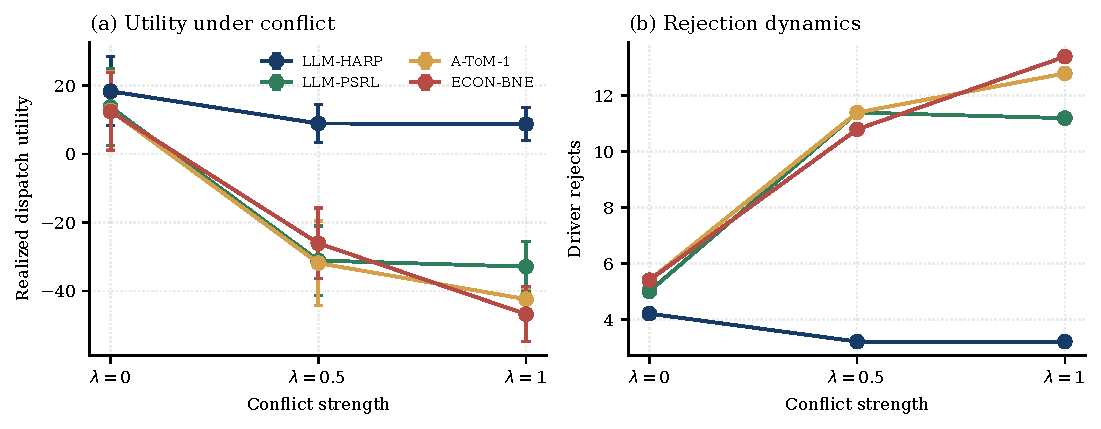
\includegraphics[width=0.98\textwidth]{figs/fig_maassim_conflict_dynamics_v4.pdf}
  \caption{Single-episode conflict-offer replay dynamics ($\lambda{=}1$) for HARP, LLM-PSRL, A-ToM-1, and ECON-BNE on a common seed: vehicle and request traces with cumulative utility, served requests, and driver rejects per decision step.}
  \label{fig:maassim-conflict-dynamics}
\end{figure*}

\paragraph{Unit validation for the main-text regret panel.}
Figure~\ref{fig:maassim-main}(b) reports oracle regret divided by the common reject penalty $5.0$, with vertical bars propagating the retained seed-level oracle and policy utility SEMs as $\sqrt{\mathrm{SEM}_{\rm oracle}^2+\mathrm{SEM}_{\rm policy}^2}/5$; the paired seed-level covariance was not retained. Figure~\ref{fig:maassim-unit-validation} validates that unit against observable behavior by plotting it against excess driver rejects for all method-scenario pairs. Points track the identity line, and conflict-offer points sit slightly above it because failed episodes also forfeit served rides.

\begin{figure}[t]
  \centering
  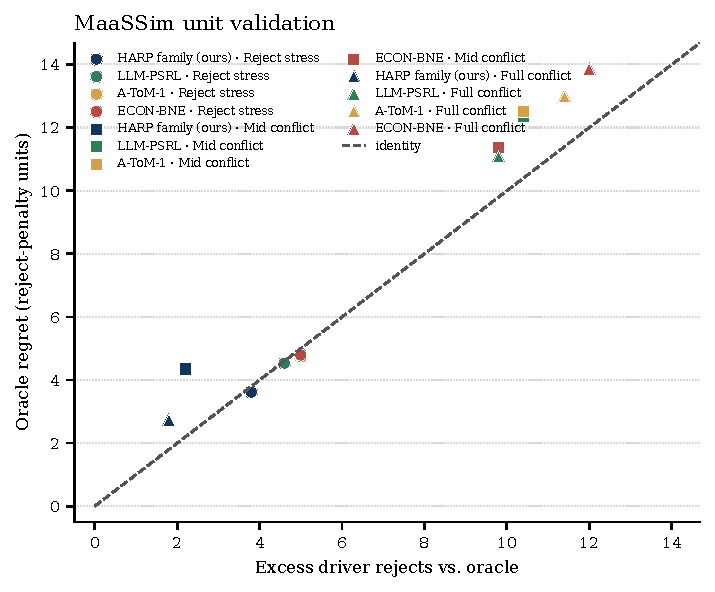
\includegraphics[width=0.9\columnwidth]{figs/fig_maassim_unit_validation_v3.pdf}
  \caption{Unit validation for the main-text regret panel. Oracle regret in reject-penalty units against excess driver rejects relative to the oracle, for six methods across three measured replay scenarios ($5$ seeds).}
  \label{fig:maassim-unit-validation}
\end{figure}

\paragraph{Scope and limitations.}
Hidden types are synthetic rules rather than learned human driver preferences, results cover one road network and one LLM backbone, and the LLM tables aggregate five seeds without retained per-seed outcomes, so no paired significance test is possible. Passenger-side inference is weak because most riders are observed once (rule accuracy $\approx 0.53$ against a $0.5$ chance level), and the retained persona libraries are too small for the HARP\textsuperscript{+} exploration bonus to alter assignments, so no claim in this subsection relies on HARP\textsuperscript{+} or on passenger inference.


\subsection{Oracle Constructions (Shared Infrastructure)}
\label{app:oracles}
\label{app:oracle-construction}

This subsection supports C1--C6 by certifying what each oracle reference knows and optimizes; it is shared evaluation infrastructure, not an additional empirical claim.

\begin{figure}[t]
  \centering
  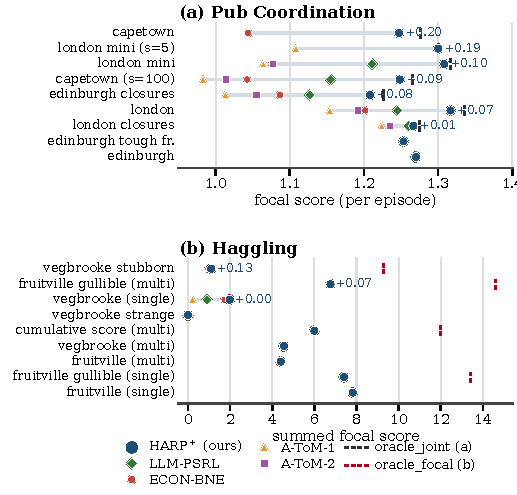
\includegraphics[width=\columnwidth]{figs/fig2_concordia_strip_v11c.pdf}
  \caption{Full Concordia comparison across all $18$ configurations. Pub Coordination uses \texttt{oracle\_joint}; Haggling uses the exact full-information focal ceiling \texttt{oracle\_focal}. Rows are sorted by HARP\textsuperscript{+}'s margin over the strongest baseline.}
  \label{fig:concordia-full}
\end{figure}

The three LLM benchmarks differ along two axes: whether payoff is closed-form and whether the action space is finite and enumerable. In every case the privileged signal is the true opponent type; the payoff or judge is part of the environment and is available to all methods.

\paragraph{HP-SPGG.}
The oracle exhaustively enumerates the finite joint contribution grid and applies a deterministic argmax to the same pinned tensor used by every method. It is therefore an exact pointwise reference for the regret calculation.

\paragraph{Concordia.}
The compact Pub and Haggling evaluators expose a finite menu and analytic \texttt{payoff\_for\_case}. \texttt{oracle\_joint} exactly maximizes joint welfare. Because Haggling price is a transfer, that objective is not a focal ceiling; \texttt{oracle\_focal} reruns the same exhaustive search on focal payoff and is never exceeded. Figure~\ref{fig:haggling-pareto} displays the objective trade-off.

\begin{figure}[t]
  \centering
  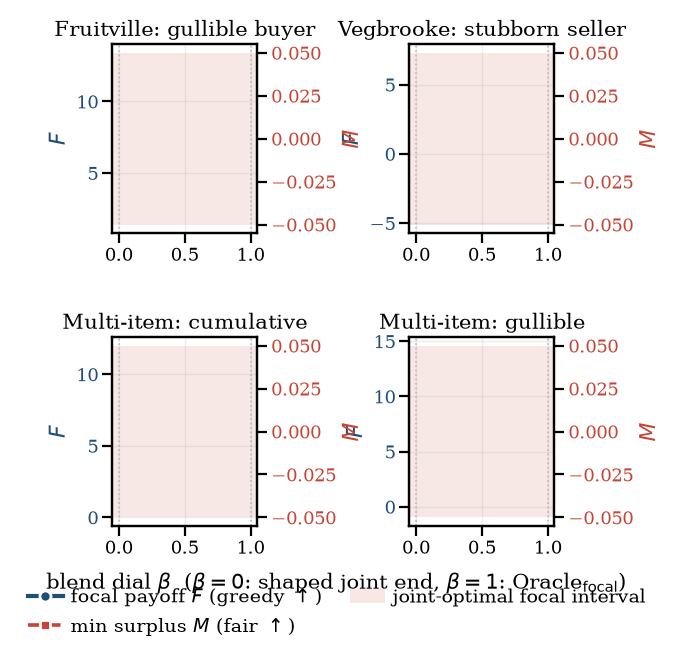
\includegraphics[width=\columnwidth]{figs/fig11_haggling_pareto.png}
  \caption{Focal-vs-joint Haggling frontier. $\beta_{\mathrm{obj}}=0$ is \texttt{oracle\_joint} (J); $\beta_{\mathrm{obj}}=1$ is \texttt{oracle\_focal} (F). Increasing focal payoff can reduce minimum participant surplus, explaining why a focal policy may exceed the joint oracle's focal score without violating an upper bound.}
  \label{fig:haggling-pareto}
\end{figure}

\paragraph{SOTOPIA-Hard.}
Open-ended utterances and a seven-dimensional LLM judge preclude exact enumeration. \texttt{oracle\_belief} supplies the one-hot opponent persona but retains single-shot generation; it is not a strict upper bound. \texttt{oracle\_policy} draws five independent episodes and retains the one with highest mean judge score. The second block of Table~\ref{tab:sotopia-aggregate} reports both rows. Their gap measures action-search and judge-variance headroom rather than persona-information value alone.

\begin{table*}[t]
\centering\small
\caption{Oracle construction across the three LLM benchmarks.}
\label{tab:oracle-summary}
\setlength{\tabcolsep}{6pt}
\begin{tabular}{llll}
\toprule
Benchmark & Payoff form & Action space & Oracle type \\
\midrule
HP-SPGG & analytic/pinned tensor & finite, $125$ joint profiles & strict exhaustive argmax \\
Concordia & analytic, closed-form & finite menu & strict joint/focal argmax \\
SOTOPIA-Hard & 7-dimensional LLM judge & open-ended utterance & belief-only $+$ best-of-$K$ critic \\
\bottomrule
\end{tabular}
\end{table*}


\section{Theoretical Supplement}
\label{app:theory}

\subsection{Overview and Claim-to-Theorem Map}
\label{app:theory-overview}

This appendix gives the formal setting, assumptions, and proofs supporting every theoretical statement in Section~\ref{sec:pact-vanilla}--\ref{sec:pact-plus-algo}. Table~\ref{tab:theorem-map} keys each main-text claim to the formal statement and proof location. The subsections follow the order of the claims in the table. The remainder of this appendix is organized as: formal setting (Section~\ref{sec:setting-app}), posterior decoupling (Section~\ref{app:decoupling-proof}), necessity of TI and RL (Section~\ref{app:necessity}), regret bound (Section~\ref{app:regret-bound}), scorer misspecification (Section~\ref{app:misspec}), approximate decoupling (Section~\ref{app:approx-decoupling}), unbounded coupling and the RL threshold (Section~\ref{app:unbounded-coupling}), rate separation (Section~\ref{app:rate-separation}), HARP\textsuperscript{+} burn-in improvement (Section~\ref{app:pact-plus}), lower bound without RL (Section~\ref{app:lower-no-pf}), and empirical validation (Section~\ref{app:theory-empirical}).

\begin{table}[h]
\centering\small
\caption{Claim-to-theorem map. Each main-text statement is keyed to the formal theorem and the appendix subsection containing the proof.}
\label{tab:theorem-map}
\setlength{\tabcolsep}{4pt}
\begin{tabular}{@{}p{0.30\columnwidth}p{0.28\columnwidth}p{0.30\columnwidth}@{}}
\toprule
Main-text claim & Formal statement & Proof location \\
\midrule
Exact factorization and persona-belief complexity & Thm.~\ref{thm:decoupling-app}, Cor.~\ref{cor:storage} & \S\ref{app:decoupling-proof} \\
TI and RL are both necessary & Factorization argument $+$ controlled diagnostic & \S\ref{app:structural-boundary}; theory pointer \S\ref{app:necessity} \\
$\tilde O(\sqrt{K})$ regret bound for HARP & Thm.~\ref{thm:main-regret-app} & \S\ref{app:regret-bound} \\
Rate separation vs PSRL-NoType & Thm.~\ref{thm:rate-separation} & \S\ref{app:rate-separation} \\
HARP\textsuperscript{+} burn-in improvement & Thm.~\ref{thm:pact-plus-app} & \S\ref{app:pact-plus} \\
Robustness to scorer error & Prop.~\ref{prop:misspec-contraction} & \S\ref{app:misspec} \\
Rate constants measured, preregistered & Prop.~\ref{prop:tid-collapse} & \S\ref{app:contraction-study} \\
Approximate decoupling, bounded coupling & Thm.~\ref{thm:approx-decoupling}, Cor.~\ref{cor:pf-constant} & \S\ref{app:approx-decoupling} \\
Arbitrary coupling, RL threshold & Thm.~\ref{thm:any-coupling}, Prop.~\ref{prop:coupling-trap} & \S\ref{app:unbounded-coupling} \\
Lower bound when RL fails & Thm.~\ref{thm:lower-no-pf} & \S\ref{app:lower-no-pf} \\
\bottomrule
\end{tabular}
\end{table}

\subsection{HT-MG Formal Setting}
\label{sec:setting-app}

An HT-MG is a tuple $\mathcal{G} = \langle \mathcal{S}, \{\mathcal{A}_i\}, P^*, \{\Theta_i\}, \{r_i\}, P_0, H \rangle$ with finite state space $|\mathcal S|=S$, joint action space $\mathcal A=\prod_i \mathcal A_i$ of size $A_{\mathrm{joint}}$, type space $\Theta=\prod_i \Theta_i$, transition kernel $P^*\!:\!\mathcal S\!\times\!\mathcal A\!\times\!\Theta\to\Delta(\mathcal S)$, per-agent reward $r_i\!:\!\mathcal S\!\times\!\mathcal A\!\times\!\Theta_i\!\to\![0,1]$, joint prior $P_0$, and horizon $H$. At each episode a type profile $\boldsymbol\theta^* \in \Theta$ is sampled once and held fixed. $P^*$ is fixed but unknown. A centralized learner observes the trajectory $\tau_k$ and updates a posterior over $(P^*, \boldsymbol\theta^*)$.

\begin{assumption}[TI]\label{ass:TI}$P^*(s'\!\mid\! s,a,\boldsymbol\theta)=P^*(s'\!\mid\! s,a)$.\end{assumption}
\begin{assumption}[RL]\label{ass:RL}$r_i(s,a,\boldsymbol\theta)=r_i(s,a,\theta_i)$.\end{assumption}
\begin{assumption}[PF]\label{ass:PF}$P_0(P,\boldsymbol\theta)=P_0^P(P)\prod_i P_0^{\Theta,i}(\theta_i)$.\end{assumption}
\begin{assumption}[TID]\label{ass:TID}$\inf_{s,a}D_H^2(P(\cdot\!\mid\! s,a,\theta_i),P(\cdot\!\mid\! s,a,\theta_i'))\geq\rho>0$ for all $\theta_i\!\neq\!\theta_i'$.\end{assumption}
\begin{assumption}[ISI]\label{ass:ISI}$s_1^k\sim\beta$ fixed and independent of $(P^*,\boldsymbol\theta^*)$.\end{assumption}
\begin{assumption}[DP]\label{ass:DP}$\mathcal P$ is a measurable deterministic mapping from a model to a centralized joint policy.\end{assumption}

The type-conditional Bayesian regret of agent $i$ over $K$ episodes is
\begin{equation}\label{eq:regret-def}\resizebox{0.9\linewidth}{!}{$\displaystyle \mathrm{Reg}_i^B(K) \!\coloneqq\! \mathbb{E}_{(P^*,\boldsymbol\theta^*)\sim P_0}\!\sum_{k=1}^K\!\Big(V_i^{\mathcal P(P^*,\boldsymbol\theta^*)}\!(s_1^k;\theta_i^*) - V_i^{\pi_k}(s_1^k;\theta_i^*)\Big). $}\end{equation}

\subsection{Posterior Decoupling}
\label{app:decoupling-proof}
\label{sec:decoupling}

\begin{theorem}[Posterior Decoupling]
\label{thm:decoupling-app}
Under Assumptions~\ref{ass:TI}, \ref{ass:RL}, \ref{ass:PF}, the posterior factorizes at every episode:
\begin{equation}\label{eq:decoupling-app}\resizebox{0.9\linewidth}{!}{$\displaystyle P(P, \boldsymbol{\theta} \mid \mathcal{H}_k) = \mu_{k+1}^P(P) \cdot \prod_{i \in [n]} \mu_{k+1}^{\Theta,i}(\theta_i). $}\end{equation}
\end{theorem}

\begin{proof}[Proof]
Conditional on $\pi_k$, the trajectory likelihood is a product of per-step transition, action, and reward factors. (TI) drops $\boldsymbol\theta$ from the transition factor. (RL) localizes each action and reward factor to $\theta_i$, giving $L_{\Theta,i}(\tau_k;\theta_i) = \prod_h \ell^{a}_{i,h}(\theta_i) \cdot P(r_h^{k,i}\!\mid\! s_h^k,a_h,\theta_i)$, where $\ell^{a}_{i,h}(\theta_i)$ is the per-agent action factor. Equation~\eqref{eq:likelihood} applies Bayes' rule separately to exactly these local factors. Induction on $k$ from the factorized prior (PF) therefore yields the factored posterior. In HP-SPGG the action factor is uninformative and the reward factor is the calibrated Gaussian instance stated below Eq.~\eqref{eq:likelihood}. On SOTOPIA, where the action space is open-ended natural language, $\phi$ projects onto an intent-space surrogate (Section~\ref{app:sotopia-detail}) and the factorization is surrogate rather than exact.
\end{proof}

\begin{corollary}[Persona-posterior complexity]\label{cor:storage} Excluding the transition-posterior term common to both representations, HARP requires $O(\sum_i|\Theta_i|)$ persona-posterior storage and persona-likelihood evaluations per update, whereas an explicit joint table requires $O(\prod_i|\Theta_i|)$. For uniform persona libraries this is $O(n|\Theta_i|)$ versus $O(|\Theta_i|^n)$. \end{corollary}

\begin{proposition}[Pathwise equivalence with Joint-PSRL]\label{prop:bit-identical} Under matched RNG and the assumptions of Theorem~\ref{thm:decoupling-app}, HARP and Joint-PSRL produce pathwise-identical trajectories almost surely. In particular $\mathrm{Reg}_i^B[\textnormal{HARP}](K) = \mathrm{Reg}_i^B[\textnormal{Joint-PSRL}](K)$ for every $i, K$. \end{proposition}

\begin{proposition}[Uniform-prior group pooling]
\label{prop:uniform-group-pooling}
Let every agent $i$ in a group $G$ share one latent persona $\theta\in\Theta$ with prior $\pi(\theta)>0$. Suppose their evidence is conditionally independent given $\theta$, with likelihood factors $L_i(\theta)$. Let
\[
p_G(\theta)\propto \pi(\theta)\prod_{i\in G}L_i(\theta),
\qquad
\mu_i(\theta)\propto \pi(\theta)L_i(\theta),
\]
and let HARP-S pool the per-agent marginals as $q_G(\theta)\propto\prod_{i\in G}\mu_i(\theta)$. Then
\[
q_G(\theta)\propto \pi(\theta)^{|G|-1}p_G(\theta).
\]
Consequently, $q_G=p_G$ for every collection of likelihood factors when $\pi$ is uniform. For a nonuniform full-support prior, exact reconstruction instead uses
\[
q_G^{\mathrm{corr}}(\theta)\propto
\pi(\theta)^{1-|G|}\prod_{i\in G}\mu_i(\theta)=p_G(\theta).
\]
Without this correction, HARP-S counts the prior $|G|-1$ extra times and is a prior-sharpened approximation.
\end{proposition}

\begin{proof}
Multiplying the normalized marginals and discarding their $\theta$-independent normalizers gives $\prod_i\mu_i(\theta)\propto\pi(\theta)^{|G|}\prod_iL_i(\theta)=\pi(\theta)^{|G|-1}p_G(\theta)$. A uniform $\pi$ makes the extra factor constant; multiplying by $\pi^{1-|G|}$ removes it otherwise.
\end{proof}

\begin{corollary}[Temperature invariance for indicator evidence]
\label{cor:indicator-temperature}
Under the uniform prior of Proposition~\ref{prop:uniform-group-pooling}, if every $L_i(\theta)\in\{0,1\}$, then $p_G$ is uniform on the surviving intersection $S_G=\{\theta:\prod_iL_i(\theta)=1\}$. Hence for every $\alpha>0$, the tempered law $p_{G,\alpha}(\theta)\propto p_G(\theta)^\alpha$ equals $p_G$ exactly.
\end{corollary}

\subsection{Necessity of (TI) and (RL)}
\label{app:necessity}
\label{sec:necessity}

The necessity argument and controlled RL-violation diagnostic have been moved to the claim-organized structural-boundary evidence in Section~\ref{app:structural-boundary}; this label is retained as the theory-side pointer.

\subsection{Regret Bound}
\label{app:regret-bound}
\label{sec:regret-bound-app}

This subsection proves the regret bound of HARP. The argument has three components. First, posterior decoupling (Theorem~\ref{thm:decoupling-app}) implies that sampling the transition posterior and the $n$ persona marginals independently constitutes an exact draw from the joint posterior, so HARP inherits the posterior-matching property of posterior-sampling RL while storing only $O(n|\Theta_i|)$ persona entries (Lemma~\ref{lem:exact-sampling}). Second, the per-episode regret decomposes into a planner-approximation term, a transition channel, and a per-agent reward channel (Lemma~\ref{lem:decomp}). Third, the two channels are bounded separately. The transition channel is bounded by Dirichlet posterior concentration (Lemma~\ref{lem:transition}) and the reward channel by a self-contained information-ratio argument on the finite type space $\Theta_i$ (Lemma~\ref{lem:reward}), which is where the per-agent rate $O(H\sqrt{|\Theta_i|\,\mathcal H(P_0^{\Theta,i})\,K})$ is obtained. The rate depends on the library size $|\Theta_i|$ and the entropy $\mathcal H(P_0^{\Theta,i})$ of agent $i$'s persona prior rather than on the joint space $|\Theta_i|^n$, so an informative prior provably reduces regret.

\paragraph{Notation.} For a kernel $P$, a policy $\pi$, and a reward parameter $\theta_i \in \Theta_i$, the stage value of agent $i$ is $V_{i,h}^{\pi}(s; P, \theta_i) \coloneqq \mathbb{E}^{P,\pi}\big[\sum_{h'=h}^{H} r_i(s_{h'}, a_{h'}, \theta_i) \mid s_h = s\big]$ and $V_i^{\pi} \coloneqq V_{i,1}^{\pi}$. In Eq.~\eqref{eq:regret-def}, $V_i^{\pi}(s;\theta_i^*)$ abbreviates $V_i^{\pi}(s; P^*, \theta_i^*)$. Write $M^* \coloneqq (P^*, \boldsymbol\theta^*)$ for the true world, $\hat M_k \coloneqq (\hat P_k, \hat{\boldsymbol\theta}_k)$ for the episode-$k$ sample of Algorithm~\ref{alg:pact} with $\beta=0$, $\mathcal H_k$ for the history before episode $k$, and $\mathbb{E}_k[\cdot] \coloneqq \mathbb{E}[\,\cdot \mid \mathcal H_k]$. Let $N_k(s,a)$ count the visits to $(s,a)$ before episode $k$ and let $\bar P_k(\cdot \mid s,a) \coloneqq \mathbb{E}_k[P^*(\cdot\mid s,a)]$ denote the posterior mean kernel. Let $\widehat{\mathcal P}$ denote the implemented planner and assume $V_i^{\widehat{\mathcal P}(M)}(s;M) \ge V_i^{\mathcal P(M)}(s;M)-\epsilon_{\mathrm{plan}}$ relative to the fixed exact mapping in (DP). The finite HP-SPGG and compact Concordia planners enumerate their menus exactly, hence $\epsilon_{\mathrm{plan}}=0$; SOTOPIA-Hard lies outside this finite-planner theorem. Since (TI) makes the transition persona-blind, the only type-dependent observation is the per-agent per-turn outcome channel (emitted action and realized reward), and Assumption~\ref{ass:TID} is read on that channel, written $q_{\theta_i}(\cdot\mid s,a)$ below.

\begin{lemma}[Factored sampling is exact posterior sampling]
\label{lem:exact-sampling}
Under Assumption~\ref{ass:struct}, the pair $\hat M_k$ produced by drawing $\hat P_k \sim \mu_k^P$ and $\hat\theta_i^k \sim \mu_k^{\Theta,i}$ independently across $i$ satisfies $\hat M_k \sim P(\,\cdot \mid \mathcal H_k)$. Conditionally on $\mathcal H_k$, the sample $\hat M_k$ and the true world $M^*$ are independent and identically distributed.
\end{lemma}

\begin{proof}
By Theorem~\ref{thm:decoupling-app} the joint posterior of $(P^*, \boldsymbol\theta^*)$ given $\mathcal H_k$ is the product measure $\mu_k^P \otimes \bigotimes_i \mu_k^{\Theta,i}$. Algorithm~\ref{alg:pact} draws the coordinates independently from exactly these marginals, so the conditional law of $\hat M_k$ given $\mathcal H_k$ coincides with the posterior. Independence from $M^*$ holds because the sampling randomness is exogenous.
\end{proof}

\begin{lemma}[Posterior matching]
\label{lem:matching}
For every bounded measurable $g$ and every $k$, $\mathbb{E}_k[g(M^*)] = \mathbb{E}_k[g(\hat M_k)]$. Under (ISI) the identity also holds conditionally on $(\mathcal H_k, s_1^k)$.
\end{lemma}

\begin{proof}
Immediate from Lemma~\ref{lem:exact-sampling}. Under (ISI) the initial state $s_1^k$ is independent of $M^*$ and of the sampling randomness, so conditioning on it changes neither the posterior nor the sampling law.
\end{proof}

\begin{theorem}[Bayesian Regret of HARP]
\label{thm:main-regret-app}
Under Assumptions~\ref{ass:TI}--\ref{ass:DP} and a Dirichlet prior on $P^*$,
\begin{equation}\label{eq:main-regret-sketch}\resizebox{0.9\linewidth}{!}{$\displaystyle \mathbb{E}\big[\mathrm{Reg}_i^B(K)\big] \leq \tilde O\big(H^{3/2}\sqrt{S A_{\mathrm{joint}} K}\big) + O\big(H\sqrt{|\Theta_i|\,\mathcal H(P_0^{\Theta,i})\cdot K}\big) + K\epsilon_{\mathrm{plan}}, $}\end{equation}
where $\mathcal H(P_0^{\Theta,i})$ is the Shannon entropy of agent $i$'s persona prior.
\end{theorem}

Since $\mathcal H(P_0^{\Theta,i}) \le \log|\Theta_i|$ with equality iff the prior is uniform, the uniform-prior form $O(H\sqrt{|\Theta_i|\log|\Theta_i|\,K})$ is the worst case of the persona term. The prior enters the bound only through its entropy, so any prior information about agent $i$'s persona translates into a provable regret reduction.

\begin{lemma}[Regret decomposition]
\label{lem:decomp}
Under (RL), (ISI), and (DP) with an $\epsilon_{\mathrm{plan}}$-approximate planner,
\begin{equation*}
\mathrm{Reg}_i^B(K) \;\le\; K\epsilon_{\mathrm{plan}} + \mathbb{E}\sum_{k=1}^{K}\big(\Delta_k^{P} + \Delta_k^{\Theta}\big),
\end{equation*}
where, writing $\hat\theta_i^k$ for the $i$-th coordinate of $\hat{\boldsymbol\theta}_k$,
\begin{align*}
\Delta_k^{P} &\coloneqq V_i^{\pi_k}(s_1^k; \hat P_k, \hat\theta_i^k) - V_i^{\pi_k}(s_1^k; P^*, \hat\theta_i^k),\\
\Delta_k^{\Theta} &\coloneqq V_i^{\pi_k}(s_1^k; P^*, \hat\theta_i^k) - V_i^{\pi_k}(s_1^k; P^*, \theta_i^*).
\end{align*}
\end{lemma}

\begin{proof}
Write $\pi_k^* \coloneqq \mathcal P(M^*)$ for the comparator in Eq.~\eqref{eq:regret-def} and add and subtract $V_i^{\pi_k}(s_1^k; \hat M_k)$, so that the per-episode regret equals
\begin{equation*}\resizebox{0.9\linewidth}{!}{$\displaystyle \big(V_i^{\pi_k^*}(s_1^k; M^*) - V_i^{\pi_k}(s_1^k; \hat M_k)\big) + \big(V_i^{\pi_k}(s_1^k;\hat M_k) - V_i^{\pi_k}(s_1^k; M^*)\big). $}\end{equation*}
For the first bracket, define $g(M) \coloneqq V_i^{\mathcal P(M)}(s_1^k; M)$ with $\mathcal P$ the exact deterministic mapping of (DP). The map $g$ is measurable and bounded by $H$. By Lemma~\ref{lem:matching}, $\mathbb{E}[g(M^*) \mid \mathcal H_k, s_1^k] = \mathbb{E}[g(\hat M_k) \mid \mathcal H_k, s_1^k]$, and by the planner convention $V_i^{\pi_k}(s_1^k; \hat M_k) \ge g(\hat M_k) - \epsilon_{\mathrm{plan}}$. Taking expectations, the first bracket contributes at most $\epsilon_{\mathrm{plan}}$ per episode. The second bracket splits into $\Delta_k^P + \Delta_k^\Theta$ by adding and subtracting $V_i^{\pi_k}(s_1^k; P^*, \hat\theta_i^k)$, where (RL) guarantees that agent $i$'s value depends on $\hat{\boldsymbol\theta}_k$ only through $\hat\theta_i^k$.
\end{proof}

\begin{lemma}[Transition channel]
\label{lem:transition}
Under a Dirichlet prior on $P^*$,
$\mathbb{E}\sum_{k=1}^K \Delta_k^P \le \tilde O\big(H^{3/2}\sqrt{S A_{\mathrm{joint}} K}\big)$.
\end{lemma}

\begin{proof}
Fix $k$ and abbreviate $\hat V_{h+1}(\cdot) \coloneqq V_{i,h+1}^{\pi_k}(\,\cdot\,; \hat P_k, \hat\theta_i^k) \in [0, H-h]$. The standard simulation identity \citep{osband2013more} gives
\begin{equation*}\resizebox{0.9\linewidth}{!}{$\displaystyle \Delta_k^P = \sum_{h=1}^{H} \mathbb{E}^{P^*\!,\pi_k}\Big[\big\langle \hat P_k(\cdot\mid s_h, a_h) - P^*(\cdot\mid s_h, a_h),\, \hat V_{h+1}\big\rangle\Big], $}\end{equation*}
where the outer expectation is over the trajectory executed under the true kernel. Let $\beta_k(s,a) \coloneqq \sqrt{14 S \log(2 S A_{\mathrm{joint}} H K)/\max\{1, N_k(s,a)\}}$ and let $B_k$ be the set of kernels $P$ with $\|P(\cdot\mid s,a) - \bar P_k(\cdot\mid s,a)\|_1 \le \beta_k(s,a)$ for all $(s,a)$. By the $\ell_1$ concentration inequality of \citet{weissman2003inequalities} applied to the transition samples collected at each $(s,a)$, combined with the stopping-time argument of \citet{auer2008near} to handle adaptive data collection, $\Pr(P^* \notin B_k) \le 1/(KH)$, where the $O(S/\max\{1,N_k\})$ smoothing gap between the Dirichlet posterior mean and the empirical mean is absorbed into the constant. Since $B_k$ is $\mathcal H_k$-measurable, Lemma~\ref{lem:matching} gives $\Pr(\hat P_k \notin B_k) = \Pr(P^* \notin B_k)$. On the event $\{P^* \in B_k,\, \hat P_k \in B_k\}$, centring $\hat V_{h+1}$ at its midpoint yields, uniformly over state-action pairs,
\begin{equation*}
\big|\langle \hat P_k - P^*,\, \hat V_{h+1}\rangle(s_h,a_h)\big| \;\le\; H\,\beta_k(s_h, a_h),
\end{equation*}
and the uniformity over $(s,a)$ makes the bound valid despite the adaptivity of the visitation sequence. Off the event, $|\Delta_k^P| \le H$, which contributes at most $2H$ over all $K$ episodes at the chosen failure probability. The pigeonhole bound over visitation counts, with counts frozen within an episode \citep{auer2008near,osband2013more}, gives $\sum_{k,h} \max\{1, N_k(s_h^k, a_h^k)\}^{-1/2} \le (\sqrt 2 + 1)\sqrt{S A_{\mathrm{joint}} K H} + S A_{\mathrm{joint}} H$. Combining,
\begin{equation*}
\mathbb{E}\sum_k \Delta_k^P \;\le\; \tilde O\big(H^{3/2}\, S \sqrt{A_{\mathrm{joint}} K}\big).
\end{equation*}
This elementary route carries an extra $\sqrt S$ factor relative to the stated rate. The stated rate follows by replacing the $\ell_1$ step with the Gaussian--Dirichlet stochastic-optimism analysis of \citet{osband2017posterior}, which bounds the inner product $\langle \hat P_k - P^*, \hat V_{h+1}\rangle$ directly at $\tilde O(H/\sqrt{\max\{1, N_k(s,a)\}})$ per visited pair, without paying the $\ell_1$ union over next states. That analysis requires the sample to come from the exact posterior under a Dirichlet prior, which Lemma~\ref{lem:exact-sampling} supplies. Repeating the pigeonhole step then yields $\mathbb{E}\sum_k \Delta_k^P \le \tilde O(H^{3/2}\sqrt{S A_{\mathrm{joint}} K})$.
\end{proof}

\begin{lemma}[Reward channel]
\label{lem:reward}
Under Assumption~\ref{ass:struct}, (ISI), and (DP),
\begin{equation*}
\mathbb{E}\sum_{k=1}^K \Delta_k^\Theta \;\le\; H\sqrt{\tfrac 12\, |\Theta_i|\, \mathcal H(P_0^{\Theta,i}) \, K}.
\end{equation*}
\end{lemma}

\begin{proof}
Condition on $\mathcal H_k$ and write $\nu \coloneqq \mu_k^{\Theta,i}$, which is both the posterior of $\theta_i^*$ and the sampling law of $\hat\theta_i^k$ by Lemma~\ref{lem:exact-sampling}. Let $\xi_k \coloneqq (\hat P_k, \hat\theta_{-i}^k, s_1^k)$ collect the remaining episode-$k$ randomness. By Theorem~\ref{thm:decoupling-app}, (ISI), and independent sampling, the variables $\xi_k$, $\hat\theta_i^k$, $\theta_i^*$, and $P^*$ are mutually independent given $\mathcal H_k$. For $\theta, \theta' \in \Theta_i$ define
\begin{equation*}
G(\theta, \theta') \;\coloneqq\; \mathbb{E}_k\Big[\textstyle\sum_{h=1}^H r_i(s_h^k, a_h^k, \theta') \,\Big|\, \hat\theta_i^k = \theta\Big] \in [0, H],
\end{equation*}
where the trajectory is generated by executing $\pi_k = \mathcal P(\hat P_k, (\theta, \hat\theta_{-i}^k))$ under $P^*$ and the expectation integrates over $\xi_k$ and $P^*$. This quantity is well defined because, under centralized dispatch and (TI), the trajectory law depends on personas only through the sampled profile entering the planner and not through $\boldsymbol\theta^*$. Since $\hat\theta_i^k \perp \theta_i^* \mid \mathcal H_k$ with common law $\nu$,
\begin{equation*}\resizebox{0.9\linewidth}{!}{$\displaystyle \mathbb{E}_k[\Delta_k^\Theta] = \sum_\theta \nu(\theta)\, G(\theta,\theta) - \sum_{\theta,\theta'} \nu(\theta)\nu(\theta')\, G(\theta,\theta') = \sum_\theta \nu(\theta)\big(G(\theta,\theta) - \bar G(\theta)\big), $}\end{equation*}
where $\bar G(\theta) \coloneqq \sum_{\theta'} \nu(\theta')\, G(\theta,\theta')$. Let $R_k \coloneqq \sum_{h} r_{i,h}^k \in [0,H]$ denote the realized episode reward of agent $i$, an observed quantity, and let $I_k \coloneqq I(\theta_i^*;\, (\hat\theta_i^k, R_k))$ with mutual information computed under the conditional law given $\mathcal H_k$. Since $\hat\theta_i^k \perp \theta_i^* \mid \mathcal H_k$, the chain rule gives $I_k = I(\theta_i^*; R_k \mid \hat\theta_i^k)$.

\emph{Step 1 (Cauchy--Schwarz).} By Cauchy--Schwarz over $\Theta_i$,
\begin{equation*}
\big(\mathbb{E}_k[\Delta_k^\Theta]\big)^2 \;\le\; |\Theta_i| \sum_\theta \nu(\theta)^2 \big(G(\theta,\theta) - \bar G(\theta)\big)^2.
\end{equation*}

\emph{Step 2 (Pinsker).} Given $\hat\theta_i^k = \theta$, the conditional law of $R_k$ given additionally $\theta_i^* = \theta'$ has mean $G(\theta,\theta')$ and support in $[0,H]$, while its $\theta'$-marginal mixture has mean $\bar G(\theta)$. Pinsker's inequality combined with $|\mathbb{E} X - \mathbb{E} Y| \le H\cdot\mathrm{TV}$ for $[0,H]$-valued variables gives
\begin{equation*}\resizebox{0.9\linewidth}{!}{$\displaystyle \mathrm{KL}\big(\mathcal L(R_k \mid \hat\theta_i^k{=}\theta, \theta_i^*{=}\theta') \,\big\|\, \mathcal L(R_k \mid \hat\theta_i^k{=}\theta)\big) \;\ge\; \tfrac{2}{H^2}\big(G(\theta,\theta') - \bar G(\theta)\big)^2. $}\end{equation*}
Averaging over $\theta \sim \nu$ and $\theta' \sim \nu$ and keeping only the diagonal terms $\theta' = \theta$,
\begin{equation*}\resizebox{0.9\linewidth}{!}{$\displaystyle I_k \;\ge\; \tfrac{2}{H^2}\sum_{\theta,\theta'} \nu(\theta)\nu(\theta') \big(G(\theta,\theta') - \bar G(\theta)\big)^2 \;\ge\; \tfrac{2}{H^2} \sum_\theta \nu(\theta)^2 \big(G(\theta,\theta) - \bar G(\theta)\big)^2. $}\end{equation*}
Combining Steps 1 and 2 yields the information-ratio bound $\big(\mathbb{E}_k[\Delta_k^\Theta]\big)^2 \le \tfrac{H^2 |\Theta_i|}{2}\, I_k$, the finite-class bound of \citet{russo2016information} instantiated on the type space with the truth $\theta_i^*$ in the role of the target variable. The argument uses only the algebraic structure above, so optimality of the target is not required.

\emph{Step 3 (information budget).} The pair $(\hat\theta_i^k, R_k)$ is measurable with respect to the episode-$k$ increment of the history augmented with the coordinator's internal sampling randomness, which is independent of $\theta_i^*$. By the data-processing inequality and the chain rule for mutual information,
\begin{equation*}
\sum_{k=1}^K \mathbb{E}\big[I_k\big] \;\le\; I\big(\theta_i^*;\, \mathcal H_{K+1}\big) \;\le\; \mathcal H(\theta_i^*) \;=\; \mathcal H(P_0^{\Theta,i}),
\end{equation*}
where the final equality holds because $\theta_i^*$ is drawn from $P_0^{\Theta,i}$. By Cauchy--Schwarz over episodes,
\begin{equation*}\resizebox{0.88\linewidth}{!}{$\displaystyle \mathbb{E}\sum_{k} \Delta_k^\Theta \le \sqrt{K \cdot \mathbb{E}\textstyle\sum_k \big(\mathbb{E}_k[\Delta_k^\Theta]\big)^2} \le \sqrt{K \cdot \tfrac{H^2|\Theta_i|}{2}\, \mathcal H(P_0^{\Theta,i})}. $}\end{equation*}
The resulting bound depends only on the per-agent library size $|\Theta_i|$ and the entropy of the per-agent prior, not on the joint space $\prod_j |\Theta_j|$. Decoupling enters twice, once to license the marginal sampler (Lemma~\ref{lem:exact-sampling}) and once to remove every other agent's type from the conditional analysis through the independence of $\xi_k$.
\end{proof}

\begin{proof}[Proof of Theorem~\ref{thm:main-regret-app}]
Combine Lemma~\ref{lem:decomp} with Lemmas~\ref{lem:transition} and \ref{lem:reward}.
\end{proof}

\begin{proposition}[Geometric collapse of the reward channel under TID]
\label{prop:tid-collapse}
Under the assumptions of Theorem~\ref{thm:main-regret-app}, Assumption~\ref{ass:TID} with gap $\rho > 0$ on the per-turn outcome channel, and a prior with $\pi_{\min} \coloneqq \min_\theta P_0^{\Theta,i}(\theta) > 0$,
\begin{equation*}
\mathbb{E}\sum_{k=1}^K \Delta_k^\Theta \;\le\; O\Big(H + \rho^{-1}\log\tfrac{|\Theta_i|}{\pi_{\min}}\Big),
\end{equation*}
a constant independent of $K$. Transition learning is then the asymptotically dominant term of Eq.~\eqref{eq:main-regret-sketch} at rate $\tilde O(\sqrt K)$.
\end{proposition}

\begin{proof}
For a wrong type $\theta' \ne \theta_i^*$ let $\Lambda_k(\theta') \coloneqq \mu_k^{\Theta,i}(\theta') / \mu_k^{\Theta,i}(\theta_i^*)$ denote the posterior odds. Bayes' rule gives $\Lambda_{k+1}(\theta') = \Lambda_k(\theta') \prod_{h=1}^H q_{\theta'}(y_h \mid s_h, a_h)/q_{\theta_i^*}(y_h \mid s_h, a_h)$ with $y_h$ the turn-$h$ outcome of agent $i$. Conditionally on $(s_h, a_h)$ and the past, the Hellinger affinity of the per-turn likelihood ratio satisfies
\begin{equation*}\resizebox{0.85\linewidth}{!}{$\displaystyle \mathbb{E}\Big[\sqrt{q_{\theta'}(y_h \mid s_h,a_h)/q_{\theta_i^*}(y_h \mid s_h,a_h)}\Big] = 1 - D_H^2\big(q_{\theta'}, q_{\theta_i^*}\big) \;\le\; e^{-\rho} $}\end{equation*}
by Assumption~\ref{ass:TID}, uniformly over $(s,a)$, and the uniformity handles the adaptive visitation \citep{ghosal2017fundamentals}. Hence $\sqrt{\Lambda_k(\theta')}$ is a nonnegative supermartingale contracting by $e^{-\rho}$ per turn, so $\mathbb{E}\sqrt{\Lambda_k(\theta')} \le \pi_{\min}^{-1/2}\, e^{-\rho H (k-1)}$. Since $\mu_k(\theta') \le \min\{1, \Lambda_k(\theta')\} \le \sqrt{\Lambda_k(\theta')}$, this gives $\mathbb{E}\,\mu_k^{\Theta,i}(\theta') \le \pi_{\min}^{-1/2} e^{-\rho H(k-1)}$.

The reward channel vanishes on the event $\{\hat\theta_i^k = \theta_i^*\}$ because $\Delta_k^\Theta$ compares the same policy under the same kernel with identical reward parameters, and $|\Delta_k^\Theta| \le H$ otherwise. Averaging the truth over the posterior, $\Pr_k(\hat\theta_i^k \ne \theta_i^*) = \mathbb{E}_k\big[\sum_{\theta' \ne \theta_i^*} \mu_k^{\Theta,i}(\theta')\big]$, so
\begin{equation*}
\mathbb{E}\big[\Delta_k^\Theta\big] \;\le\; H \min\big\{1,\; (|\Theta_i|-1)\, \pi_{\min}^{-1/2}\, e^{-\rho H(k-1)}\big\}.
\end{equation*}
Let $C \coloneqq |\Theta_i|\pi_{\min}^{-1/2}$ and $k_0 \coloneqq \lceil 1 + \log C/(\rho H)\rceil$. The first $k_0$ episodes contribute at most $H k_0 = O(H + \rho^{-1}\log C)$ and the geometric tail contributes at most $H/(1 - e^{-\rho H}) \le H + \rho^{-1}$. Summing proves the claim. For the uniform prior, $\log C = O(\log|\Theta_i|)$, recovering the $O(H\log|\Theta_i|/\rho)$ collapse cited in the main text as a weaker corollary.
\end{proof}

\begin{remark}[Prior information is double-edged]
\label{rem:prior-double-edged}
The persona prior enters the two regimes of the reward channel in opposite directions. In the $\sqrt K$ regime of Lemma~\ref{lem:reward} the channel scales with $\sqrt{\mathcal H(P_0^{\Theta,i})}$, so a more informative prior provably reduces regret. In the TID regime of Proposition~\ref{prop:tid-collapse} the burn-in constant scales with $\log(1/\pi_{\min})$, so a prior that is sharp in the wrong direction, placing near-zero mass on the realized persona, inflates the constant even though its entropy is small. Concentrated beliefs help exactly when they are aimed correctly, and a confidently wrong belief is worse than an uninformed one. The MaaSSim belief-source decomposition (Table~\ref{tab:maassim-mechanism}) exhibits the empirical counterpart, where the shuffled belief, sharp but attached to the wrong drivers, falls below the uniform prior.
\end{remark}

\subsection{Robustness to Scorer Misspecification}
\label{app:misspec}

The guarantees above take the tracker's likelihood $q_\phi$ to be the true outcome channel. In every live substrate $q_\phi$ is instead calibrated offline and carries error. This subsection quantifies the price. Define the per-turn log-likelihood error
\begin{equation}\label{eq:eta-def}
\eta \;\coloneqq\; \sup_{i,\theta_i,s,a,y}\big|\log q_\phi(y\mid s,a,\theta_i)-\log q_{\theta_i}(y\mid s,a)\big|,
\end{equation}
where $q_{\theta_i}$ denotes the true per-turn outcome channel on which Assumption~\ref{ass:TID} is read. The analytic tier has $\eta=0$ by construction and the live tier has $\eta>0$.

\begin{proposition}[Contraction under an $\eta$-misspecified scorer]
\label{prop:misspec-contraction}
Under the assumptions of Proposition~\ref{prop:tid-collapse}, let every posterior update use $q_\phi$ in place of the true channel and suppose $\eta<\rho$. Then for every wrong type $\theta'\neq\theta_i^*$,
\begin{equation*}
\mathbb{E}\,\mu_k^{\Theta,i}(\theta') \;\le\; \pi_{\min}^{-1/2}\, e^{-(\rho-\eta)H(k-1)},
\end{equation*}
and the total persona-attributable regret, comprising the reward channel $\Delta_k^\Theta$ and the posterior-matching defect that misspecification introduces into Lemma~\ref{lem:matching}, satisfies
\begin{equation*}
\mathbb{E}\sum_{k=1}^K \big(\Delta_k^\Theta + \delta_k^{\mathrm{match}}\big) \;\le\; O\Big(H+(\rho-\eta)^{-1}\log\tfrac{n|\Theta_i|}{\pi_{\min}}\Big),
\end{equation*}
a $K$-independent constant. Consequently Theorem~\ref{thm:main-regret-app} holds with its persona term replaced by this constant, and the HARP\textsuperscript{+} excess of Theorem~\ref{thm:pact-plus-app}(i) becomes $O(\beta n|\Theta_i|/(\rho-\eta))$.
\end{proposition}

\begin{proof}
Write $q_\phi(y\mid s,a,\theta)=q_{\theta}(y\mid s,a)\,e^{\varepsilon_\theta(y\mid s,a)}$ with $\sup|\varepsilon_\theta|\le\eta$ by Eq.~\eqref{eq:eta-def}. The posterior odds evolve as $\Lambda_{k+1}(\theta')=\Lambda_k(\theta')\prod_{h}q_\phi(y_h\mid s_h,a_h,\theta')/q_\phi(y_h\mid s_h,a_h,\theta_i^*)$ while $y_h$ is generated by the true channel $q_{\theta_i^*}$. Conditionally on $(s_h,a_h)$ and the past,
\begin{equation*}\resizebox{0.9\linewidth}{!}{$\displaystyle
\mathbb{E}\sqrt{\tfrac{q_\phi(y_h\mid\theta')}{q_\phi(y_h\mid\theta_i^*)}}
= \mathbb{E}\Big[\sqrt{\tfrac{q_{\theta'}(y_h)}{q_{\theta_i^*}(y_h)}}\,e^{(\varepsilon_{\theta'}-\varepsilon_{\theta_i^*})(y_h)/2}\Big]
\le e^{\eta}\big(1-D_H^2(q_{\theta'},q_{\theta_i^*})\big) \le e^{-(\rho-\eta)},
$}\end{equation*}
using $|\varepsilon_{\theta'}-\varepsilon_{\theta_i^*}|/2\le\eta$ pointwise and Assumption~\ref{ass:TID}, uniformly over $(s,a)$, which handles the adaptive visitation as in Proposition~\ref{prop:tid-collapse}. Hence $\sqrt{\Lambda_k(\theta')}$ is a nonnegative supermartingale contracting by $e^{-(\rho-\eta)}$ per turn, and $\mathbb{E}\sqrt{\Lambda_1(\theta')}\le\pi_{\min}^{-1/2}$ gives the first display.

For the second display, two defects arise. First, the reward channel obeys the algebraic bound $\Delta_k^\Theta\le H\,\mathbf 1\{\hat\theta_i^k\neq\theta_i^*\}$, since the two values compare the same policy under the same kernel and coincide when the reward parameters agree, and taking expectations over the true $\theta_i^*$ gives $\mathbb{E}[\Delta_k^\Theta]\le H(|\Theta_i|-1)\pi_{\min}^{-1/2}e^{-(\rho-\eta)H(k-1)}$ without invoking posterior matching. Second, misspecification breaks Lemma~\ref{lem:matching}, whose invocation in Lemma~\ref{lem:decomp} compares expectations of the $[0,H]$-valued functional $g$ under the law of $M^*$ and the law of $\hat M_k$. The transition coordinate is maintained exactly under TI, so the defect is $\delta_k^{\mathrm{match}}\le H\cdot\mathrm{TV}\big(\mathcal L(\boldsymbol\theta^*\mid\mathcal H_k),\bigotimes_i\mu_k^{\Theta,i}\big)$. Under Assumption~\ref{ass:struct} the true posterior factorizes with exact channels and gap $\rho$, so its wrong mass obeys the bound above at the faster rate $\rho$, which we relax to $\rho-\eta$ so that both defects share one exponent, and the union over $n$ agents gives $\mathrm{TV}\le 2n(|\Theta_i|-1)\pi_{\min}^{-1/2}e^{-(\rho-\eta)H(k-1)}$. Summing both defects, bounding each episode by $H$ up to $k_0=O\big(1+\log(n|\Theta_i|/\pi_{\min})/((\rho-\eta)H)\big)$ and the geometric tail by $H+(\rho-\eta)^{-1}$ afterward, yields the constant. The bonus accounting of Theorem~\ref{thm:pact-plus-app}(i) sums the same geometric decay at rate $\rho-\eta$.
\end{proof}

\begin{remark}[A threshold is necessary, and where the bonus engages]
\label{rem:misspec-necessary}
Some threshold of the form $\eta<\rho$ cannot be dispensed with. Let $L\coloneqq\sup_{s,a,y}|\log q_{\theta'}(y\mid s,a)-\log q_{\theta_i^*}(y\mid s,a)|$ denote the log-ratio radius of a channel pair. The label-swapped scorer that exchanges $q_{\theta'}$ and $q_{\theta_i^*}$ has misspecification at most $L$ and drives the posterior to $\theta'$ at the same geometric rate, so no contraction to the truth can hold once $\eta\ge L$. The proposition also predicts where the discrimination bonus engages. The burn-in constant scales as $(\rho-\eta)^{-1}$, so the bonus has work to do exactly when the effective gap is small, whether through scorer error or through a weakly discriminating library. At $\eta=0$ with the well-separated four-archetype channel the constant is small and the bonus is measured inactive on the analytic ablation, one-shot Concordia, and MaaSSim. As $\eta$ approaches $\rho$ the constant diverges at the threshold, the regime where HARP\textsuperscript{+} is load-bearing on every live backbone (Section~\ref{app:rate-burnin}). At $\eta=0$ with the $16$-type library the gap itself is small ($\hat\rho=1.2\times10^{-3}$) and the bonus again carries the burn-in, cutting mean regret by $6$--$10\times$ on the analytic scaling suite (Appendix~\ref{app:scaling}). The bonus therefore acts on the burn-in term, however the gap is shrunk.
\end{remark}

\subsection{Approximate Decoupling under Bounded Violations}
\label{app:approx-decoupling}

Theorem~\ref{thm:decoupling-app} is exact on the class defined by TI, RL, and PF. This subsection bounds the cost of leaving that class by a bounded amount, in the two directions probed empirically in Section~\ref{app:structural-boundary}.

\begin{definition}[Bounded violations]
\label{def:bounded-violations}
(i) A prior is \emph{$\Delta_0$-coupled} if there exist marginals $\{\pi_i\}$ and a function $\gamma$ with $\sup_{\boldsymbol\theta}|\gamma(\boldsymbol\theta)|\le\Delta_0$ such that $P_0^\Theta(\boldsymbol\theta)\propto e^{\gamma(\boldsymbol\theta)}\prod_i\pi_i(\theta_i)$. (ii) The outcome likelihood is \emph{$\varepsilon_\ell$-local} if at every turn $\big|\log p(y_h\mid s_h,a_h,\boldsymbol\theta)-\sum_i\log q_{\theta_i}(y_{i,h}\mid s_h,a_h)\big|\le\varepsilon_\ell$ uniformly, where $q_{\theta_i}$ are the per-agent factors the tracker uses. Exact RL gives $\varepsilon_\ell=0$ and PF gives $\Delta_0=0$.
\end{definition}

\begin{theorem}[Approximate decoupling]
\label{thm:approx-decoupling}
Run HARP's factored updates with priors $\{\pi_i\}$ and the per-agent factors of Definition~\ref{def:bounded-violations} while the data are generated under the $\Delta_0$-coupled prior and the $\varepsilon_\ell$-local likelihood, with TI intact. Then at every episode $k$, on every trajectory,
\begin{equation*}\resizebox{0.9\linewidth}{!}{$\displaystyle
\mathrm{TV}\Big(P(\boldsymbol\theta\mid\mathcal H_k),\ \textstyle\bigotimes_i\mu_k^{\Theta,i}\Big)\ \le\ \tfrac12\big(e^{2\Delta_k}-1\big),
\quad \Delta_k\coloneqq\Delta_0+(k-1)H\varepsilon_\ell. $}
\end{equation*}
\end{theorem}

\begin{proof}
Fix $\mathcal H_k$. The true posterior is proportional to $u(\boldsymbol\theta)\coloneqq e^{\gamma(\boldsymbol\theta)}\prod_i\pi_i(\theta_i)\cdot L(\boldsymbol\theta)$, where $L$ collects the $(k-1)H$ joint outcome factors, and under TI the transition factors are persona-free and cancel from every ratio below. The tracker's product belief is proportional to $v(\boldsymbol\theta)\coloneqq\prod_i\pi_i(\theta_i)L_i(\theta_i)$ with $L_i$ the accumulated per-agent factors, and since $v$ is a product its joint normalization equals the product of its per-coordinate normalizations, so normalizing $v$ recovers $\bigotimes_i\mu_k^{\Theta,i}$ exactly. Definition~\ref{def:bounded-violations} gives $|\log(u/v)|\le\Delta_k$ pointwise, hence the normalized ratio lies in $[e^{-2\Delta_k},e^{2\Delta_k}]$ and $\mathrm{TV}=\tfrac12\sum_{\boldsymbol\theta}\mu_v\,|\mu_u/\mu_v-1|\le\tfrac12(e^{2\Delta_k}-1)$.
\end{proof}

\begin{corollary}[Regret overhead, and PF is not the threshold under RL]
\label{cor:pf-constant}
In the setting of Theorem~\ref{thm:approx-decoupling}, every appeal to exact posterior matching in the proof of Theorem~\ref{thm:main-regret-app} compares expectations of $[0,H]$-valued functionals under the joint posterior and the tracker product, so each incurs a defect of at most $H\cdot\mathrm{TV}_k$. Two regimes follow.
\textbf{(i)} In general the bound of Theorem~\ref{thm:main-regret-app} degrades by at most $2H\sum_{k=1}^K\mathrm{TV}_k\le H\sum_{k=1}^K(e^{2\Delta_k}-1)=O(HK\Delta_0+K^2H^2\varepsilon_\ell)$ whenever $\Delta_K\le\tfrac12$, a graceful linear-in-time degradation.
\textbf{(ii)} If RL holds exactly ($\varepsilon_\ell=0$) and Assumption~\ref{ass:TID} holds with gap $\rho$, the total degradation is a $K$-independent constant
\begin{equation*}
O\Big((e^{2\Delta_0}-1)\big[H+\rho^{-1}\big(\Delta_0+n\log\tfrac{|\Theta_i|}{\pi_{\min}}\big)\big]+H+\rho^{-1}\Big).
\end{equation*}
\end{corollary}

\begin{proof}
Regime (i) follows from $e^{x}-1\le ex$ for $x\le1$ applied to $x=2\Delta_k$ and summation. For regime (ii), $\mathrm{TV}_k$ obeys two bounds simultaneously. The uniform bound $\tfrac12(e^{2\Delta_0}-1)$ holds at every $k$ since $\Delta_k=\Delta_0$. For the concentration bound, both laws place vanishing mass off $\boldsymbol\theta^*$. The tracker marginals use exact channels and priors $\pi_i$, so by the supermartingale argument of Proposition~\ref{prop:tid-collapse} the union over agents gives mass at most $n(|\Theta_i|-1)\pi_{\min}^{-1/2}e^{-\rho H(k-1)}$ off the true profile. The true posterior is the $\gamma$-tilted product $e^{\gamma}\prod_i\pi_iL_i$, so the odds of any wrong profile against $\boldsymbol\theta^*$ start at most $e^{2\Delta_0}\pi_{\min}^{-n}$ and contract by at least $e^{-\rho}$ per turn through each differing coordinate, giving mass at most $|\Theta_i|^n e^{\Delta_0}\pi_{\min}^{-n/2}e^{-\rho H(k-1)}$ off $\boldsymbol\theta^*$. Splitting the sum at $k_0=O\big(1+(\Delta_0+n\log(|\Theta_i|/\pi_{\min}))/(\rho H)\big)$, the first $k_0$ episodes contribute at most $H k_0\cdot\tfrac12(e^{2\Delta_0}-1)$ and the geometric tail at most $H+\rho^{-1}$. Multiplying the per-episode defect count by two absorbs into the constant.
\end{proof}

\begin{remark}[Scope, and the sharpened conjecture]
\label{rem:approx-scope}
Corollary~\ref{cor:pf-constant}(ii) resolves the conjecture of Remark~\ref{rem:lower-bound-scope} in the bounded-coupling regime. With RL enforced, a $\Delta_0$-coupled prior costs the factored tracker only a $K$-independent constant, and Theorem~\ref{thm:any-coupling} removes the boundedness requirement entirely under TID, covering the perfectly correlated shared-type prior with $\Delta_0=\infty$. The RL-violation diagnostic realizes regime (i) at small $\Delta_k$, where the measured marginal TV, which lower-bounds the joint TV controlled by Theorem~\ref{thm:approx-decoupling}, stays at most $0.0171$ at $\alpha=4$ with every paired regret gap covering zero (Figure~\ref{fig:rl-violation}), the sub-constant regime the corollary predicts.
\end{remark}

\subsection{Unbounded Coupling and the RL Threshold}
\label{app:unbounded-coupling}

Corollary~\ref{cor:pf-constant} requires the coupling to be bounded. This subsection removes that requirement under TID, exhibits the worst case without TID, and combines both with the sharpened lower bound of Section~\ref{app:lower-no-pf} into a dichotomy in which RL, not PF, is the structural threshold.

\begin{theorem}[Arbitrary coupling under RL and TID]
\label{thm:any-coupling}
Let TI and RL hold exactly, let the outcome factors be conditionally independent across agents given $(s,a,\boldsymbol\theta)$, let Assumption~\ref{ass:TID} hold with gap $\rho$, and let the true prior be $P_0=P_0^P\otimes P_0^\Theta$ with $P_0^\Theta$ an \emph{arbitrary} joint distribution on $\boldsymbol\Theta$. Run HARP with any full-support product prior $\bigotimes_i\pi_i$ with $\pi_{\min}\coloneqq\min_{i,\theta}\pi_i(\theta)>0$. Then the persona-attributable regret, comprising the reward channel and the posterior-matching defect, satisfies
\begin{equation*}\resizebox{0.88\linewidth}{!}{$\displaystyle
\mathbb{E}\sum_{k=1}^K\big(\Delta_k^\Theta+\delta_k^{\mathrm{match}}\big)\ \le\ O\Big(H+\rho^{-1}\big(\log\tfrac1{\pi_{\min}}+n\log|\Theta_i|\big)\Big), $}
\end{equation*}
a $K$-independent constant, and Theorem~\ref{thm:main-regret-app} holds with its persona term replaced by this constant. No boundedness of the coupling is required.
\end{theorem}

\begin{proof}
The transition posterior is maintained exactly and, since the likelihood factors into persona-free transition factors and outcome factors, it is conditionally independent of the persona posterior, so Lemma~\ref{lem:transition} is unaffected and the joint matching defect reduces to the persona coordinate. Three estimates complete the argument. First, the tracker contraction of Proposition~\ref{prop:tid-collapse} is conditional on the realized $\boldsymbol\theta^*$ and uses the prior only through the initial odds, which the tracker's own product prior bounds by $\pi_{\min}^{-1/2}$, so $\mathbb{E}\,\mu_k^{\Theta,i}(\theta')\le\pi_{\min}^{-1/2}e^{-\rho H(k-1)}$ for every wrong type regardless of how $\boldsymbol\theta^*$ was drawn. The reward channel then obeys the prior-free algebraic bound $\Delta_k^\Theta\le H\,\mathbf 1\{\hat\theta_i^k\neq\theta_i^*\}$ as in Proposition~\ref{prop:misspec-contraction}. Second, the true posterior concentrates in expectation over the coupled draw. For a wrong profile $\boldsymbol\theta'$ the odds $\Lambda_k(\boldsymbol\theta')$ start at $P_0^\Theta(\boldsymbol\theta')/P_0^\Theta(\boldsymbol\theta^*)$ and, by conditional independence of the outcome factors across agents, $\mathbb{E}\sqrt{\Lambda_{k+1}/\Lambda_k}$ factors over coordinates, is at most $1$ on agreeing coordinates and at most $e^{-\rho}$ per turn through any differing coordinate. Averaging the initial odds over $\boldsymbol\theta^*\sim P_0^\Theta$,
\begin{equation*}\resizebox{0.88\linewidth}{!}{$\displaystyle
\mathbb{E}_{\boldsymbol\theta^*}\sum_{\boldsymbol\theta'\neq\boldsymbol\theta^*}\sqrt{\tfrac{P_0^\Theta(\boldsymbol\theta')}{P_0^\Theta(\boldsymbol\theta^*)}}\;=\;\sum_{\boldsymbol\theta^*\neq\boldsymbol\theta'}\sqrt{P_0^\Theta(\boldsymbol\theta')P_0^\Theta(\boldsymbol\theta^*)}\;\le\;|\Theta_i|^n, $}
\end{equation*}
by Cauchy--Schwarz, so the true posterior's expected off-truth mass is at most $|\Theta_i|^n e^{-\rho H(k-1)}$ with no dependence on the prior's smallest cell. Third, the matching defect is $\delta_k^{\mathrm{match}}\le H[\mu_k^{\mathrm{true}}(\boldsymbol\theta\neq\boldsymbol\theta^*)+\bigotimes_i\mu_k^{\Theta,i}(\boldsymbol\theta\neq\boldsymbol\theta^*)]$ by the triangle inequality through $\delta_{\boldsymbol\theta^*}$. Splitting the episode sum at $k_0=O\big(1+(\log(1/\pi_{\min})+n\log|\Theta_i|)/(\rho H)\big)$ and bounding the geometric tail by $H+\rho^{-1}$ gives the constant.
\end{proof}

\begin{proposition}[Without TID, coupling costs an exponential burn-in that the bonus removes]
\label{prop:coupling-trap}
On the deep-trap family $\mathcal G_m^{\mathrm{trap}}$ of Section~\ref{app:pact-plus}, which satisfies TI and RL but not TID, replace the product prior by the shared-type prior, uniform over the $m$ same-type profiles with $\theta_i^\star=\theta_{\mathrm{jack}}$ realized. Expected burn-in regret is $\Theta(mH)$ for Joint-PSRL run on the true coupled support, $\Theta(m^nH)$ for HARP with a uniform product prior, and $O(H)$ for HARP\textsuperscript{+} at any $\beta>0$.
\end{proposition}

\begin{proof}[Proof sketch]
Off the jackpot state the likelihood is constant, so neither posterior updates and both samplers repeat their prior draw. The coupled-support sampler draws the all-jackpot profile with probability $1/m$ per episode and the product sampler with probability $m^{-n}$, giving geometric waits $m$ and $m^n$ at $\Theta(H)$ regret per wasted episode, exactly as in the proof of Theorem~\ref{thm:pact-plus-app}(ii). The bonus argument there is prior-free, since $D_k(s^\star,a)=n(m-1)/m^2>0$ under the uniform product marginals steers the welfare argmax to $s^\star$ in the first episode, so HARP\textsuperscript{+} collapses the wait for any $\beta>0$.
\end{proof}

\begin{remark}[The dichotomy, and what remains open]
\label{rem:dichotomy}
Three statements now interlock. Under RL and TID, Theorem~\ref{thm:any-coupling} makes arbitrary coupling worth at most an additive burn-in constant, and it composes with Proposition~\ref{prop:misspec-contraction} at rate $\rho-\eta$ under scorer error. Without TID, Proposition~\ref{prop:coupling-trap} shows the coupling burn-in can reach $\Theta(m^nH)$, still $K$-independent, and the discrimination bonus removes it, which is the strongest theoretical case for HARP\textsuperscript{+}. Without RL, Theorem~\ref{thm:lower-no-pf} forces $\Omega(\sqrt{m^nK})$ even under a factored prior. RL is therefore the structural threshold separating constant coupling cost from exponential $K$-growth, TID governs the size of the constant, and the bonus flattens it. Table~\ref{tab:true-shared-dgp} probes the fully coupled shared-type DGP on HP-SPGG, whose calibrated Gaussian factor is discriminating everywhere, and measures the HARP family within $1.52\times$ of the coupling-aware joint baseline, the behavior Theorem~\ref{thm:any-coupling} predicts. The remaining open item is a $\sqrt K$-type bound under RL and arbitrary coupling without TID, where posterior matching fails and the information-ratio argument of Lemma~\ref{lem:reward} does not directly apply.
\end{remark}

\subsection{Rate Separation}
\label{app:rate-separation}
\label{sec:rate-separation}

\begin{theorem}[Rate Separation from Type-Agnostic Sampling]
\label{thm:rate-separation}
There exists an HT-MG instance satisfying Assumptions~\ref{ass:TI}--\ref{ass:DP} on which HARP attains $\tilde O(\sqrt K)$ regret while PSRL-NoType, which samples $\hat\theta\sim\mathrm{Unif}(\Theta)$ each episode without updating, attains $\Omega(K)$ regret. The gap quantifies the value of online persona inference relative to type-agnostic sampling.
\end{theorem}

\begin{proof}
Take $S=1$, $H=1$, $|\mathcal A_i|=|\Theta_i|=2$, and $r_i(s,a,\theta_i)=\mathbf 1\{a_i=\theta_i\}$ under the natural identification of each agent's actions with its types, with $\boldsymbol\theta^*$ drawn from the uniform product prior. (TI) holds because the single state is absorbing, (RL) and (PF) hold by construction, (ISI) and (DP) are immediate, and at every $(s,a)$ the two type-conditional outcome channels are distinct point masses, so (TID) holds with $\rho=1$. The transition posterior is degenerate, so the transition term of Theorem~\ref{thm:main-regret-app} vanishes. Observing $r_i\in\{0,1\}$ after a single episode determines $\theta_i^*$ for every $i$, so HARP's marginals are point masses from episode two onward and $\mathbb{E}[\mathrm{Reg}_i^B(K)]\le1$. PSRL-NoType redraws $\hat\theta_i\sim\mathrm{Unif}(\Theta_i)$ at every episode and never conditions on the history, so it plays $a_i\neq\theta_i^*$ with probability $1/2$ independently at each $k$, giving $\mathbb{E}[\mathrm{Reg}_i^B(K)]=K/2$.
\end{proof}

\begin{remark}[Scope]
\label{rem:rate-sep-scope}
We do not claim a rate separation against an updating MAP estimator. MAP-Type-Greedy can fail on instances requiring exploration by the standard PSRL-vs-greedy gap \citep{osband2013more}, but that comparison is not part of the retained empirical claim set.
\end{remark}

\subsection{HARP\textsuperscript{+} Burn-in Improvement}
\label{app:pact-plus}

The \emph{deep-trap family} $\mathcal G_m^{\mathrm{trap}}$ is parameterized by $(m,n)$: $|\Theta_i|=m$ types per agent, $n$ agents, $S = m+2$ states, two actions per agent, deterministic unanimity-vote transitions, a distinguished jackpot type $\theta_{\mathrm{jack}}$ with $r_i = 1$ at the rightmost state $s^\star$ and $r_i = 0.5$ elsewhere, uniform prior, true types $\theta_i^\star = \theta_{\mathrm{jack}}$ for all $i$.

\begin{theorem}[Regret of HARP\textsuperscript{+}]
\label{thm:pact-plus-app}
Let $\beta > 0$. Under Assumptions~\ref{ass:TI}--\ref{ass:TID}:

\textbf{(i) Asymptotic match.} The bound \eqref{eq:main-regret-sketch} carries over to HARP\textsuperscript{+} up to a $K$-independent additive constant $O(\beta n|\Theta_i|/\rho)$, since the bonus decays geometrically as the posterior concentrates. Sufficiently large $\beta$ over-perturbs the planner. At $\beta = 0.25$ this boundary is empirically inactive on every backbone (Section~\ref{app:rate-burnin}).

\textbf{(ii) Burn-in separation.} On $\mathcal G_m^{\mathrm{trap}}$, expected burn-in regret is $\Theta(m^n H)$ for HARP and Joint-PSRL versus $O(H)$ for HARP\textsuperscript{+} at any $\beta > 0$.
\end{theorem}

\begin{proof}[Proof sketch]
\textbf{(i)} The HARP\textsuperscript{+}-vs-HARP excess regret is bounded by the expected cumulative bonus, which under (TID) decays geometrically as $|\Theta_i|\exp(-\rho H k/2)$ (Proposition~\ref{prop:tid-collapse}; \citealp{ghosal2017fundamentals}). Summing gives the $O(\beta n|\Theta_i|/\rho)$ constant. \textbf{(ii)} HARP samples the all-jackpot profile with probability $m^{-n}$ per episode. Off the jackpot state the marginal does not update (constant likelihood), giving expected wait $m^n$ at $\Theta(H)$ regret each. HARP\textsuperscript{+}'s bonus $D_k(s^\star,a) = n(m-1)/m^2 > 0$ at $s^\star$ back-propagates to make the welfare gap strictly positive at every state regardless of the sampled profile. The exhaustive welfare-argmax planner steers to $s^\star$ in $S{-}1$ steps and the marginal collapses in episode one.
\end{proof}

At any finite $K$, cumulative regret is capped at $K\cdot H$, so the empirical gap on LLM substrates is sub-$m^n$ but grows monotonically in $m$ and $n$ (Figure~\ref{fig:n-scaling}).

\subsection{Lower Bound Without RL}
\label{app:lower-no-pf}
\label{sec:lower-no-pf-app}

\begin{theorem}[Exponential Lower Bound Without RL]
\label{thm:lower-no-pf}
Let $\mathcal F^{\mathrm{noRL}}_{n,m,S,A_{\mathrm{joint}},H}$ be the family of HT-MG instances satisfying Assumptions~\ref{ass:TI}, \ref{ass:PF}, \ref{ass:ISI}, \ref{ass:DP}, \emph{dropping only RL}, with $|\Theta_i|=m$ for each agent. For any algorithm $\mathfrak A$ and $K\ge 16\,m^n$,
\begin{equation}\resizebox{0.9\linewidth}{!}{$\displaystyle \sup_{\mathcal G\in\mathcal F^{\mathrm{noRL}}} \mathbb{E}_{\mathcal G,\mathfrak A}\big[\mathrm{Reg}_i^B(K)\big] = \Omega(\sqrt{m^n K}). $}\end{equation}
\end{theorem}

\begin{proof}[Proof sketch]
Reduce a Bayesian $M$-armed bandit with $M=m^n$ arms. Take $S=H=1$, $A_{\mathrm{joint}}=M$, a one-to-one $a^\star\colon\boldsymbol\Theta\to\mathcal A_{\mathrm{joint}}$, and Bernoulli rewards $r(a,\boldsymbol\theta)\sim\mathrm{Ber}\big(\tfrac12+\varepsilon\,\mathbf 1[a=a^\star(\boldsymbol\theta)]\big)$ with $\varepsilon=\tfrac14\sqrt{M/K}\le\tfrac1{16}$ under $K\ge16M$. The reward depends on the joint profile through $a^\star$, so RL is the only assumption violated, while the prior is uniform on $\boldsymbol\Theta$ and therefore factored, so PF holds. The minimax bandit lower bound is proved by averaging over exactly this uniform needle prior, hence it is a Bayesian lower bound for this instance \citep[\S 15]{lattimore2020bandit}, giving $\Omega(\sqrt{MK})=\Omega(\sqrt{m^nK})$.
\end{proof}

\begin{remark}[The deterministic variant]
\label{rem:lower-deterministic}
Replacing the Bernoulli channel by the deterministic reward $\mathbf 1[a=a^\star(\boldsymbol\theta)]$ yields only a $\Theta(m^n)$ burn-in, since each pull eliminates one profile, and cannot certify the $\sqrt{m^nK}$ rate. The stochastic construction above is therefore essential to the statement.
\end{remark}

\begin{remark}[Scope: the dichotomy is closed]
\label{rem:lower-bound-scope}
The construction keeps PF and violates only RL, so the exponential hardness is produced by the reward coupling alone. Together with Theorem~\ref{thm:any-coupling}, which makes arbitrary prior coupling worth at most a $K$-independent constant when RL and TID hold, RL is the structural threshold of the class: with it, factored inference loses at most an additive burn-in against any coupling, and without it, no algorithm escapes $\Omega(\sqrt{m^nK})$ even under a factored prior. Proposition~\ref{prop:coupling-trap} sizes the constant without TID, and the discrimination bonus removes it. The RL-only diagnostic of Figure~\ref{fig:rl-violation} produces measurable posterior coupling but no significant regret gap on its finite geometry, consistent with regime (i) of Corollary~\ref{cor:pf-constant} rather than with this worst case, which requires the needle geometry above.
\end{remark}

\subsection{Empirical Validation}
\label{app:theory-empirical}
\label{sec:theory-sim}

Table~\ref{tab:storage-comparison} shows that well-specified Joint-PSRL-Uniform and HARP remain within sample noise under the same iid DGP, while Table~\ref{tab:true-shared-dgp} reports the complementary coupled-DGP result, the finite-sample counterpart of Theorem~\ref{thm:any-coupling}; neither table is presented as a realization of the needle lower bound of Theorem~\ref{thm:lower-no-pf}.

\subsubsection{Preregistered Contraction Study}
\label{app:contraction-study}

A dedicated study measures the rate constants of Proposition~\ref{prop:tid-collapse} on the stochastic Gaussian analytic channel, with zero LLM calls. Its lineage is reported in full. A first preregistered fit regresses the all-agent first-passage median on the pooled predictor $(n{+}1)\log m$ and returns a null (slope $-0.25$, $R^2{=}0.007$, $11$ cells), for reasons identified post hoc and retained on record. The proposition is per-agent with proof constant $\log C=\log(m\sqrt m)$ under a uniform prior, simultaneous control of independent agents adds $\log n$ through a union bound rather than a linear $n$ factor, the deterministic analytic replay observes calibrated channel means rather than sampling the Gaussian channel of the Hellinger argument, and the $16$-type medians are right-censored at $K{=}50$. The corrected confirmatory study replaces the predictor with the proof's own constants, samples the channel, and is hash-locked before any confirmatory outcome is generated, with five hard gates, $500$ fresh fixed-channel seeds, $200$ adaptive seeds, nested type prefixes that hold pairwise gaps fixed across $m\in\{2,\dots,16\}$, horizons $H\in\{1,2,4,8\}$, populations $n\in\{2,\dots,64\}$, and censoring handled by restriction and gated at $1\%$. All five gates pass.

First, the supermartingale step is measured at slope one. Across $15$ cells spanning three pair gaps and five information levels, with $200{,}000$ samples per cell, the negative log of the empirical mean root likelihood ratio against accumulated Hellinger information fits with slope $1.001$ ($95\%$ CI $[0.991,1.009]$ covering one), intercept $-0.003$, and $R^2{=}0.99996$. Second, per-agent burn-in follows $\log(m\sqrt m)/(\rho_{\mathrm{action}}H)$ across $28$ cells with $R^2{=}0.906$, bootstrap slope CI $[0.264,0.273]$, zero censoring at the $2{,}048$-episode budget, and within-library turn-equivalent ratios at most $1.10$, certifying the inverse-$H$ scaling. Third, the population term is logarithmic. Table~\ref{tab:contraction-population} grows $n$ by $32\times$ while all-agent burn-in grows $2.5\times$, the corrected $\log n$ predictor reaches $R^2{=}0.994$ against $0.849$ for the retired linear-$n$ comparator, and the preregistered advantage gate passes. This matches the union-bound reading of simultaneous per-agent control, while the $n\log|\Theta_i|$ prefactor of Theorem~\ref{thm:any-coupling} bounds the coupled joint posterior and remains a conservative upper bound. Fourth, the constant is $K$-independent as claimed, since the posterior-error proxy increases by at most $1.8\%$ from episode $1{,}024$ to $2{,}048$ across all $28$ cells and every empirical upper-$95\%$ mean lies below the finite Hellinger bound. A fifth gate repeats the proxy checks under the sampled-profile HARP planner with zero censoring and increments below $0.5\%$, so the fixed-channel identification transfers to the adaptive algorithm.

\begin{table}[H]
\centering
\caption{Population phase of the preregistered contraction study ($m{=}8$, $H{=}4$, $500$ seeds per cell, zero censoring). All-agent burn-in grows with $\log n$, not linearly in $n$.}
\label{tab:contraction-population}
\begin{tabular}{ccccccc}
\toprule
$n$ & $2$ & $4$ & $8$ & $16$ & $32$ & $64$ \\
\midrule
burn-in & $95$ & $113$ & $143$ & $175$ & $207$ & $236$ \\
\bottomrule
\end{tabular}
\end{table}

\section{Cost, Compute, and Prompts}
\label{app:cost-compute}

This section reports the LLM-call budget, wall-clock cost, hardware/software environment, and prompt templates used by the LLM-facing components. Numbers are aggregated across the four backbones (DeepSeek-V3.2, GPT-5.4-nano, Kimi-K2.6, Llama-4-Maverick-17B-128E-Instruct-FP8) and the three substrates (HP-SPGG, Concordia, SOTOPIA-Hard).

\subsection{LLM-call accounting}
\label{app:cost-accounting}

\paragraph{Per-episode LLM calls.} The online HARP and HARP\textsuperscript{+} tracker issues no LLM calls: the Bayes update evaluates the calibrated Gaussian outcome likelihood analytically. LLM calls arise from three sources. Offline calibration elicits numeric scores once per (backbone, cell) to build the persona-conditioned outcome-score tensors. Live LLM-coordination baselines issue $n\cdot H$ action calls per episode (one per agent per turn). Concordia and SOTOPIA-Hard add a single scenario-conditioned judge or evaluator call per episode. HARP\textsuperscript{+}'s bonus is computed analytically from the calibrated tensors and adds no calls (cf.\ Section~\ref{sec:algorithm}).

\paragraph{Total call budget.} The four-backbone, three-substrate experiment suite ran $K{=}20$ episodes per (backbone $\times$ baseline $\times$ scenario) cell across $5$ baselines (HARP\textsuperscript{+}, HARP, PSRL-NoType, ECON, A-ToM, plus oracle / belief baselines on SOTOPIA-Hard). HP-SPGG and Concordia together contribute $\approx 4{\times}5{\times}3{\times}20 = 1{,}200$ episodes per substrate. SOTOPIA-Hard covers $70$ official scenarios at $5$ baselines per backbone for $\approx 4{\times}5{\times}70 = 1{,}400$ rollouts of $6$ turns each. The aggregate budget is on the order of $5{\times}10^5$ LLM calls across all experiments and all backbones combined.

\paragraph{Supplemental-run accounting.} The historical E-A source audit and the E-B/E-D simulations make zero online model calls; E-D adds $324$ live DeepSeek calibration calls. The fresh environment-matched E-A control separately records $23{,}178$ accepted response-cache entries: $6{,}000$ complete calibration judge cells, $1{,}208$ LLM-PSRL verbal entries, and $15{,}970$ external-baseline entries. E-C adds $240$ episodes for the requested $p{=}0.25,0.5$ corruption cells and $240$ corrected component-control episodes. Each accepted E-C episode records six agent generations and one judge call, giving $3{,}360$ accepted-output calls, or $3{,}684$ including E-D calibration. These accepted-output totals exclude transient provider retries; rejected fallback-bearing E-C attempts are checkpointed separately.

\paragraph{E-A replay and provider constraints.} The four full-grid E-A calibrations each contain exactly $1{,}500$ accepted cells and zero parse failures. External malformed outputs were accepted only after $262$ cache-pinned strict JSON format repairs that preserved the numeric decisions; no heuristic parse fallback is permitted. Provider sampling seeds are unavailable, so environment seeds and type profiles are matched while raw accepted responses are replayed from SHA-256-keyed caches rather than claimed to be provider-RNG matched. CloudGPT rejects custom temperature for Kimi-K2.6, so its calibration and action requests used the provider-supported temperature $1$. The final LLM-PSRL belief update is skipped only after episode $K$, because no subsequent decision consumes it. Every tensor, cache, report, and aggregate, plus all 400 method/backbone/seed NPZs, is covered by the release manifest together with tensor hashes, snapshot IDs, and UTC timestamps.

\paragraph{Token cost.} Average prompt length per call is $\sim$1.2k tokens (persona prompt + scenario context + dialogue history truncated to the last 6 turns). Average completion is $\sim$120 tokens for action calls and a few tokens for offline calibration scoring calls. The total token consumption is therefore approximately $5{\times}10^5\cdot 1.3\text{k} \approx 6.5{\times}10^8$ tokens, of which $\approx 95\%$ is prompt tokens. At the public list prices of the four backbones in effect during the experiment window (May 2026), the closed-source share (GPT-5.4-nano, DeepSeek-V3.2, Kimi-K2.6) accounts for roughly $90\%$ of the bill. The Llama-4-Maverick share was served from an internal endpoint and is reported as compute-hours rather than dollars.

\subsection{Wall-clock cost}
\label{app:cost-wallclock}

End-to-end wall-clock per HARP\textsuperscript{+} episode at concurrency $5$ is dominated by the slowest backbone in each cell. Median per-episode wall-clock (across the four backbones, averaged over all scenarios) is $1.8$ minutes on HP-SPGG, $2.4$ minutes on Concordia (longer scenario prompts), and $3.5$ minutes on SOTOPIA-Hard (longer dialogue history). The full experiment suite, including baselines, repeats, and the appendix supplement panels, completed in roughly $480$ wall-clock hours of LLM-API time using concurrency $5$ across $4$ parallel terminal sessions on a single workstation.

\subsection{Compute environment}
\label{app:cost-hardware}

\paragraph{Workstation.} All orchestration, posterior updates, finite-action planner calls, and figure generation ran on a single workstation with an Intel x64 CPU, 64\,GB RAM, and Windows 10 + PowerShell 5.1. No local GPU was used. LLM inference is offloaded entirely to the backbone providers' APIs. The Python environment is managed with \texttt{uv}, with separate virtual environments for the three substrates (HP-SPGG, Concordia, SOTOPIA-Hard) and a shared package layout under \texttt{external/}.

\paragraph{API backbones.} The four backbones are accessed through the internal CloudGPT proxy with Azure-CLI authentication. Per-call timeouts are set to $180$\,s with $2$--$3$ retries. The retry-sleep is $8$--$10$\,s to absorb transient rate-limit errors. Streaming is disabled. Requests are issued synchronously per agent and parallelized across the $n$ agents through Python \texttt{asyncio}. The closed-source backbones are pinned to specific model snapshots (DeepSeek-V3.2, GPT-5.4-nano-20260317, Kimi-K2.6, Llama-4-Maverick-17B-128E-Instruct-FP8) to ensure reproducibility.

\paragraph{Algorithmic compute.} HP-SPGG uses backward induction with deterministic exhaustive joint-action argmax, and compact Concordia enumerates its one-step finite action menu. SOTOPIA-Hard has no finite planner. These finite searches run in $<1$\,ms per decision on the workstation CPU and are dominated by LLM latency. Posterior updates use closed-form Dirichlet conjugacy for the transition belief and direct Bayes' rule for the per-agent persona belief, both $O(n|\Theta_i|H)$ per episode and negligible relative to the LLM cost.



\subsection{Prompt Templates}
\label{app:prompt-templates}

This appendix reports the prompt templates used by the LLM-facing components of
HARP and HARP\textsuperscript{+}. Templates are written with symbolic placeholders in braces. In
the implementation, structured payloads are rendered as JSON and the model is
instructed to return machine-parseable JSON when a structured response is
required. For display in this two-column format, lines that exceed the column
width are soft-wrapped (\textcolor{gray}{$\hookleftarrow$}). The rendered prompt
sent to the model contains no wrap marker.

\lstdefinestyle{prompt}{%
  basicstyle=\ttfamily\scriptsize,%
  breaklines=true,%
  breakatwhitespace=true,%
  postbreak=\mbox{\textcolor{gray}{$\hookrightarrow$}\space},%
  breakindent=0.5em,%
  columns=fullflexible,%
  keepspaces=true,%
  upquote=false,%
  showstringspaces=false,%
  frame=single,%
  framesep=3pt,%
  xleftmargin=0pt,%
  xrightmargin=0pt,%
  aboveskip=4pt,%
  belowskip=4pt%
}

\subsubsection{HP-SPGG Persona-Conditioned Outcome Scoring}
\label{app:prompt-hp-spgg-scoring}

HARP uses persona-conditioned scores to build the reward/likelihood table for
the controlled HP-SPGG substrate. The judge sees one persona and one
realized contribution profile, then returns a scalar satisfaction score.

\begin{lstlisting}[style=prompt]
[System]
Score the player satisfaction in a public-goods-game
outcome. Return only valid JSON with key "score", a
number from 0.0 to 1.0.

[User]
You are scoring exactly one HP-SPGG outcome. Your
entire response must be one valid JSON object and
nothing else. No explanation, no markdown, no prose.
Use exactly this schema: {"score": 0.73}.

Persona key:        {persona_key}
Persona description:{persona_description}
Player index:       {player_index}
Player contribution:{own_contribution}
Other contributions:{other_contributions}
Group mean:         {group_mean_contribution}
Sample index:       {sample_index}

Score satisfaction from 0.0 to 1.0 using the persona's
private behavioural profile. Return only the JSON
object now.
\end{lstlisting}

\subsubsection{HARP and HARP\textsuperscript{+} Action Selection in Open-Ended Tasks}
\label{app:prompt-pact-sotopia}

For SOTOPIA-style open-ended interaction, HARP and HARP\textsuperscript{+} expose the maintained
numeric posterior to the action-selection model. HARP uses the same template
with no exploration bonus. HARP\textsuperscript{+} additionally sets $\beta = 0.25$ and the
beta policy. The \texttt{baseline\_instruction} and \texttt{beta\_policy} fields
are the only HARP-versus-HARP\textsuperscript{+} differences. All other fields are shared.

\begin{lstlisting}[style=prompt]
[System]
You are a careful social-interaction agent.
Return valid JSON only.

[User: JSON payload]
{
 "task": "SOTOPIA action selection",
 "agent": "{agent_name}",
 "baseline": "{pact_or_pact_plus}",
 "strategy_profile": "{strategy_profile}",
 "goal": "{private_goal}",
 "private_profile": "{private_profile_summary}",
 "observation": "{current_observation}",
 "history": "{recent_dialogue_history}",
 "available_actions": {available_actions},
 "action_instruction":
     "{environment_action_instruction}",

 "baseline_instruction":
     "Maintain a posterior over the partner's hidden
      goal, type, and willingness to cooperate. Use
      the provided numeric persona posterior as the
      belief state before selecting a robust
      joint-value action. HARP: no exploration bonus.
      HARP+: add a small bonus only when a clarifying
      probe reduces uncertainty without sacrificing
      the current goal.",

 "opponent_persona_posterior":
     {opponent_persona_posterior},
 "opponent_persona_labels":
     {opponent_persona_labels},
 "posterior_usage":
     "Treat as quantitative belief over partner
      personas. Prefer actions robust under the
      high-probability personas.",

 "exploration_beta": 0.25,
 "beta_policy":
     "Use exploratory probes only when information
      gain is useful and the probe still advances
      the current social goal.",

 "response_schema": {
   "action_type": "one of available_actions",
   "argument":    "utterance or content; empty if none",
   "to":          "list of private recipients, usually []",
   "reason":      "brief reason"
 },
 "instruction":
     "Return only JSON. Use an action_type from
      available_actions."
}
\end{lstlisting}

% \subsection{Notes on Template Use}
% \label{app:prompt-notes}

% HARP's posterior update is not performed by a prompt. The LLM-facing scoring
% prompts produce persona-conditioned scores or open-ended actions. Posterior
% normalization, Bayesian updates, posterior sampling, and HARP\textsuperscript{+}'s bonus are
% computed outside the language model. This separation is deliberate. The numeric
% belief state is maintained by the coordinator, while prompts are used only for
% persona-conditioned scoring and action generation in open-ended substrates.
\clearpage % keep the checklist page-separable from the appendix in the full build
\fi

% Reproducibility checklist, appended after references per AAAI-27 instructions.
\def\isChecklistMainFile{1}
\input{ReproducibilityChecklist}

\end{document}